\documentclass[UTF8,a4paper,11pt,fontset=none]{ctexart}
\usepackage[margin=2.25cm]{geometry}
\usepackage{fontspec}
\setmainfont{Liberation Serif}
\setsansfont{Liberation Sans}
\setmonofont[Scale=0.86]{Liberation Mono}
\setCJKmainfont[AutoFakeBold=2,AutoFakeSlant=0.18]{WenQuanYi Zen Hei}
\setCJKsansfont[AutoFakeBold=2]{WenQuanYi Zen Hei}
\setCJKmonofont{WenQuanYi Zen Hei Mono}
\usepackage{amsmath,amssymb,mathtools}
\usepackage{xcolor,graphicx,adjustbox}
\usepackage{caption,float,placeins}
\usepackage{enumitem,listings}
\usepackage[hyphens]{url}
\usepackage[unicode,colorlinks=true,linkcolor=blue!55!black,urlcolor=blue!65!black]{hyperref}
\usepackage{bookmark}
\hypersetup{pdftitle={当速度扼杀稳定性：揭秘训练与推理不匹配引发的强化学习崩溃},pdfauthor={Jiacai Liu, Yingru Li, Yuqian Fu, Jiawei Wang, Qian Liu, Yu Shen}}
\newcommand{\piv}{\textcolor{red!75!black}{\pi_\theta^{\mathrm{vllm}}}}
\newcommand{\pif}{\textcolor{blue!75!black}{\pi_\theta^{\mathrm{fsdp}}}}
\newcommand{\code}[1]{\texttt{\detokenize{#1}}}
\setlength{\parindent}{2em}
\setlength{\parskip}{0.35em}
\setlength{\emergencystretch}{2em}
\setlist{nosep,leftmargin=2em,topsep=0.4em}
\captionsetup{font=small,justification=justified,singlelinecheck=false}
\lstset{basicstyle=\ttfamily\footnotesize,breaklines=true,columns=fullflexible,keepspaces=true,showstringspaces=false,frame=single,rulecolor=\color{black!20},xleftmargin=0.5em,xrightmargin=0.5em}
\setcounter{tocdepth}{2}
\pagestyle{plain}
\title{\bfseries 当速度扼杀稳定性\\[0.4em]\Large 揭秘训练与推理不匹配引发的强化学习崩溃\\[0.5em]\large When Speed Kills Stability:\\Demystifying RL Collapse from the Training-Inference Mismatch}
\author{Jiacai Liu \and Yingru Li \and Yuqian Fu \and Jiawei Wang \and Qian Liu \and Yu Shen}
\date{原文首发：2025 年 9 月 17 日\\中文抓取译写版：2026 年 10 月 18 日}
\begin{document}
\maketitle
\begin{quote}\small
\textbf{译写说明。}本文根据作者公开 Notion 博客的完整页面快照翻译与重新排版，保留正文五节、更新动态、展开后的折叠推导、代码、原始配图及其链接。图内英文保留原样，图注译为中文。正文中的“我们”均指原作者。译注与原文区分标明。

来源：\href{https://yingru.notion.site/When-Speed-Kills-Stability-Demystifying-RL-Collapse-from-the-Training-Inference-Mismatch-271211a558b7808d8b12d403fd15edda}{作者 Notion 页面}；作者短链：\url{https://richardli.xyz/rl-collapse}。目录采用原文关联的 arXiv ID 2512.23075；本稿翻译对象为该博客。

作者信息按页面署名保留。原文 BibTeX 的最后一名作者为 Jiang, Zhuo，与页面署名中的 Yu Shen 不一致；引用块逐字保存，未擅自合并。
\end{quote}
\clearpage
\tableofcontents
\clearpage
% Chinese translation assembled from source/blocks.json.

% See source/translation.py for the translation and source/build_tex.py for assembly.

% source-block: 271211a5-58b7-808d-8b12-d403fd15edda (page; source-index: 0)

% source-block: 271211a5-58b7-8008-b8dd-de0e17512f6c (image; source-index: 1)

\begin{figure}[H]
\centering
% source-block: 271211a5-58b7-8008-b8dd-de0e17512f6c (image)

\includegraphics[width=\linewidth,height=0.64\textheight,keepaspectratio]{figures/image-00.png}
\end{figure}


% source-block: 271211a5-58b7-807e-b753-eb1f02c391cf (quote; source-index: 2)

\textbf{作者：}\href{https://www.jiacailiu.cn/}{Jiacai Liu}$^{*}$、\href{https://richardli.xyz/}{Yingru Li}$^{*\dagger}$、Yuqian Fu、Jiawei Wang、Qian Liu、Yu Shen$^{\dagger}$。


% source-block: 279211a5-58b7-807a-8502-e46110d8b45a (text; source-index: 3)

本工作在字节跳动完成。首次发表于 2025 年 9 月 17 日。


% source-block: 278211a5-58b7-80cc-846e-ff4bfb6f96fd (text; source-index: 4)

$^{*}$共同第一作者。$^{\dagger}$通讯作者。


% source-block: 311211a5-58b7-80de-b4e5-eb28c7fe3f45 (text; source-index: 5)

原文关联论文：\href{https://arxiv.org/abs/2512.23075}{Trust Region Masking for Long-Horizon LLM Reinforcement Learning（面向长时域大语言模型强化学习的信赖域掩码）}。


% source-block: 271211a5-58b7-8065-b6d3-d50fe9986453 (image; source-index: 6)

\begin{figure}[H]
\centering
% source-block: 271211a5-58b7-8065-b6d3-d50fe9986453 (image)
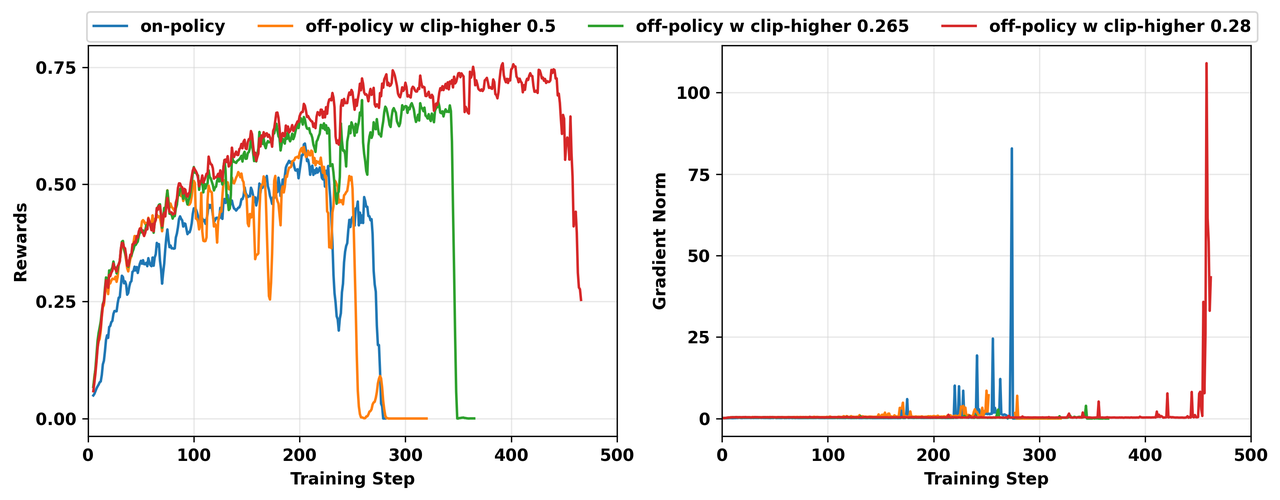
\includegraphics[width=\linewidth,height=0.64\textheight,keepaspectratio]{figures/image-01.png}
\caption*{\textbf{图 1。}Qwen3-14B-Base 上四次失败 GRPO TIR 实验的奖励（左）与梯度范数（右）。每个训练步均采样 1024 条轨迹（64 个提示 $\times$ 16 个响应），学习率为 $10^{-6}$。同策略与异策略实验的 \code{ppo_mini_batch_size} 分别为 1024 和 256。}
\end{figure}


% source-block: 291211a5-58b7-800e-b8b9-e7fec9a257a1 (callout; source-index: 7)

% source-block: 292211a5-58b7-80cb-b26d-f4398b15bb05 (text; source-index: 8)

\textbf{最新动态}（保留原文所列月日）


% source-block: 2bf211a5-58b7-80c8-a86a-d06945718bbc (text; source-index: 9)

\textbf{[12 月 2 日]} \href{https://arxiv.org/abs/2512.02556}{DeepSeek-V3.2} 采用了我们的\textbf{几何序列掩码}，用于处理训练与推理不匹配，以及一般异策略训练中的不稳定性。


% source-block: 2c3211a5-58b7-80da-a760-f6cdaa0f0c16 (text; source-index: 10)

\textbf{[12 月 1 日]} Qwen 团队在\href{https://arxiv.org/abs/2512.01374}{《稳定大语言模型强化学习：形式化与实践》}中讨论了我们的工作。


% source-block: 2a4211a5-58b7-80dd-85eb-facea672bd7c (text; source-index: 11)

\textbf{[11 月 12 日]} 面向一般异策略问题的 rollout 修正已合并至 VeRL：\href{https://verl.readthedocs.io/en/latest/algo/rollout_corr.html}{使用文档}、\href{https://verl.readthedocs.io/en/latest/algo/rollout_corr_math.html}{数学细节}。（\href{https://richardli.xyz/}{Yingru Li}）


% source-block: 2c1211a5-58b7-8048-9a1c-f48f0552fe53 (text; source-index: 12)

\textbf{[11 月 10 日]} 很高兴看到 \href{https://blog.vllm.ai/2025/11/10/bitwise-consistent-train-inference.html}{vLLM 博客}讨论了我们的工作，并实现了“逐比特一致的同策略强化学习”。


% source-block: 29d211a5-58b7-80a4-80bf-f01d038e7f08 (text; source-index: 13)

\textbf{[10 月 31 日]} VeRL 的全异步模块通过\href{https://github.com/volcengine/verl/pull/3955}{此 PR}集成了我们的工作。


% source-block: 29d211a5-58b7-8085-9333-d4ea9b6bca4f (text; source-index: 14)

\textbf{[10 月 20 日]} Slime 通过\href{https://github.com/THUDM/slime/pull/429}{此 PR}集成了我们的工作。（SGLang RL：\href{https://github.com/zhaochenyang20}{Chenyang Zhao}、\href{https://www.linkedin.com/in/jiajun-li-guapisolo/}{Jiajun Li}）


% source-block: 2c1211a5-58b7-807d-98df-e396b392553d (text; source-index: 15)

\textbf{[10 月 16 日]} 很高兴看到 Cognition 的 \href{https://cognition.ai/blog/swe-grep#motivation}{SWE-grep} 引用了我们的工作；它同样使用序列级掩码重要性采样（MIS）来处理训练与推理不匹配。


% source-block: 291211a5-58b7-80f1-9c73-f71a294cfc7d (text; source-index: 16)

\textbf{[10 月 15 日]} 一个 Megatron 训练崩溃问题通过几何级掩码得到解决。


% source-block: 291211a5-58b7-808d-870f-fcff431f4357 (external_object_instance; source-index: 17)

\href{https://github.com/volcengine/verl/issues/3597}{VeRL issue \#3597：使用 Qwen3-14B/Qwen3-30B-A3B 长时间运行 DAPO 时的 Megatron 训练崩溃。}


% source-block: 29d211a5-58b7-8053-bb32-c3122176e17b (text; source-index: 18)

\textbf{[10 月 13 日]} \href{https://github.com/volcengine/verl/releases/tag/v0.6.0}{VeRL 0.6.0} 已通过\href{https://github.com/volcengine/verl/pull/3694}{此 PR}集成我们的工作，包括新引入的\textbf{基于重要性权重几何平均值的序列掩码／拒绝方法（Geo-MIS/Geo-RS）}。（\href{https://richardli.xyz/}{Yingru Li}）


% source-block: 271211a5-58b7-80f7-8789-fd2833260f55 (callout; source-index: 19)

% source-block: 271211a5-58b7-808c-8d7b-caebe4c40799 (header; source-index: 20)

\hypertarget{src-271211a5-58b7-808c-8d7b-caebe4c40799}{}
\section*{内容提要}
\phantomsection
\addcontentsline{toc}{section}{内容提要}


% source-block: 277211a5-58b7-80a6-8d32-e5e211878239 (text; source-index: 21)

对推理速度的不懈追求，造成了危险的“训练与推理不匹配”，它可能悄无声息地破坏大语言模型强化学习。我们的研究揭示了一个恶性循环，在现代推理强化学习和智能体强化学习中尤为突出：


% source-block: 277211a5-58b7-804e-a899-cfa16040f0c7 (bulleted_list; source-index: 22)

\begin{itemize}

\item \textbf{分布外上下文促使模型采样低概率词元。}智能体工作流让模型接触外部输入和动态环境，使其频繁生成低概率词元；这些词元又是新颖推理、工具调用和适应性响应所必需的。（见\hyperlink{src-271211a5-58b7-8050-b3b1-dbbad2a1eb40}{第 3.4 节}。）

% source-block: 277211a5-58b7-80d9-ad38-ccdc1dfe9f5a (bulleted_list; source-index: 23)

\item \textbf{低概率词元加剧训练崩溃。}这些词元成为最薄弱的环节：训练与推理之间的不匹配在它们身上最为严重，会产生灾难性的大梯度，导致性能在无明显征兆的情况下下降，并突然训练失败。（见\hyperlink{src-271211a5-58b7-8043-9a6b-f4222291f060}{第 3.3 节}。）

% source-block: 277211a5-58b7-807d-900e-f24aa1b5c3f7 (bulleted_list; source-index: 24)

\item \textbf{硬件差异使问题更加复杂。}不同 GPU 架构可能以难以预测的方式加剧不匹配，因此同一套智能体训练配置可能在一台机器上成功，却在另一台机器上灾难性失败。（见\hyperlink{src-271211a5-58b7-80c9-ad90-f8aa1353bfe1}{第 3.5 节}。）

% source-block: 277211a5-58b7-8012-83a7-dd70b7fc9829 (bulleted_list; source-index: 25)

\item \textbf{序列级修正是有理论依据的解决方案。}序列级修正考虑完整的状态轨迹，修正有偏梯度，从而在不同硬件和复杂任务中恢复训练稳定性。（见\hyperlink{src-27b211a5-58b7-8099-ba48-fa8849ab54c8}{第 4.2.1 节}。）

\end{itemize}

% source-block: 2bd211a5-58b7-8033-a485-d9407b771feb (callout; source-index: 26)

% source-block: 2bd211a5-58b7-80b4-974c-c6987ef77b41 (header; source-index: 27)

\hypertarget{src-2bd211a5-58b7-80b4-974c-c6987ef77b41}{}
\section*{深入分析}
\phantomsection
\addcontentsline{toc}{section}{深入分析}


% source-block: 2bd211a5-58b7-808e-a28e-e287fc3822af (text; source-index: 28)

为更严格地剖析这一问题，我们还发表了由三篇博客构成的系列文章：


% source-block: 2c4211a5-58b7-802b-808c-f610d4db1d04 (bulleted_list; source-index: 29)

\begin{itemize}

\item \href{https://richardli.xyz/rl-collapse-1}{\textbf{第一篇：为什么异策略会破坏强化学习——SGA 分析框架。}}已有认识（TRPO 理论）：代理目标 $L_\mu(\pi)$ 是强化学习目标 $J(\pi)$ 的一阶泰勒近似；TRPO 下界 $J(\pi)\ge L_\mu(\pi)-C\cdot T^2\cdot D_{\mathrm{TV}}^{\max}$ 表明近似误差随 $T^2$ 增长，要求信赖域按 $\delta\propto 1/T^2$ 缩小。我们的见解是：词元级重要性采样（PPO/GRPO）计算的是 $\nabla L_\mu$，而非 $\nabla J$；它修正词元分布，却没有修正状态分布的不匹配（$d_\mu\ne d_\pi$），从而产生 $O(T^2D_{\mathrm{TV}}^{\max})$ 的偏差。我们通过 SGA 引理形式化了两种失效模式：由 $D_{\mathrm{TV}}$ 衡量的\textbf{偏差}，以及由 $\chi^2$ 散度衡量的\textbf{方差}；这两类指标不能互换。

% source-block: 2c4211a5-58b7-8030-bd63-d60722697c06 (bulleted_list; source-index: 30)

\item \href{https://richardli.xyz/rl-collapse-2}{\textbf{第二篇：应用 SGA 框架——词元级与序列级修正。}}我们的分析表明，词元级重要性采样（PPO/GRPO）因代理目标的一阶近似误差而具有 $O(T^2D_{\mathrm{TV}}^{\max})$ 的偏差；序列级重要性采样无偏，但具有指数级方差 $O((1+\bar{\chi}_{\max}^{\,2})^T)$。我们的方案是通过截断 $\rho(y)\to\min(\rho(y),C)$，使 Seq-TIS 获得可控的偏差与方差折中。核心结论是：这种偏差属于序列级问题，在不可忽略时需要序列级解决方案。

% source-block: 2c4211a5-58b7-8082-8edd-c06110f99479 (bulleted_list; source-index: 31)

\item \href{https://richardli.xyz/rl-collapse-3}{\textbf{第三篇：通过序列掩码实现信赖域优化。}}已有认识（TRPO 理论）：信赖域约束保证代理目标仍是有效近似。我们的方案包括：（1）Seq-MIS 通过拒绝机制 $\mathbb{I}(\rho\le C)\cdot\rho\cdot f$ 实施硬信赖域，完全排除分布外样本；（2）Geo-RS 使用几何平均值 $\rho_{\mathrm{geo}}=\rho^{1/T}$，实现与长度无关的逐词元信赖域。这是在大语言模型中实现 TRPO 硬信赖域的一种实用方式，可避免系统性地拒绝长序列。

\end{itemize}

% source-block: 2b8211a5-58b7-80c9-80fe-cd864e334308 (transclusion_container; source-index: 32)

% source-block: 271211a5-58b7-8057-a4a9-fe5550d04cb1 (header; source-index: 33)

\hypertarget{src-271211a5-58b7-8057-a4a9-fe5550d04cb1}{}
\section*{引用信息}
\phantomsection
\addcontentsline{toc}{section}{引用信息}


% source-block: 271211a5-58b7-80c0-bdba-f8043a361bcc (code; source-index: 34)

\lstinputlisting{source/original-citation.bib}

% Chinese translation assembled from source/blocks.json.

% See source/translation.py for the translation and source/build_tex.py for assembly.

% source-block: 271211a5-58b7-804d-b209-d12262749c7e (header; source-index: 35)

\hypertarget{src-271211a5-58b7-804d-b209-d12262749c7e}{}
\section*{1. 突然崩溃之谜}
\phantomsection
\addcontentsline{toc}{section}{1. 突然崩溃之谜}


% source-block: 277211a5-58b7-8038-b454-fcd3581d713a (text; source-index: 36)

大语言模型强化学习（LLM-RL）发展迅速，但一种令人困扰的突然训练崩溃现象正在出现。无论是复杂的推理强化学习，还是多轮智能体强化学习，许多人都观察到：训练在稳定学习一段时间后，会突然发生灾难性失败。


% source-block: 277211a5-58b7-802c-90e3-f0072fb4f4f6 (text; source-index: 37)

最近，我们在 Qwen3 模型上开展多轮工具集成推理（tool-integrated reasoning，TIR）的智能体强化学习实验时，亲身遇到了这个问题。在 L20 GPU 集群上，GRPO 算法的同策略和异策略变体均出现了这种情况。图 1 展示了四次 Qwen3-14B-Base 崩溃实验的奖励与梯度范数变化。随着训练进行，梯度范数突然爆炸，导致模型崩溃。我们最初排查了几个常见原因：


% source-block: 277211a5-58b7-8046-a918-f05a425996a9 (bulleted_list; source-index: 38)

\begin{itemize}

\item 检查代码，确认智能体循环遵循词元输入、词元输出（token-in-token-out）的过程。

% source-block: 277211a5-58b7-8058-b17d-ffc5b440e8cb (bulleted_list; source-index: 39)

\item 调整 Adam 优化器的超参数 \code{beta1} 和 \code{beta2}。

% source-block: 277211a5-58b7-8002-b0e4-cb7b0d947723 (bulleted_list; source-index: 40)

\item 对优势值进行批量归一化，以平衡更新。

% source-block: 277211a5-58b7-8066-a42e-ebf293d000c7 (text; source-index: 41)

\ldots


\end{itemize}

% source-block: 277211a5-58b7-8093-83f9-e7226af53cb1 (text; source-index: 42)

然而，这些常规修复均未奏效。由于连更简单的同策略实验也会失败，我们怀疑问题来自训练栈中更基础的部分。这促使我们研究现代 LLM-RL 中一个关键且日益普遍的挑战：高度优化的推理引擎与忠实执行训练计算的框架之间，存在不可避免的差距。


% source-block: 277211a5-58b7-806b-ad86-d2218563a53a (divider; source-index: 43)

% Chinese translation assembled from source/blocks.json.

% See source/translation.py for the translation and source/build_tex.py for assembly.

% source-block: 271211a5-58b7-8068-bb2e-fda81fd79c4b (header; source-index: 44)

\hypertarget{src-271211a5-58b7-8068-bb2e-fda81fd79c4b}{}
\section*{2. 根本冲突：推理与训练之间不断扩大的差距}
\phantomsection
\addcontentsline{toc}{section}{2. 根本冲突：推理与训练之间不断扩大的差距}


% source-block: 271211a5-58b7-8075-ad1d-e1c28508a69d (text; source-index: 45)

轨迹生成（rollout）的速度是 LLM-RL 的核心瓶颈。为满足巨大的吞吐量需求，现代推理引擎（如 vLLM、SGLang、TensorRT-LLM）采用了激进的优化策略，包括推测解码、低精度计算（INT8/FP8），以及针对特定批量设置优化、计算随批量变化的 CUDA 内核。在维持采样保真度的同时，现代推理引擎的首要目标是最大化吞吐量，通常以每秒词元数衡量。

训练框架（如 FSDP、DeepSpeed、Megatron-LM）则需要采取不同的权衡，优先保证梯度计算的数值稳定性与精度，往往为主权重和优化器状态使用 FP32 等更高精度格式。优化优先级与约束条件的不同，造成了不可避免的训练与推理不匹配。对更快 rollout 的持续追求正在扩大这一差距。

有人可能会建议强制两端采用相同计算，例如使用\href{https://thinkingmachines.ai/blog/defeating-nondeterminism-in-llm-inference/}{“批量无关内核”}，但这些方案会带来严重的性能损失，削弱使用高速推理引擎的意义。速度与一致性之间的权衡，正是问题的核心，使其成为一个持续存在的挑战。


% source-block: 271211a5-58b7-80ca-a1d1-d18bc503801a (text; source-index: 46)

在我们的技术栈中，这种不匹配出现在 vLLM 推理采样器与 FSDP 训练器之间。实际执行的参数更新为：


% source-block: 271211a5-58b7-805a-8edc-d856427744e3 (equation; source-index: 47)


\[
\adjustbox{max width=0.98\linewidth}{$\displaystyle \mathbb{E} _{x\sim \mathcal{D}}\mathbb{E} _{y\sim \textcolor{red}{\pi _{\theta}^{\mathrm{vllm}}}\left( \cdot |x \right)}\left[ R\left( x,y \right) \nabla _{\theta}\log \textcolor{blue}{\pi _{\theta}^{\mathrm{fsdp}}}\left( y|x \right) \right],$}
\]


% source-block: 271211a5-58b7-8075-8d39-edad869719ad (text; source-index: 48)

而理论上应当使用的参数更新为：


% source-block: 271211a5-58b7-8096-bc46-dbecb4d4e6e5 (equation; source-index: 49)


\[
\adjustbox{max width=0.98\linewidth}{$\displaystyle \mathbb{E} _{x\sim \mathcal{D}}\mathbb{E} _{y\sim \textcolor{blue}{\pi _{\theta}^{\mathrm{fsdp}}}\left( \cdot |x \right)}\left[ R\left( x,y \right) \nabla _{\theta}\log \textcolor{blue}{\pi _{\theta}^{\mathrm{fsdp}}}\left( y|x \right) \right].$}
\]


% source-block: 271211a5-58b7-8022-ab19-dc1c49af2929 (text; source-index: 50)

其中，$x$ 是从分布 $\mathcal D$ 中采样的提示，$y$ 是响应，$R$ 是奖励函数，$\theta$ 是大语言模型参数，$\piv$ 与 $\pif$ 分别是由 vLLM 引擎和 FSDP 引擎实现的策略。要研究这一问题，我们首先需要一种度量方法。


% source-block: 277211a5-58b7-80bb-8063-e98e153b97c9 (divider; source-index: 51)

% Chinese translation assembled from source/blocks.json.

% See source/translation.py for the translation and source/build_tex.py for assembly.

% source-block: 271211a5-58b7-8046-af48-c3129693f3f1 (header; source-index: 52)

\hypertarget{src-271211a5-58b7-8046-af48-c3129693f3f1}{}
\section*{3. 剖析训练崩溃}
\phantomsection
\addcontentsline{toc}{section}{3. 剖析训练崩溃}


% source-block: 271211a5-58b7-80f8-b824-f71b5fe11763 (sub_header; source-index: 53)

\hypertarget{src-271211a5-58b7-80f8-b824-f71b5fe11763}{}
\subsection*{3.0 实验设置}
\phantomsection
\addcontentsline{toc}{subsection}{3.0 实验设置}


% source-block: 271211a5-58b7-8011-872c-ff8c4e24455f (text; source-index: 54)

除非另有说明，第 3 节和第 4 节的实验均在 \href{https://github.com/search?q=verl&type=repositories}{VeRL} 框架下采用 TIR 设置进行，使用 vLLM v1 采样器（AsyncvLLMServer）、Qwen3-14B-Base 模型和 GRPO 算法，并在 L20 GPU 集群上运行。


% source-block: 277211a5-58b7-80de-809d-ed58cc96a034 (divider; source-index: 55)

% source-block: 271211a5-58b7-8057-8bd8-da62a18d6e3a (sub_header; source-index: 56)

\hypertarget{src-271211a5-58b7-8057-8bd8-da62a18d6e3a}{}
\subsection*{3.1 度量不匹配：\texttt{vllm-kl} 指标}
\phantomsection
\addcontentsline{toc}{subsection}{3.1 度量不匹配：vllm-kl 指标}


% source-block: 271211a5-58b7-80be-bf0e-d70767335f76 (text; source-index: 57)

一种直接衡量训练与推理不匹配的指标是 \code{vllm-kl}：


% source-block: 271211a5-58b7-80f6-9ba6-e24d819d0485 (equation; source-index: 58)


\[
\adjustbox{max width=0.98\linewidth}{$\displaystyle \mathbb{E}_{s\sim d_{\textcolor{red}{\pi^{\text{vllm}}_\theta}}}\left[\text{KL}\left(\textcolor{red}{\pi^{\text{vllm}}_\theta}\left(\cdot|s\right),\textcolor{blue}{\pi^{\text{fsdp}}_\theta}\left(\cdot|s\right)\right)\right]$}
\]

\vspace{-1em}

\[
\adjustbox{max width=0.98\linewidth}{$\displaystyle {}= \mathbb{E}_{s\sim d_{\textcolor{red}{\pi^{\text{vllm}}_\theta}},a\sim {\textcolor{red}{\pi^{\text{vllm}}_\theta}\left(\cdot|s\right)}} \left[\log\left(\frac{\textcolor{red}{\pi^{\text{vllm}}_\theta}(a|s)}{\textcolor{blue}{\pi^{\text{fsdp}}_\theta}(a|s)}\right)\right],$}
\]


% source-block: 271211a5-58b7-80c4-a955-ea90e314216d (text; source-index: 59)

其中，$d_\pi$ 是策略 $\pi$ 的状态占用测度，$s$ 是上下文前缀（状态），$a$ 是词元（动作）。我们的实验涉及工具调用，因此响应 $y$ 可能包含工具返回内容；\code{vllm-kl} 指标只统计模型自身生成的词元。假设已能取得推理引擎的词元概率，下面的代码给出了在 \href{https://github.com/search?q=verl&type=repositories}{VeRL} 中使用 \href{http://joschu.net/blog/kl-approx.html}{K3 估计器}计算该指标的实现。


% source-block: 271211a5-58b7-804d-a515-cf72e195691b (toggle; source-index: 60)

\hypertarget{src-271211a5-58b7-804d-a515-cf72e195691b}{}
\paragraph*{\texttt{vllm-kl} 的 K3 估计器代码（展开原文折叠内容）}


% source-block: 271211a5-58b7-8012-a9f1-e15e76434fd9 (code; source-index: 61)

\lstinputlisting{source/k3_vllm_kl.py}

% source-block: 277211a5-58b7-80e1-92cf-f20011be2769 (divider; source-index: 62)

% source-block: 271211a5-58b7-806f-a251-c6e6bcade90c (sub_header; source-index: 63)

\hypertarget{src-271211a5-58b7-806f-a251-c6e6bcade90c}{}
\subsection*{3.2 预警信号：相互关联的不稳定性}
\phantomsection
\addcontentsline{toc}{subsection}{3.2 预警信号：相互关联的不稳定性}


% source-block: 271211a5-58b7-8043-b721-efdbf1c851cb (text; source-index: 64)

第一个线索是：高 \code{vllm-kl} 值并非孤立事件，而是与其他不稳定迹象高度相关。


% source-block: 271211a5-58b7-80e6-a27d-df95d40e31e0 (sub_sub_header; source-index: 65)

\hypertarget{src-271211a5-58b7-80e6-a27d-df95d40e31e0}{}
\subsubsection*{3.2.1 FSDP 熵与奖励的波动}


% source-block: 271211a5-58b7-808f-a90f-df4730390799 (text; source-index: 66)

在许多实验中，我们观察到 \code{vllm-kl} 的异常尖峰通常会同时伴随 FSDP 策略 $\pif$ 的熵与奖励的异常波动。图 2 给出了直观例子：熵尖峰与 \code{vllm-kl} 尖峰的位置几乎完全对应。奖励没有表现出同样明显的相关性，但在约第 250 步处，巨大的 \code{vllm-kl} 尖峰触发了一个低质量批次的生成，奖励也随之明显下跌。这意味着当不匹配较大时，vLLM 策略 $\piv$ 与 FSDP 策略 $\pif$ 都进入了不稳定区域。


% source-block: 271211a5-58b7-8055-8f35-c4a618ee5fed (image; source-index: 67)

\begin{figure}[H]
\centering
% source-block: 271211a5-58b7-8055-8f35-c4a618ee5fed (image)
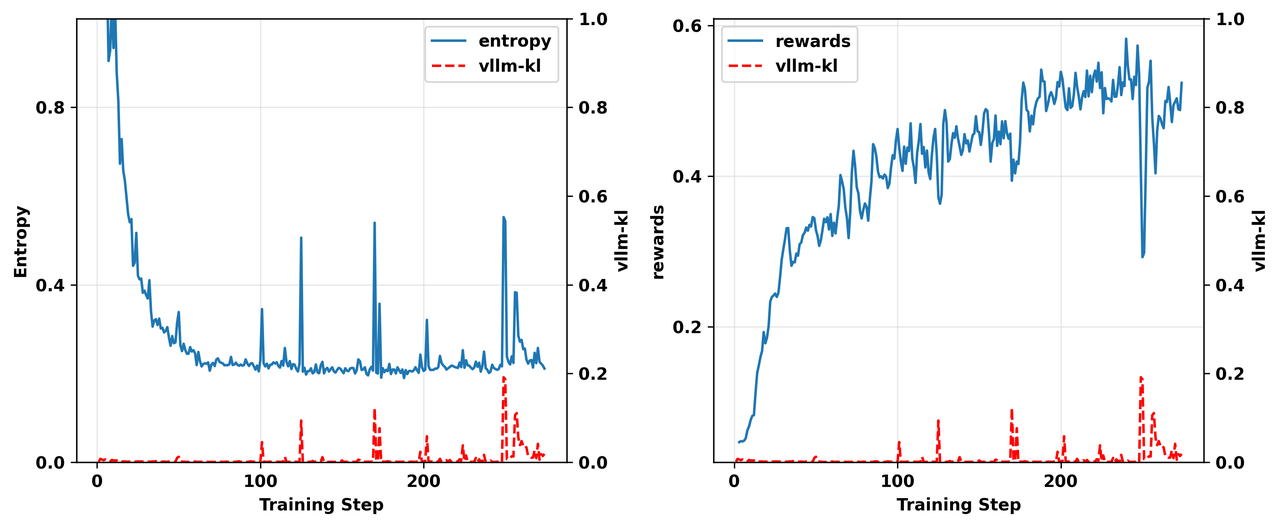
\includegraphics[width=\linewidth,height=0.64\textheight,keepaspectratio]{figures/image-02.png}
\caption*{\textbf{图 2。}同策略实验的熵（左）、奖励（右）与 \code{vllm-kl} 的对照，展示训练期间它们之间的相关性。}
\end{figure}


% source-block: 277211a5-58b7-805f-b028-ed2aaa0553fc (divider; source-index: 68)

% source-block: 271211a5-58b7-80b3-b8f8-eb93ea995636 (sub_sub_header; source-index: 69)

\hypertarget{src-271211a5-58b7-80b3-b8f8-eb93ea995636}{}
\subsubsection*{3.2.2 FSDP 困惑度和梯度范数上升，最终导致策略崩溃}


% source-block: 271211a5-58b7-8048-9746-ef5351a74003 (text; source-index: 70)

更关键的是，我们观察到 \code{vllm-kl} 的尖峰会同时伴随 \code{fsdp-ppl} 指标和梯度范数的爆炸。在实验中，响应 $y$ 的 FSDP \href{https://www.wikiwand.com/en/articles/Perplexity}{困惑度（PPL）}计算如下：


% source-block: 271211a5-58b7-8054-8737-dd5a1b74c83c (equation; source-index: 71)


\[
\adjustbox{max width=0.98\linewidth}{$\displaystyle \text{fsdp-ppl}:  \exp\left(\frac{-1}{\left| \mathcal{T} _{\mathcal{M}}\left( y \right) \right|}\sum_{t\in \mathcal{T} _{\mathcal{M}}\left( y \right)}{\log \textcolor{blue}{\pi _{\theta}^{\text{fsdp}}}\left( y_t|y_{<t} \right)}\right)$}
\]


% source-block: 271211a5-58b7-80a7-bc39-d63c27611086 (text; source-index: 72)

其中，$\mathcal T_{\mathcal M}(y)$ 是响应 $y$ 中由模型自身生成的词元索引集合。最终的 \code{fsdp-ppl} 指标，是一个批次中所有响应的困惑度的平均值。图 3 展示了同策略与异策略两种 GRPO 实验结果。两次实验中，\code{vllm-kl} 的尖峰几乎都精确对应着 \code{fsdp-ppl} 和梯度范数的爆炸。此外，训练奖励崩溃之前，\code{vllm-kl} 已经明显上升。


% source-block: 271211a5-58b7-8012-87d3-ce3f15ed3061 (image; source-index: 73)

\begin{figure}[H]
\centering
% source-block: 271211a5-58b7-8012-87d3-ce3f15ed3061 (image)
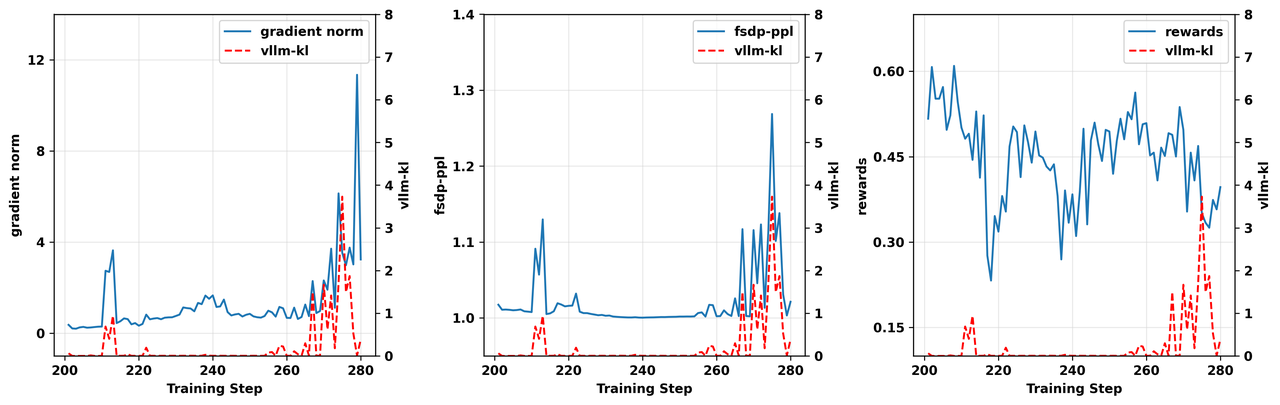
\includegraphics[width=\linewidth,height=0.64\textheight,keepaspectratio]{figures/image-03.png}
\par\smallskip
% source-block: 271211a5-58b7-8046-aba6-f54c74a49cf2 (image)
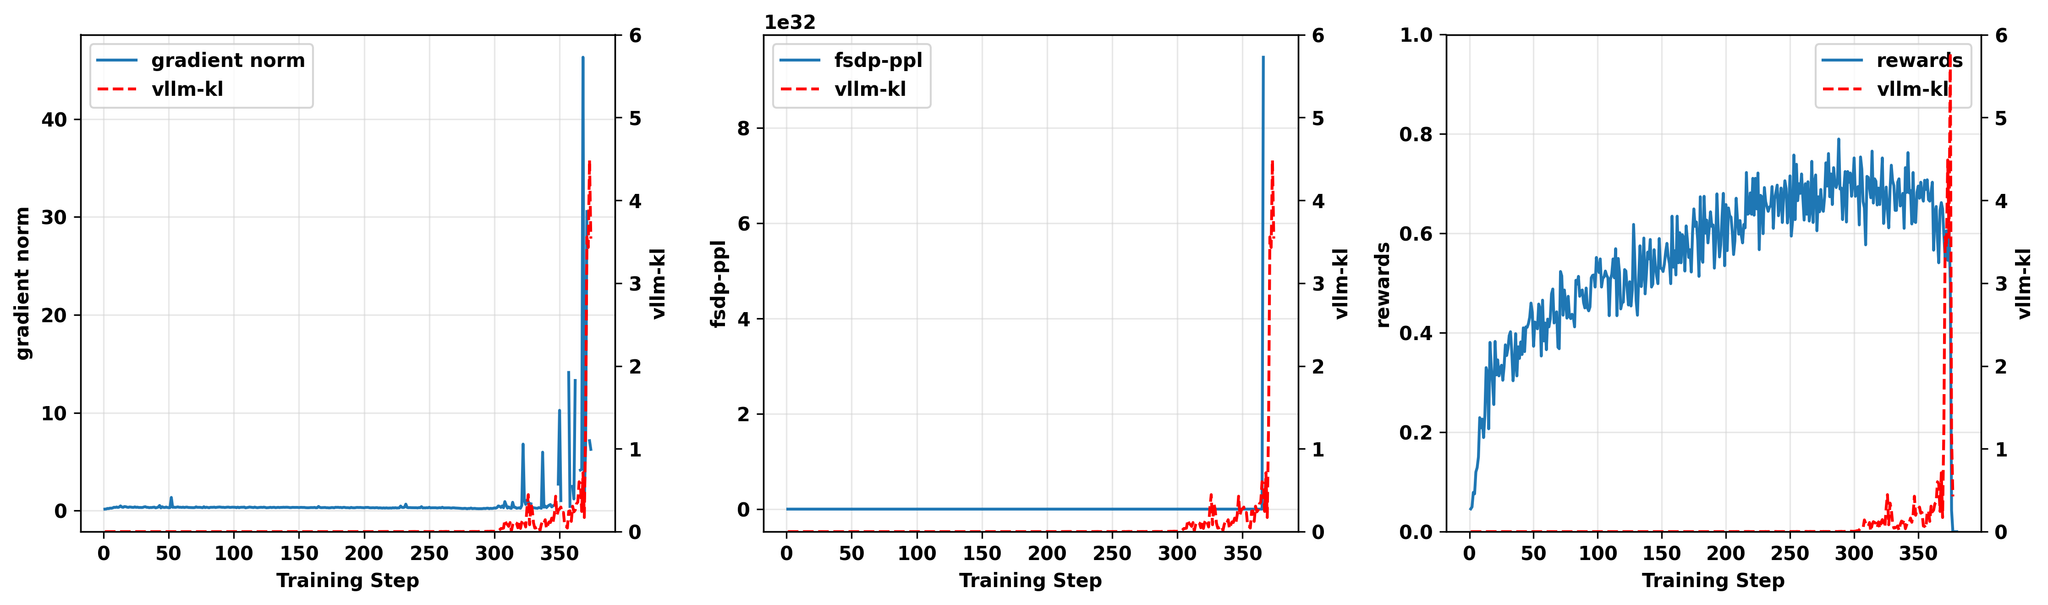
\includegraphics[width=\linewidth,height=0.64\textheight,keepaspectratio]{figures/image-04.png}
\par\smallskip
\caption*{\textbf{图 3。}同策略实验第 200--280 步的结果（上），以及 \code{clip-higher=0.28} 的异策略实验结果（下）。梯度范数（左）、\code{fsdp-ppl}（中）、奖励（右）分别与 \code{vllm-kl} 对照，展示训练期间的相关性。}
\end{figure}


% source-block: 271211a5-58b7-8046-aba6-f54c74a49cf2 (image; source-index: 74)

% source-block: 271211a5-58b7-80f1-b8fd-fd93435d5365 (text; source-index: 75)

在我们的实验中，模型自身生成的序列至少包含几百个词元，因此作者认为，在训练后期 PPL 维持在 1 附近更为合理。然而，在训练与推理不匹配显著、即 \code{vllm-kl} 很高的批次中，\code{fsdp-ppl} 出现了爆炸。这表明，FSDP 引擎为推理策略采样得到的词元分配了灾难性低的概率，从而导致梯度爆炸。这一观察帮助我们进一步定位不匹配更容易发生的位置。后文将看到：这些 FSDP 概率极低的词元在被采样时，其 vLLM 概率远没有这么低。


% source-block: 277211a5-58b7-8053-933b-eb574993d0ce (divider; source-index: 76)

% source-block: 271211a5-58b7-8043-9a6b-f4222291f060 (sub_header; source-index: 77)

\hypertarget{src-271211a5-58b7-8043-9a6b-f4222291f060}{}
\subsection*{3.3 关键证据：低概率词元陷阱}
\phantomsection
\addcontentsline{toc}{subsection}{3.3 关键证据：低概率词元陷阱}


% source-block: 277211a5-58b7-8056-afbf-fa0d227e8459 (text; source-index: 78)

\textbf{不匹配并非均匀发生。}


% source-block: 277211a5-58b7-804c-b071-d15a4d40365e (text; source-index: 79)

通过分析 \code{vllm-kl} 水平不同的批次，我们发现了鲜明的模式：\textbf{对 vLLM 推理引擎而言概率较低的词元，其偏差最为严重。}当词元的推理概率趋近于零时，训练概率可能进一步低上多个数量级，导致 PPL 和梯度趋于无穷。为尽量提高结论的普适性，我们从不同实验、不同训练步中，选取了崩溃之前采样的批次。这些批次均具有相对较高的 \code{vllm-kl}，便于在现象明显的条件下研究不匹配模式。我们按以下三个区间收集 rollout 批次，每组包含五个批次，约 500 万个词元：


% source-block: 271211a5-58b7-8010-8a35-e7633703fd9b (bulleted_list; source-index: 80)

\begin{itemize}

\item \textbf{第 1 组（低）：}每个 rollout 批次的 \code{vllm-kl} 不大于 $10^{-3}$，使用 H20 GPU 采样。

% source-block: 271211a5-58b7-8015-93c9-e4e2ef8301f1 (bulleted_list; source-index: 81)

\item \textbf{第 2 组（中）：}每个 rollout 批次的 \code{vllm-kl} 位于 $[10^{-3},2\times10^{-2}]$，使用 L20 GPU 采样。

% source-block: 271211a5-58b7-800a-88cd-e2fe0fb1c394 (bulleted_list; source-index: 82)

\item \textbf{第 3 组（高）：}每个 rollout 批次的 \code{vllm-kl} 位于 $[2\times10^{-2},10^{-1}]$，使用 L20 GPU 采样。

\end{itemize}

% source-block: 271211a5-58b7-80dd-83a4-c319ae9b7b6d (text; source-index: 83)

图 4(a)、4(b)、4(c) 展示了不同 \code{vllm-kl} 量级下，vLLM 输出概率 $\piv(a\mid s)$ 与不匹配程度 $\log\pif(a\mid s)-\log\piv(a\mid s)$ 之间的关系。


% source-block: 271211a5-58b7-8025-976d-c69c3de0ef2d (image; source-index: 84)

\begin{figure}[H]
\centering
% source-block: 271211a5-58b7-8025-976d-c69c3de0ef2d (image)
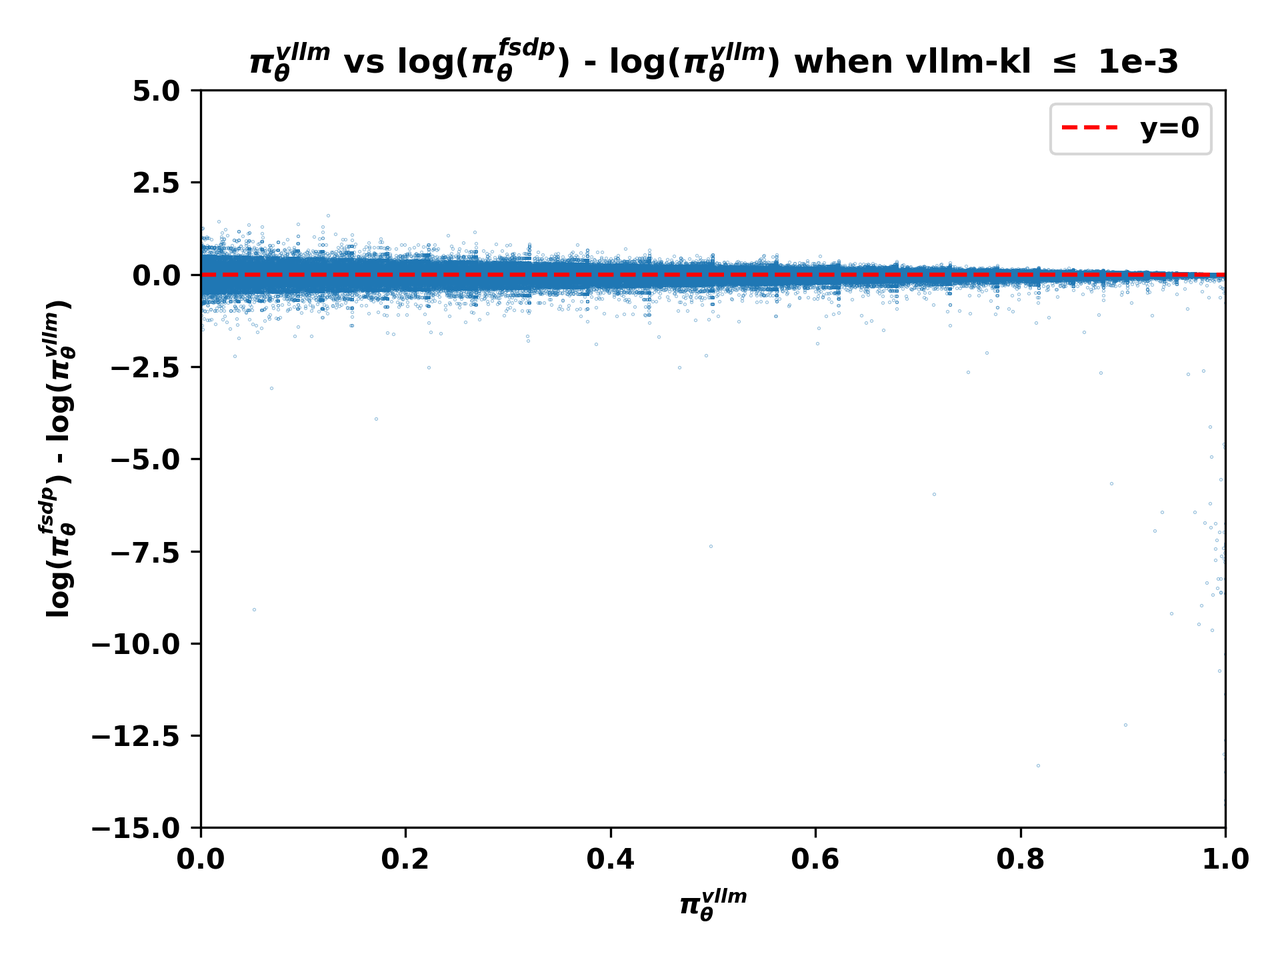
\includegraphics[width=\linewidth,height=0.64\textheight,keepaspectratio]{figures/image-05.png}
\caption*{\textbf{图 4(a)。}第 1 组批次中，词元的 $\piv$ 与 $\log\pif-\log\piv$ 的关系。}
\end{figure}


% source-block: 271211a5-58b7-8084-87e0-d30121785272 (image; source-index: 85)

\begin{figure}[H]
\centering
% source-block: 271211a5-58b7-8084-87e0-d30121785272 (image)
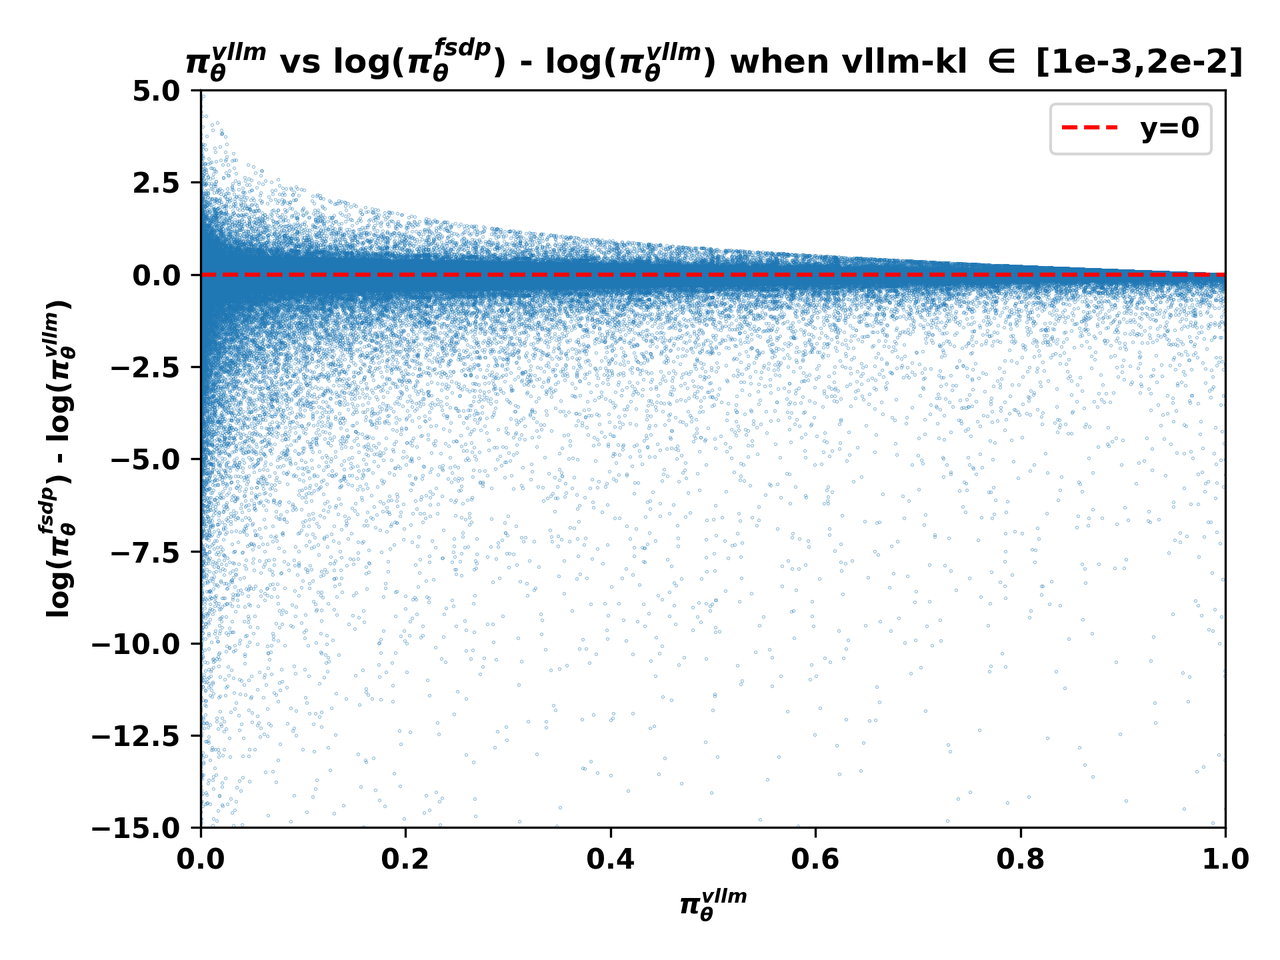
\includegraphics[width=\linewidth,height=0.64\textheight,keepaspectratio]{figures/image-06.png}
\caption*{\textbf{图 4(b)。}第 2 组批次中，词元的 $\piv$ 与 $\log\pif-\log\piv$ 的关系。}
\end{figure}


% source-block: 271211a5-58b7-8092-a67e-f3089c4cf067 (image; source-index: 86)

\begin{figure}[H]
\centering
% source-block: 271211a5-58b7-8092-a67e-f3089c4cf067 (image)
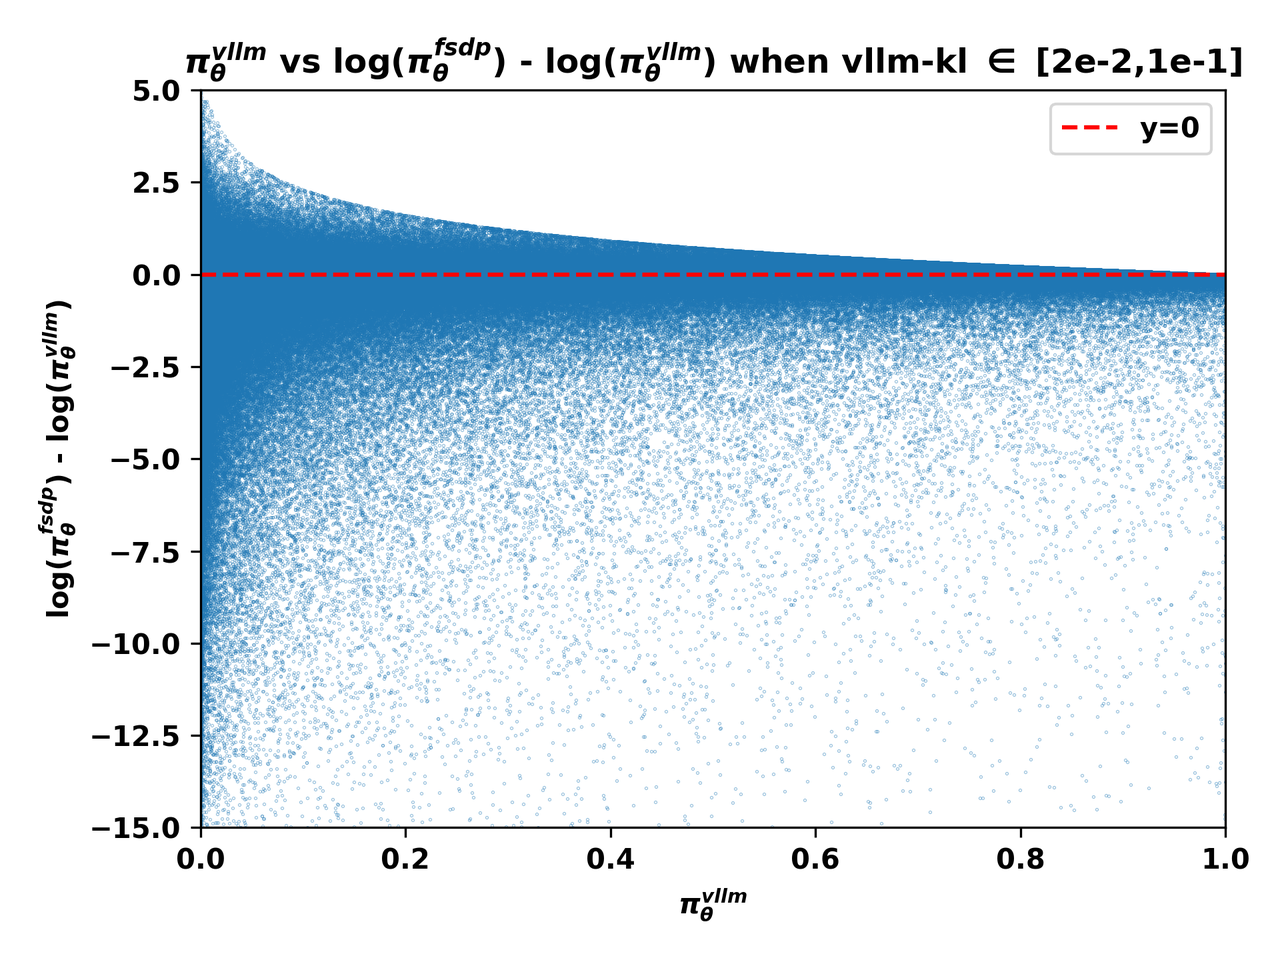
\includegraphics[width=\linewidth,height=0.64\textheight,keepaspectratio]{figures/image-07.png}
\caption*{\textbf{图 4(c)。}第 3 组批次中，词元的 $\piv$ 与 $\log\pif-\log\piv$ 的关系。}
\end{figure}


% source-block: 271211a5-58b7-805f-bcbf-d246ba54362d (text; source-index: 87)

从以上三幅图中，可以清楚观察到：


% source-block: 271211a5-58b7-800a-88b0-cb2ff65c7b6d (numbered_list; source-index: 88)

\begin{enumerate}

\item 当 vLLM 概率 $\piv$ 趋近于零时，不匹配通常更加明显，$\log\pif-\log\piv$ 也更容易出现极端值。

% source-block: 271211a5-58b7-80a8-8b79-d87b04cf6f3c (numbered_list; source-index: 89)

\item L20 GPU 上收集的批次，即第 2、3 组，其训练与推理不匹配主要表现为 FSDP 概率 $\pif$ 显著小于 vLLM 概率 $\piv$。

\end{enumerate}

% source-block: 277211a5-58b7-80bc-ae1a-df54182c0628 (divider; source-index: 90)

% source-block: 271211a5-58b7-8050-b3b1-dbbad2a1eb40 (sub_header; source-index: 91)

\hypertarget{src-271211a5-58b7-8050-b3b1-dbbad2a1eb40}{}
\subsection*{3.4 分布外工具响应放大不匹配}
\phantomsection
\addcontentsline{toc}{subsection}{3.4 分布外工具响应放大不匹配}


% source-block: 277211a5-58b7-80d0-9d87-e202276dc7f9 (sub_sub_header; source-index: 92)

\hypertarget{src-277211a5-58b7-80d0-9d87-e202276dc7f9}{}
\subsubsection*{3.4.1 非首轮输出中的不匹配更严重}


% source-block: 271211a5-58b7-8079-8ad0-d72e0e85ce0b (text; source-index: 93)

第 3 节的发现解释了为什么多轮 TIR 实验中的问题如此突出，尤其是在模型的非首轮输出中。具体过程如下：


% source-block: 271211a5-58b7-809e-8568-f3c1bf646337 (numbered_list; source-index: 94)

\begin{enumerate}

\item 智能体收到工具响应，通常是结构化文本，例如由 \code{<python_output>} 和 \code{</python_output>} 标签包裹的上下文。与预训练和 SFT 数据相比，这类文本属于分布外（OOD）输入。

% source-block: 271211a5-58b7-80a2-82b3-da8b60bb1fdf (numbered_list; source-index: 95)

\item 面对不熟悉的分布外上下文，智能体策略的不确定性增加，因此在后续轮次中更容易采样低概率词元；\href{https://github.com/ltzheng/SimpleTIR}{SimpleTIR} 也观察到了这一现象。

% source-block: 271211a5-58b7-80e1-905f-e8e323252c50 (numbered_list; source-index: 96)

\item 如前所述，低概率词元正是严重不匹配的主要发生位置，因此会为 \code{fsdp-ppl} 和梯度爆炸创造条件。

\end{enumerate}

% source-block: 271211a5-58b7-807f-8974-ccd834bcb702 (text; source-index: 97)

接下来，我们可视化了三组批次中的不匹配情况，每组约 5000 条轨迹，重点比较模型首轮输出与非首轮输出的差异。我们使用两种可视化方式：


% source-block: 271211a5-58b7-8090-a724-cd2cf4996307 (numbered_list; source-index: 98)

\begin{enumerate}

\item \textbf{对数困惑度散点图：}横轴为 vLLM 策略 $\piv$ 计算的困惑度的对数，记作 \code{vllm-log-ppl}；纵轴为 FSDP 策略 $\pif$ 计算的困惑度的对数，记作 \code{fsdp-log-ppl}。

% source-block: 271211a5-58b7-80f8-a083-d8dd1fc23b4c (numbered_list; source-index: 99)

\item \textbf{概率散点图：}横轴为 vLLM 策略 $\piv$ 的词元概率，纵轴为 FSDP 策略 $\pif$ 的词元概率。

\end{enumerate}

% source-block: 271211a5-58b7-80da-a68a-cf9a7e67be87 (text; source-index: 100)

下面给出三组不匹配情况的可视化结果。


% source-block: 271211a5-58b7-802e-8f1c-fa8e9902f933 (bulleted_list; source-index: 101)

\begin{itemize}

\item \textbf{第 1 组：}\code{vllm-kl} $\le10^{-3}$ 的批次。

\end{itemize}

% source-block: 271211a5-58b7-805e-af00-de25affd1d4a (image; source-index: 102)

\begin{figure}[H]
\centering
% source-block: 271211a5-58b7-805e-af00-de25affd1d4a (image)
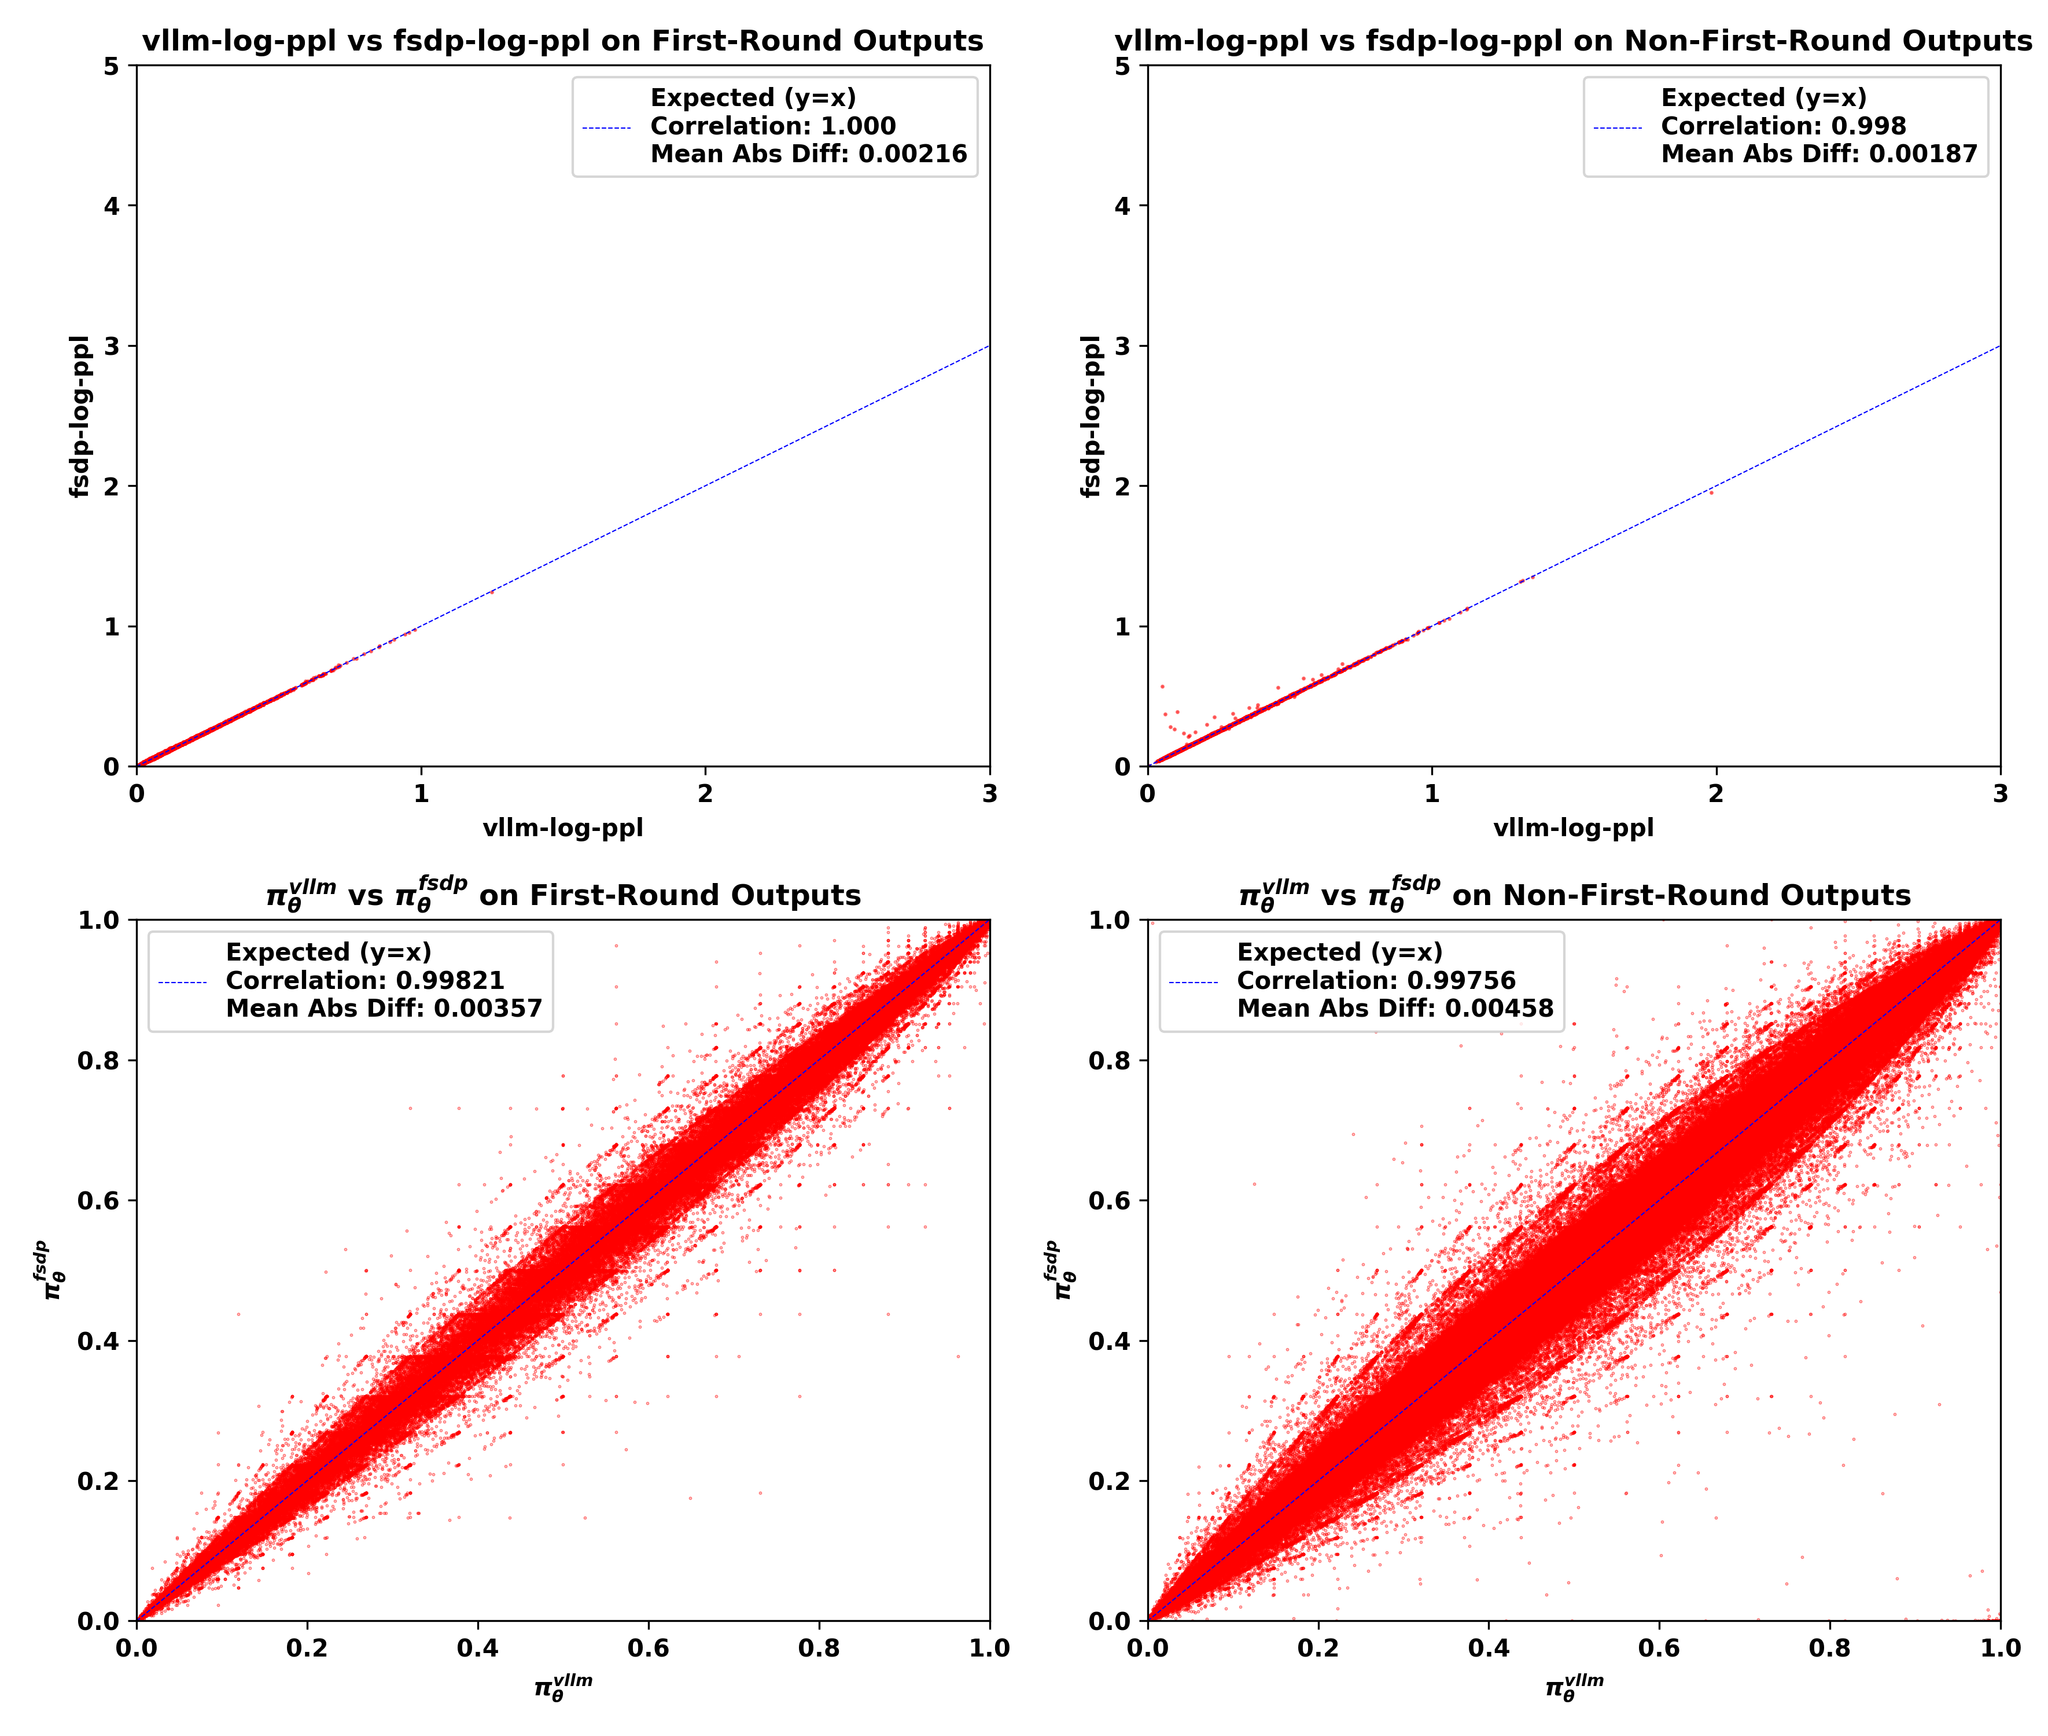
\includegraphics[width=\linewidth,height=0.64\textheight,keepaspectratio]{figures/image-08.png}
\caption*{第 1 组首轮与非首轮输出的不匹配可视化（原文未编号）：\code{vllm-kl} $\le10^{-3}$。}
\end{figure}


% source-block: 271211a5-58b7-804e-84f9-ca41fc298777 (bulleted_list; source-index: 103)

\begin{itemize}

\item \textbf{第 2 组：}\code{vllm-kl} $\in[10^{-3},2\times10^{-2}]$ 的批次。

\end{itemize}

% source-block: 271211a5-58b7-80cb-8597-da22a85d90da (image; source-index: 104)

\begin{figure}[H]
\centering
% source-block: 271211a5-58b7-80cb-8597-da22a85d90da (image)
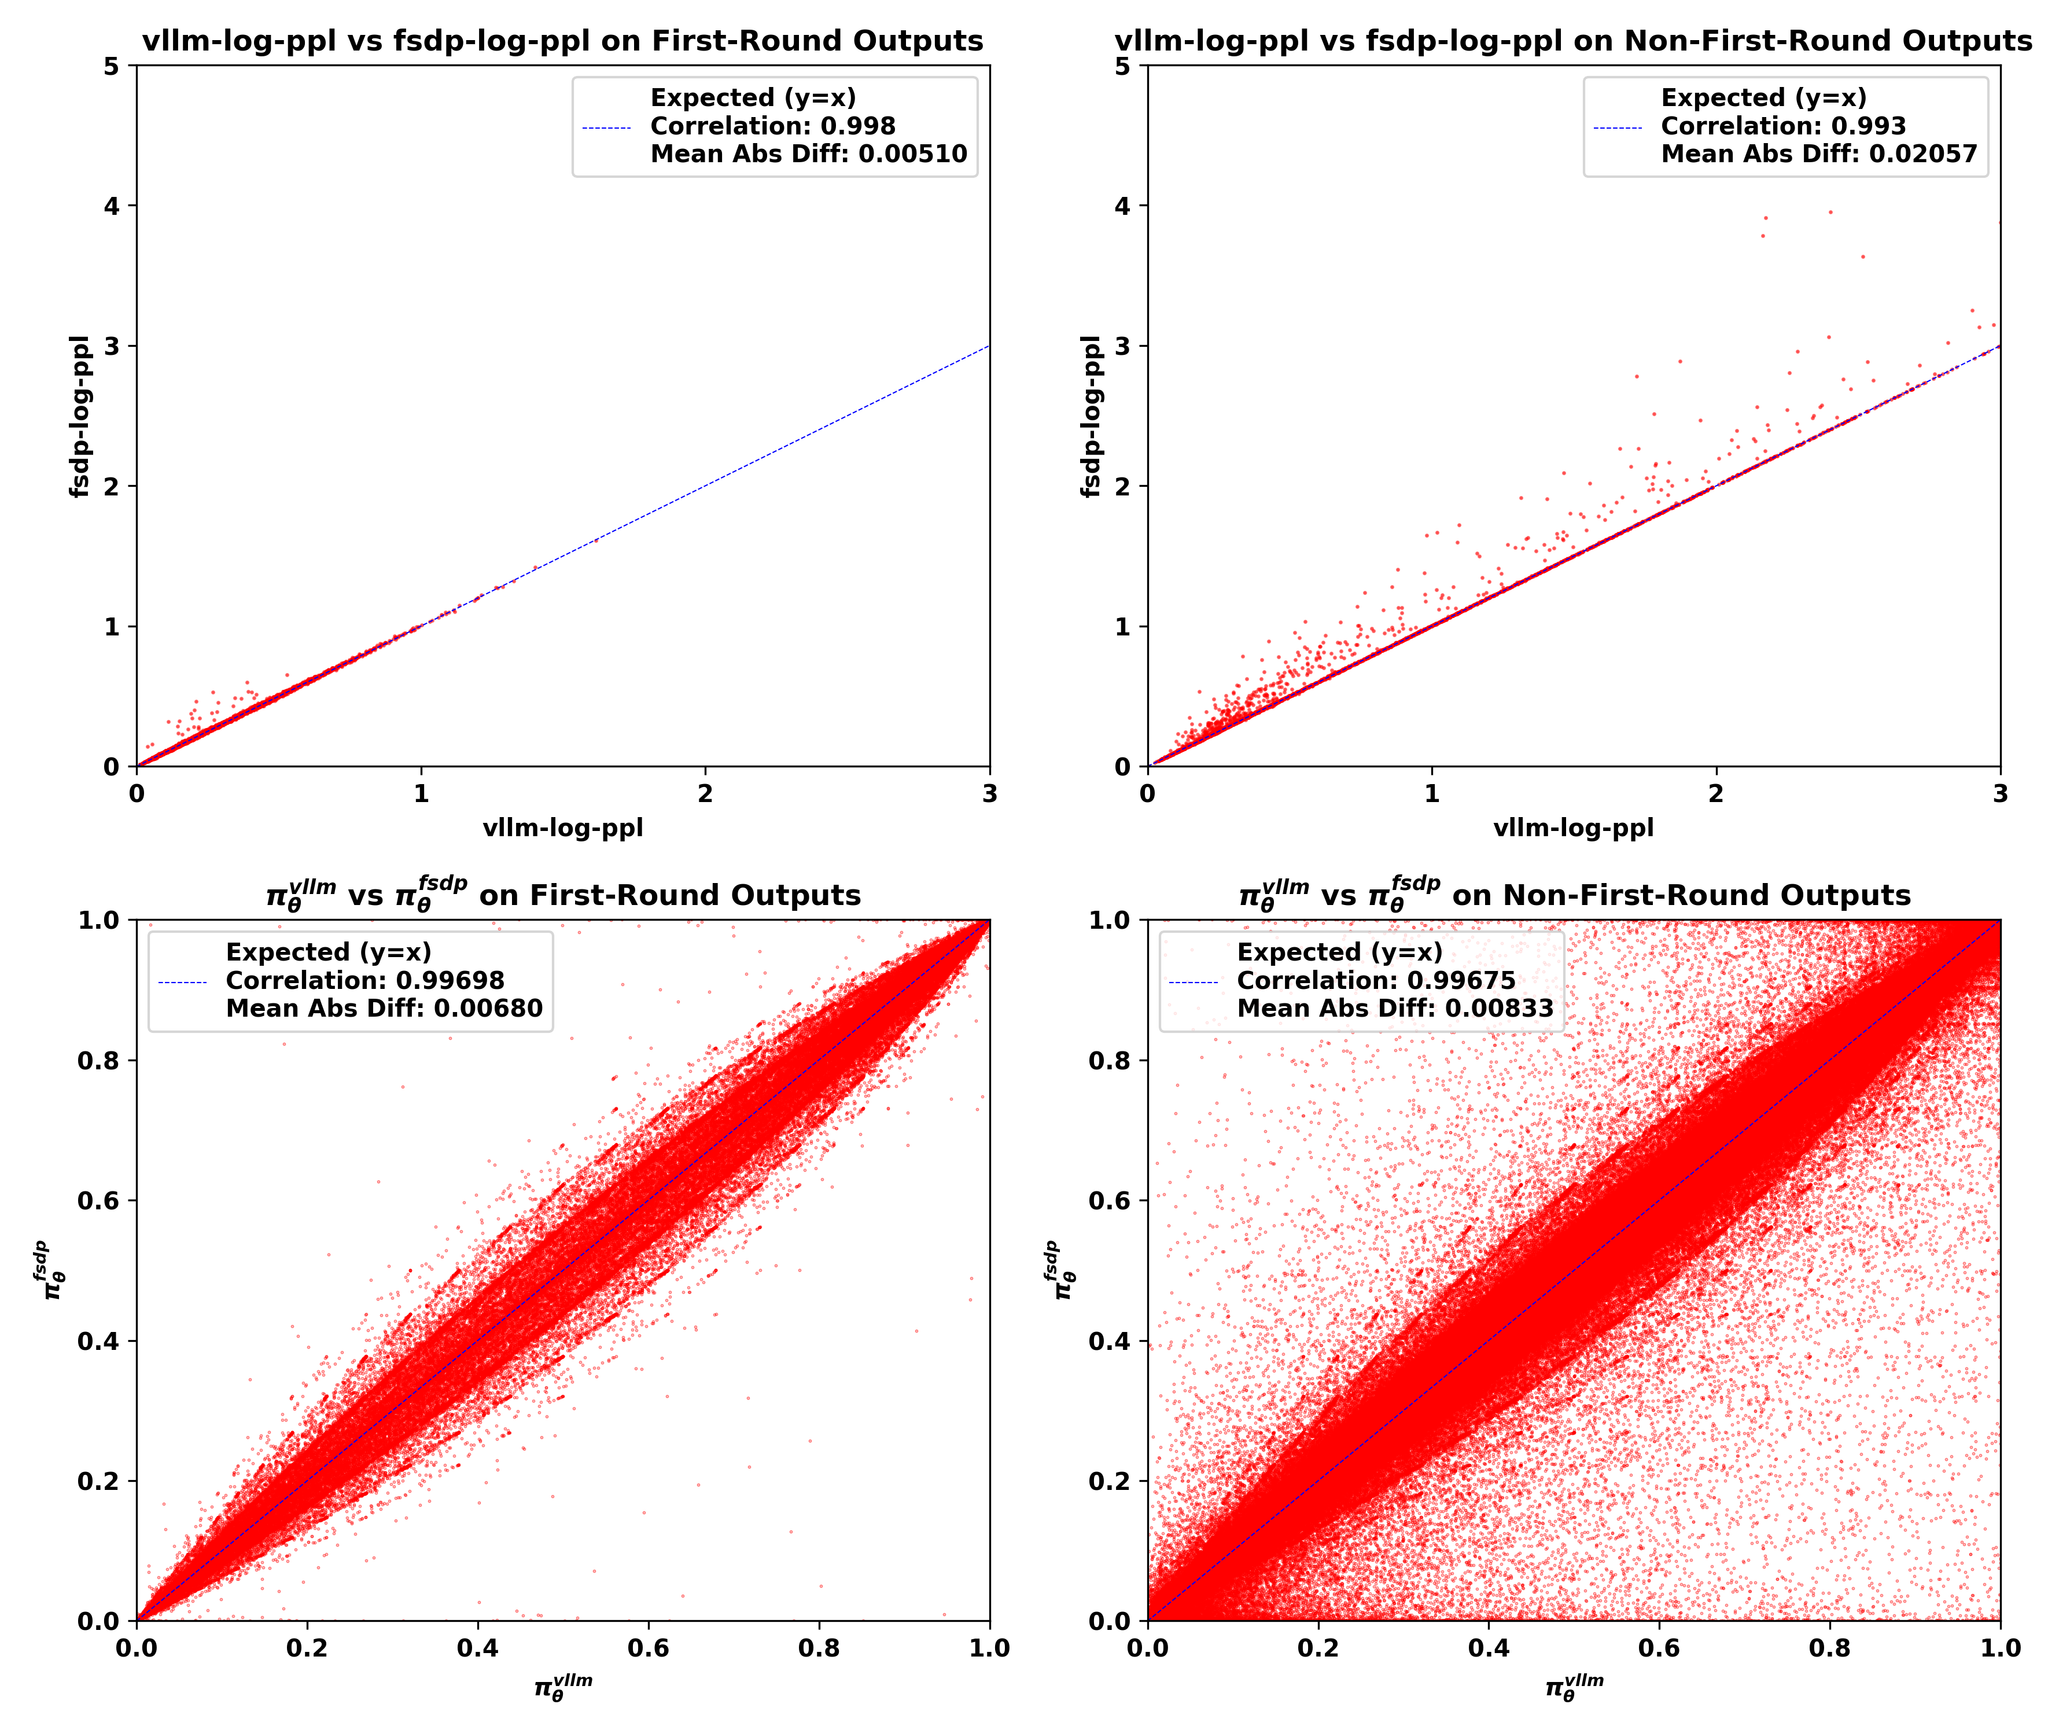
\includegraphics[width=\linewidth,height=0.64\textheight,keepaspectratio]{figures/image-09.png}
\caption*{第 2 组首轮与非首轮输出的不匹配可视化（原文未编号）：\code{vllm-kl} $\in[10^{-3},2\times10^{-2}]$。}
\end{figure}


% source-block: 271211a5-58b7-807c-b2f5-db46f3b9cf4a (bulleted_list; source-index: 105)

\begin{itemize}

\item \textbf{第 3 组：}\code{vllm-kl} $\in[2\times10^{-2},10^{-1}]$ 的批次。

\end{itemize}

% source-block: 271211a5-58b7-8024-8265-c6f33580b3be (image; source-index: 106)

\begin{figure}[H]
\centering
% source-block: 271211a5-58b7-8024-8265-c6f33580b3be (image)
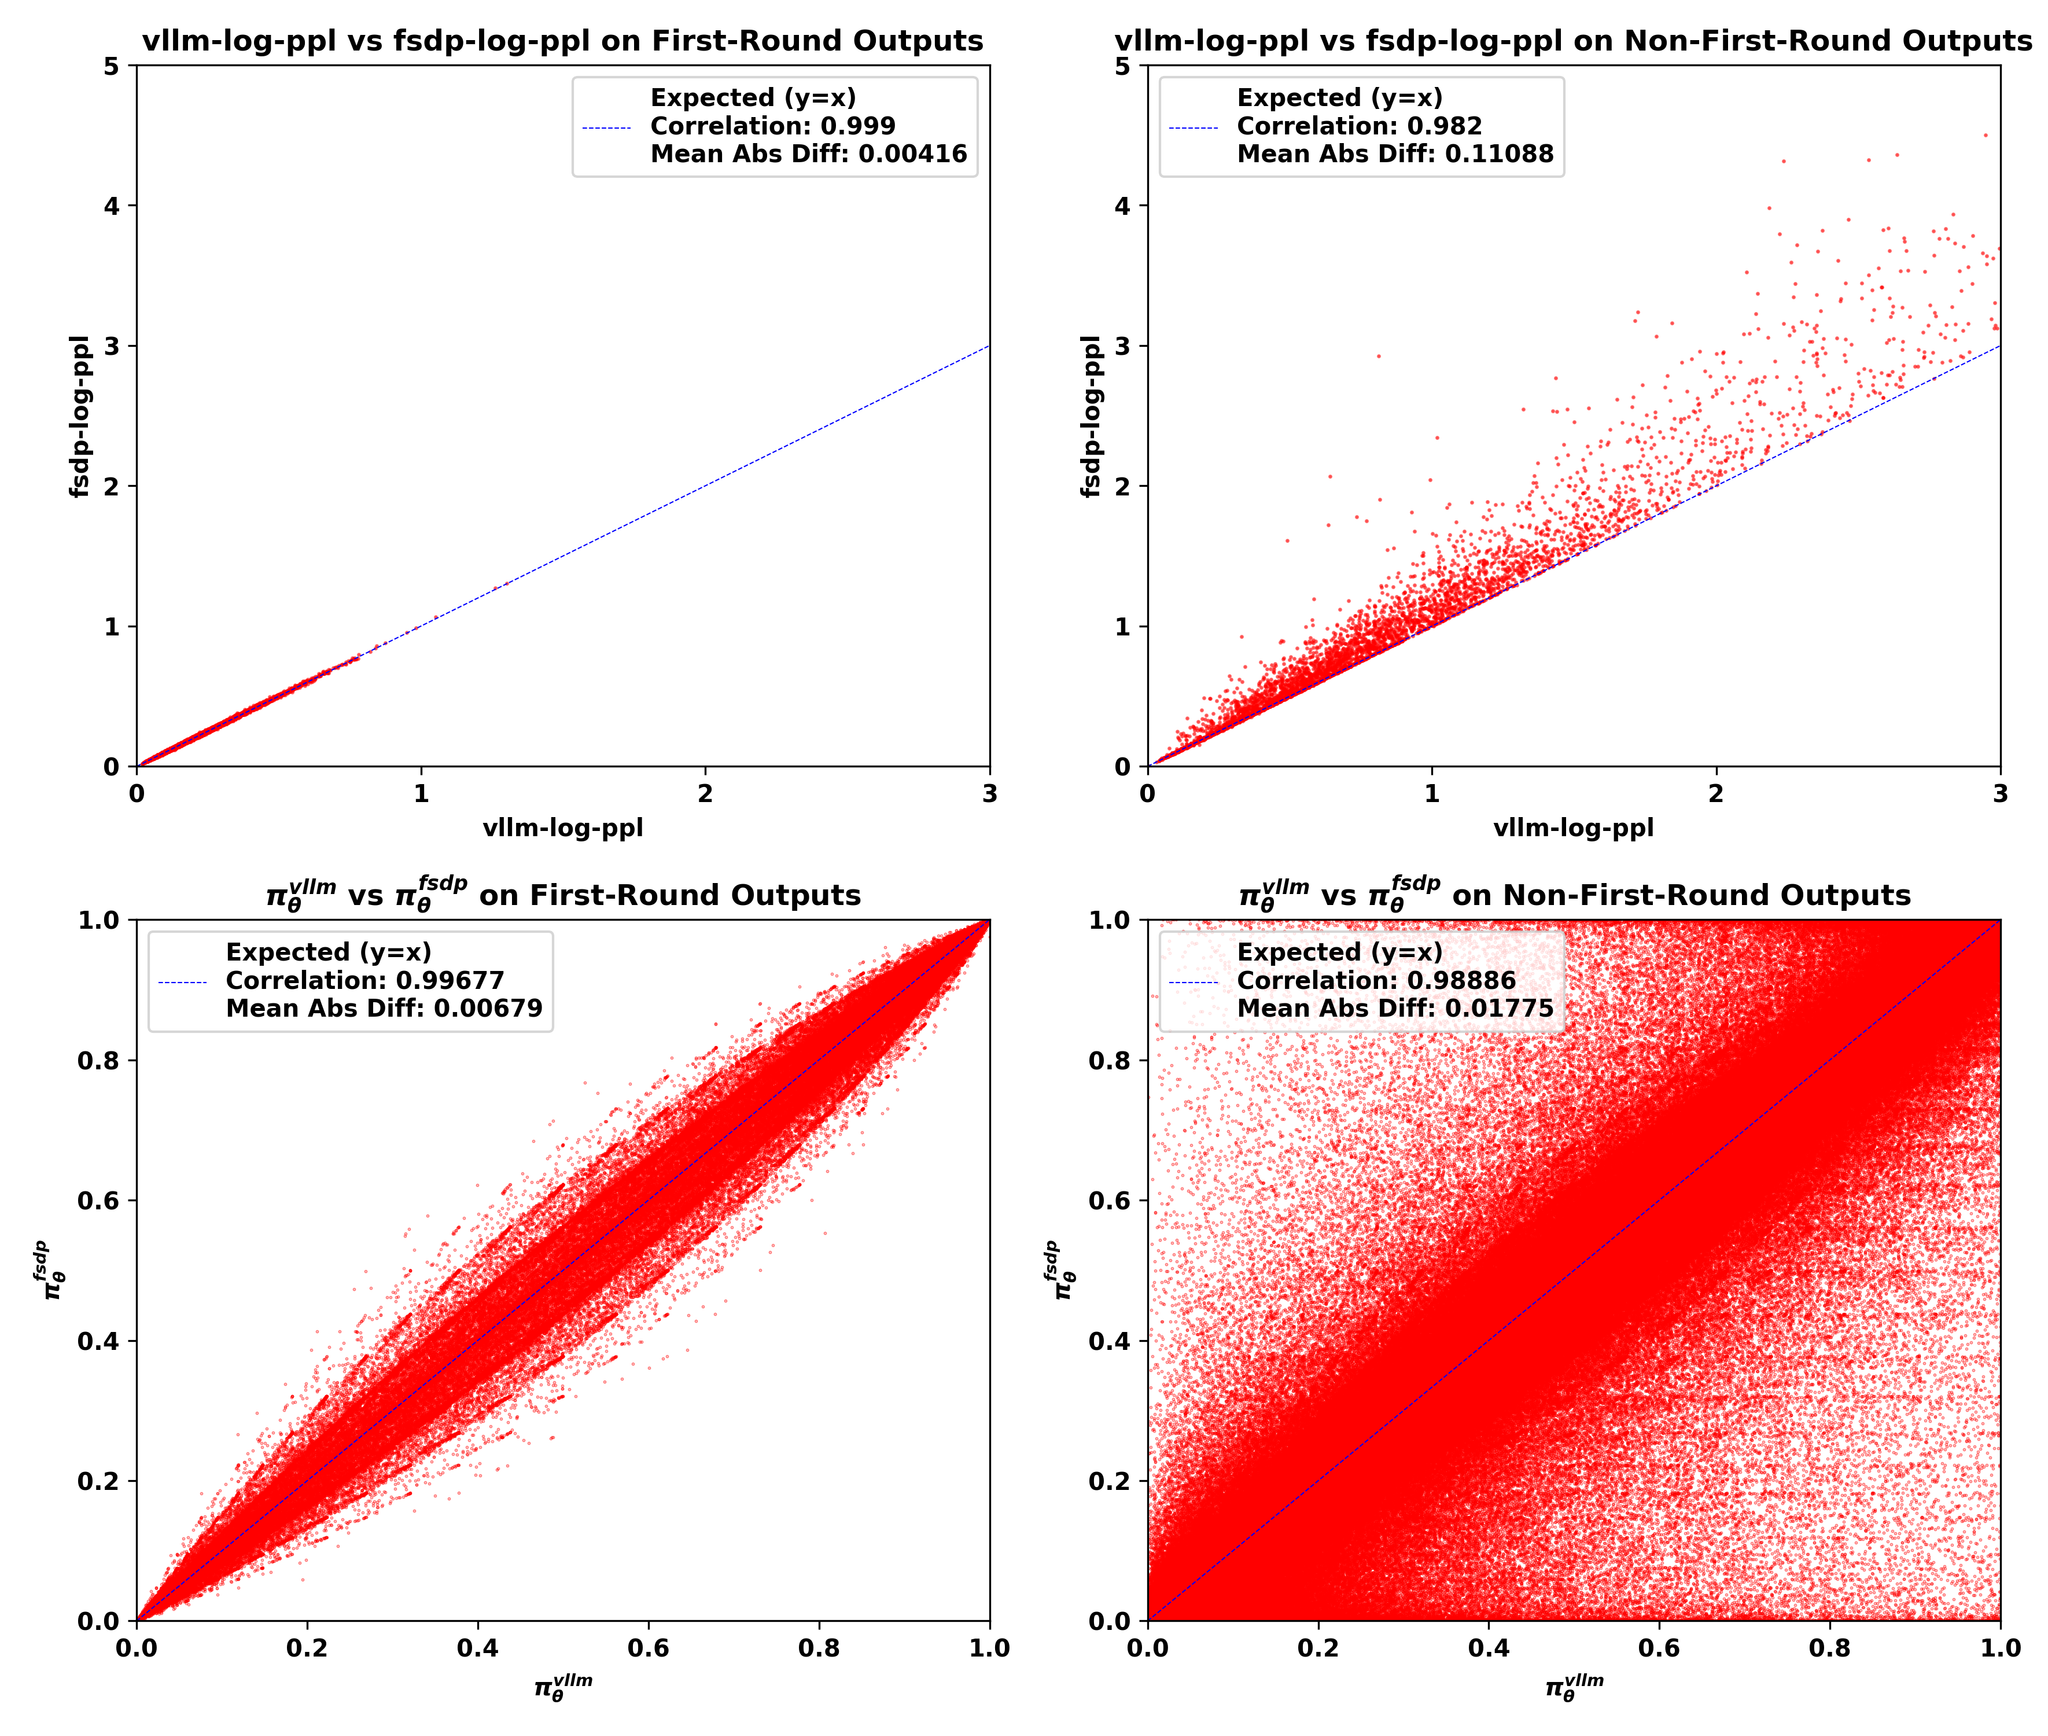
\includegraphics[width=\linewidth,height=0.64\textheight,keepaspectratio]{figures/image-10.png}
\caption*{第 3 组首轮与非首轮输出的不匹配可视化（原文未编号）：\code{vllm-kl} $\in[2\times10^{-2},10^{-1}]$。}
\end{figure}


% source-block: 271211a5-58b7-80e8-bb59-d8c2c4839f75 (text; source-index: 107)

从可视化结果可以观察到：


% source-block: 271211a5-58b7-80d4-bd8f-c072e9833bd0 (numbered_list; source-index: 108)

\begin{enumerate}

\item 非首轮输出的 \code{vllm-log-ppl} 通常大于首轮输出，说明模型面对不熟悉的分布外上下文时，会采样更多低概率词元。

% source-block: 271211a5-58b7-80da-9a4f-f339c3272a45 (numbered_list; source-index: 109)

\item 不匹配主要发生在非首轮输出中：与首轮输出相比，FSDP 与 vLLM 策略之间在对数困惑度和词元概率上的平均绝对差都更大，皮尔逊相关系数也更低。

% source-block: 271211a5-58b7-80b7-9b90-e3adee7c73c7 (numbered_list; source-index: 110)

\item 随着 \code{vllm-kl} 增大，训练与推理不匹配的恶化主要发生在非首轮输出。

% source-block: 271211a5-58b7-80ed-83ee-dd914cdf139e (numbered_list; source-index: 111)

\item 不匹配始终表现为 \code{fsdp-log-ppl} 大于 \code{vllm-log-ppl}，表明 FSDP 引擎产生了更极端的低概率词元。

\end{enumerate}

% source-block: 277211a5-58b7-80b6-9438-f97089a3b349 (divider; source-index: 112)

% source-block: 277211a5-58b7-805b-b021-d722c4d2eb3c (sub_sub_header; source-index: 113)

\hypertarget{src-277211a5-58b7-805b-b021-d722c4d2eb3c}{}
\subsubsection*{3.4.2 工具调用越多，训练越不稳定}


% source-block: 277211a5-58b7-803e-a52c-f2b1fd47d9f1 (text; source-index: 114)

下面的实验也表明，分布外工具响应会加剧训练与推理不匹配及训练不稳定性。我们在 H20 GPU 上，以 Qwen3-14B-Base 为基础模型开展异策略 GRPO 实验，设置 \code{clip higher=0.28}，并使用 4 个小批次。单条轨迹中工具调用次数的上限，即超参数 \code{max_tool_turn}，分别设为 20 和 100。图 5 和图 6 展示了结果：随着工具调用次数增多，训练更早崩溃；崩溃时，各次实验均观察到了梯度爆炸与 \code{vllm-kl} 爆炸。


% source-block: 277211a5-58b7-80fc-844d-edb200c466dc (image; source-index: 115)

\begin{figure}[H]
\centering
% source-block: 277211a5-58b7-80fc-844d-edb200c466dc (image)
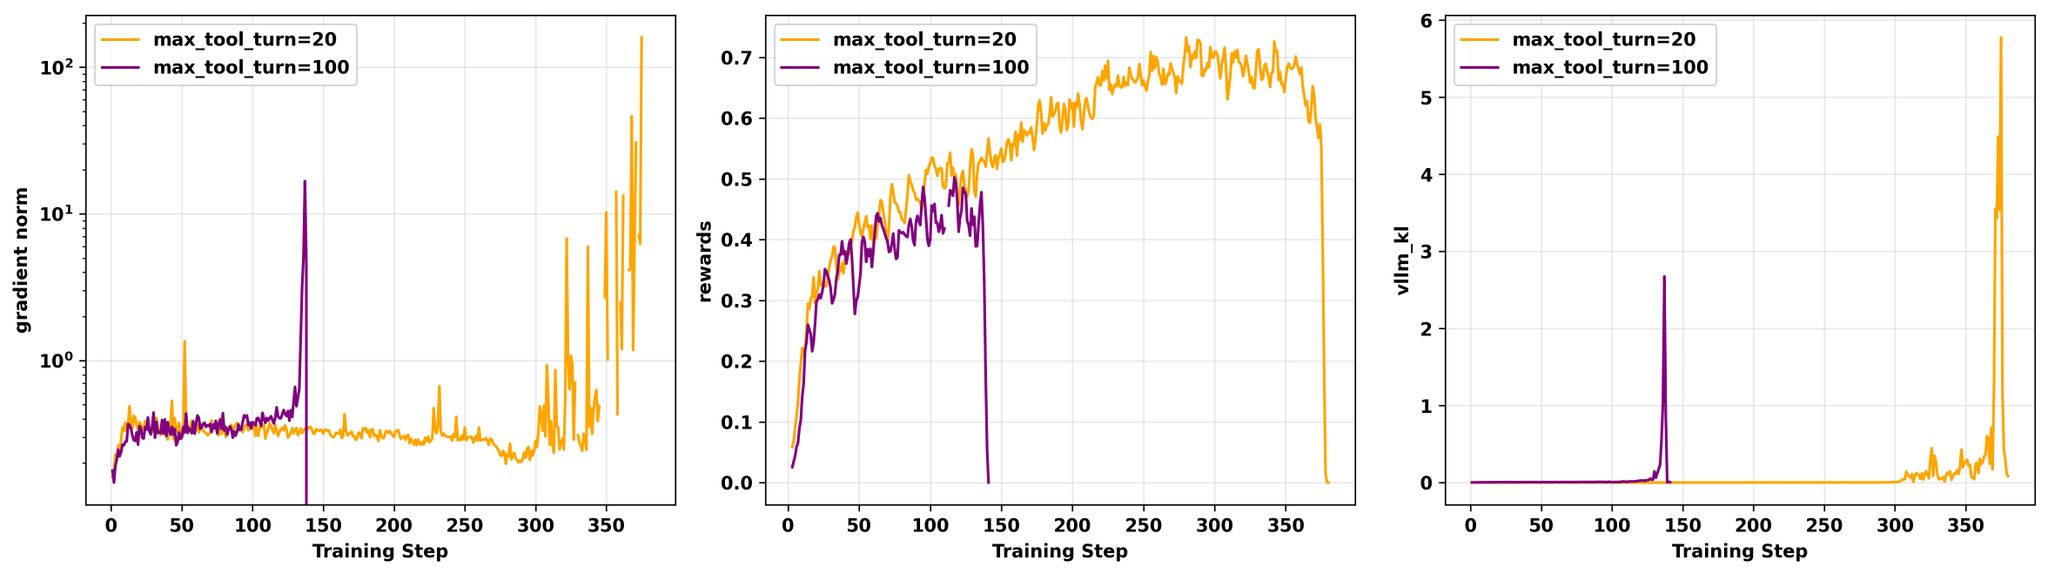
\includegraphics[width=\linewidth,height=0.64\textheight,keepaspectratio]{figures/image-11.jpg}
\caption*{\textbf{图 5。}不同 \code{max_tool_turn} 设置下，异策略 GRPO 的梯度范数（左）、奖励（中）与 \code{vllm-kl}（右）。均在 H20 上，以 Qwen3-14B-Base 为基础模型，设置 \code{clip higher=0.28}，使用 4 个小批次。}
\end{figure}


% source-block: 277211a5-58b7-80ed-902c-f6a8bd68c885 (image; source-index: 116)

\begin{figure}[H]
\centering
% source-block: 277211a5-58b7-80ed-902c-f6a8bd68c885 (image)
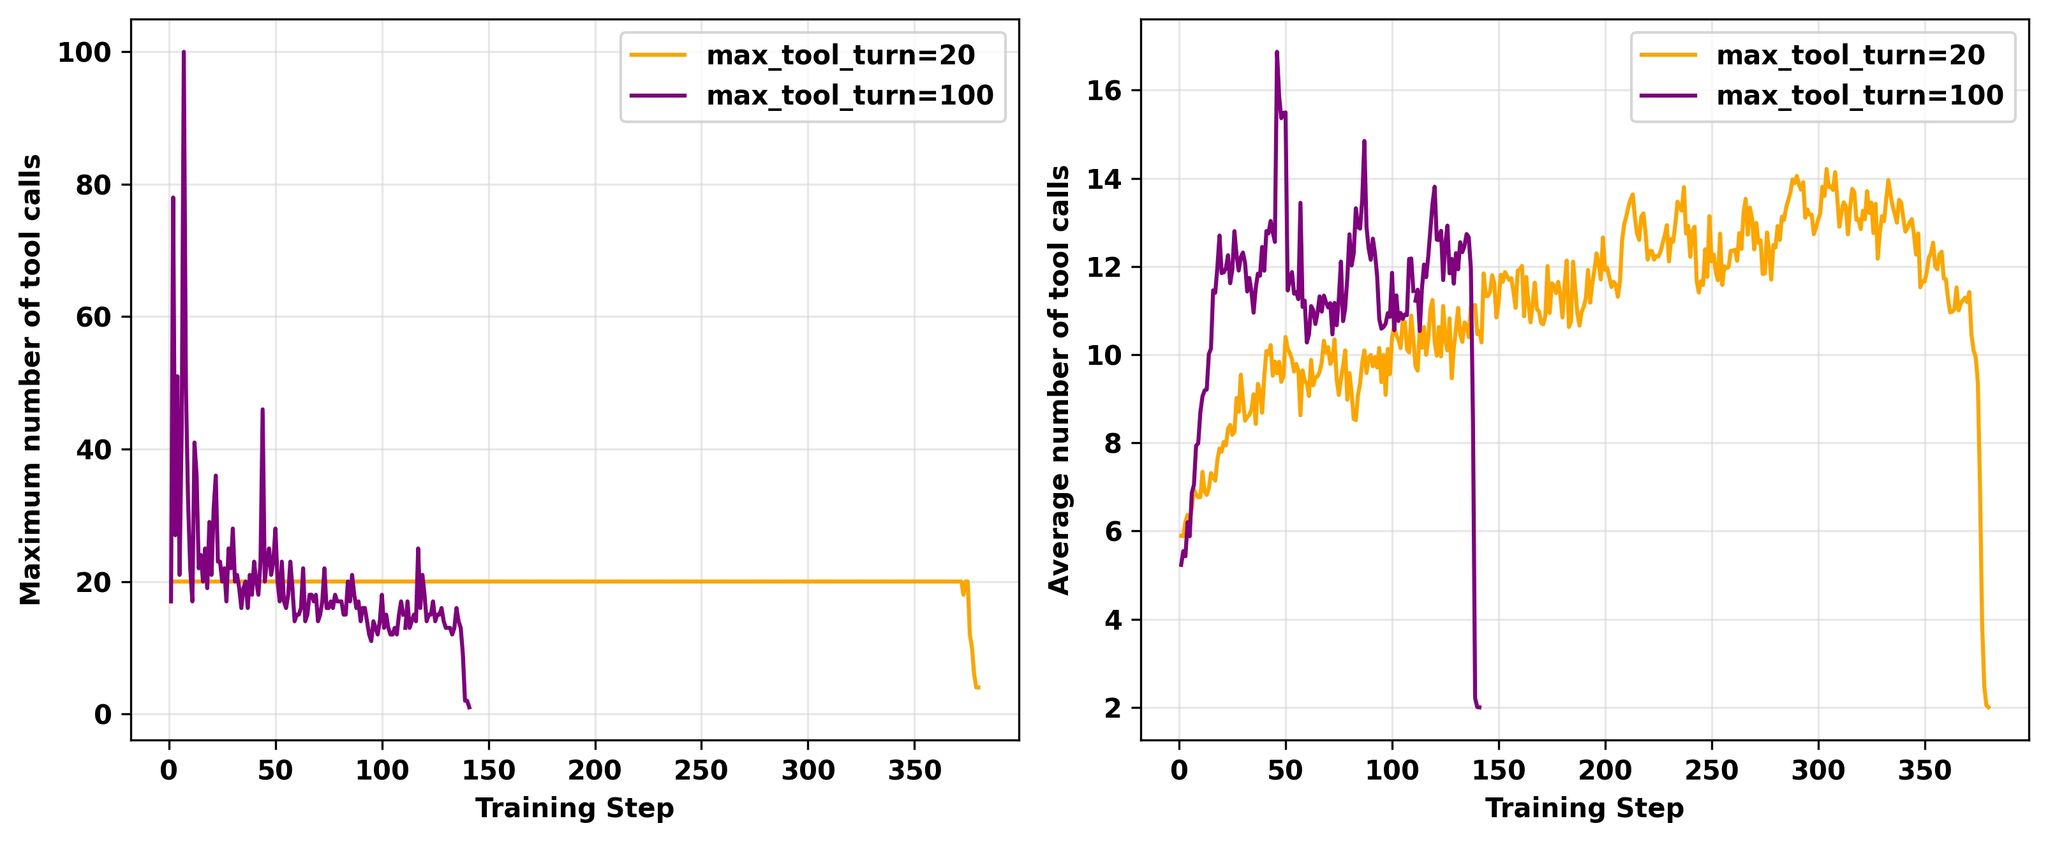
\includegraphics[width=\linewidth,height=0.64\textheight,keepaspectratio]{figures/image-12.jpg}
\caption*{\textbf{图 6。}不同 \code{max_tool_turn} 设置下，异策略 GRPO 的最大工具调用次数（左）与平均工具调用次数（右）。均在 H20 上，以 Qwen3-14B-Base 为基础模型，设置 \code{clip higher=0.28}，使用 4 个小批次。}
\end{figure}


% source-block: 277211a5-58b7-8084-89d4-ea00c3bdbc3b (divider; source-index: 117)

% source-block: 271211a5-58b7-80c9-ad90-f8aa1353bfe1 (sub_header; source-index: 118)

\hypertarget{src-271211a5-58b7-80c9-ad90-f8aa1353bfe1}{}
\subsection*{3.5 环境因素：硬件的关键作用}
\phantomsection
\addcontentsline{toc}{subsection}{3.5 环境因素：硬件的关键作用}


% source-block: 271211a5-58b7-8008-a5ba-ec1353923d67 (text; source-index: 119)

最后，我们发现物理硬件是一个关键变量。\textbf{完全相同的代码与模型，在不同 GPU 硬件上产生的不匹配程度差异巨大。}为评估硬件差异，我们在相同代码环境与超参数下运行同策略算法，只更换用于推理和训练的 GPU。图 7 分别展示了 L20、H20 和 A100 上的训练动态。


% source-block: 271211a5-58b7-807d-b017-dc3d1d908ff8 (image; source-index: 120)

\begin{figure}[H]
\centering
% source-block: 271211a5-58b7-807d-b017-dc3d1d908ff8 (image)
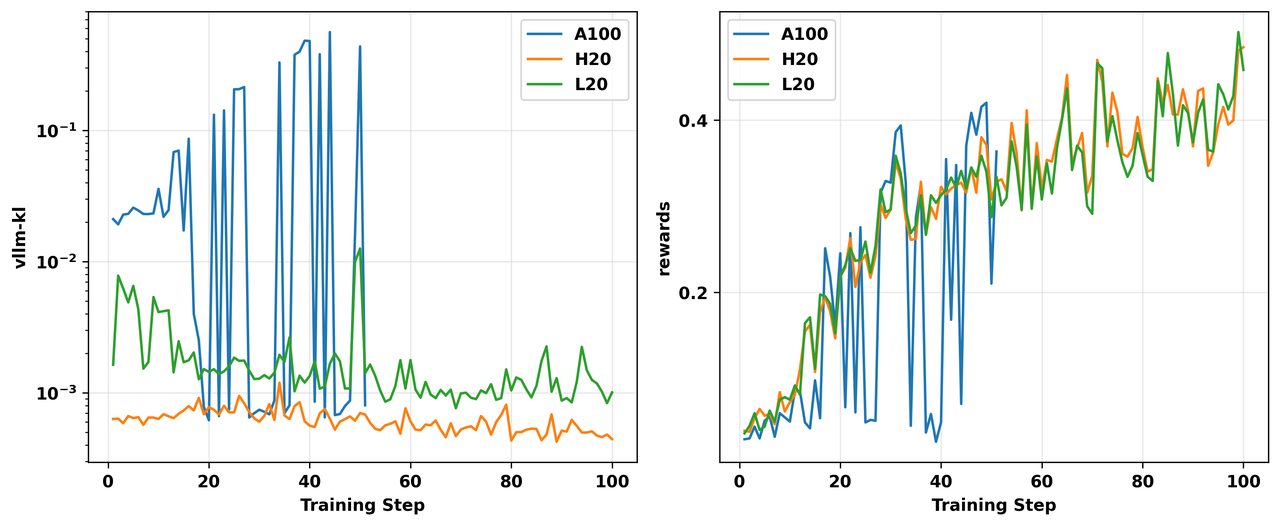
\includegraphics[width=\linewidth,height=0.64\textheight,keepaspectratio]{figures/image-13.png}
\caption*{\textbf{图 7。}不同 GPU 上，同策略 GRPO 实验的 \code{vllm-kl}（左）与奖励（右）。所有实验均使用相同代码与环境。}
\end{figure}


% source-block: 271211a5-58b7-8016-87f5-c640d0f8d5f0 (text; source-index: 121)

在我们的实验中，\code{vllm-kl} 的量级基本满足 \textbf{H20 $<$ L20 $<$ A100}。具体而言，H20 通常为 $5\times10^{-4}$ 至 $10^{-3}$，L20 约为 $10^{-3}$ 至 $10^{-2}$，A100 则主要处于 $10^{-2}$ 至 $1$。A100 上严重的训练与推理不匹配使正常训练难以进行，奖励曲线高度不稳定。


% source-block: 2a8211a5-58b7-8062-8a6a-ed98d6c13b5f (text; source-index: 122)

我们发现，在 A100 GPU 实验中，关闭 vLLM 的级联注意力（cascade attention）尤其有助于减小不匹配。相关结果见第 4.2.4 节。


% source-block: 271211a5-58b7-8077-a02a-f7bad00d87a1 (text; source-index: 123)

最有说服力的证据来自一次恢复实验：我们将 L20 上失败实验的检查点转移到 H20 GPU 上继续训练（见图 8），训练立即稳定并恢复，说明硬件对该问题具有直接且显著的影响。


% source-block: 271211a5-58b7-8039-b3b1-ddc62d10f463 (image; source-index: 124)

\begin{figure}[H]
\centering
% source-block: 271211a5-58b7-8039-b3b1-ddc62d10f463 (image)
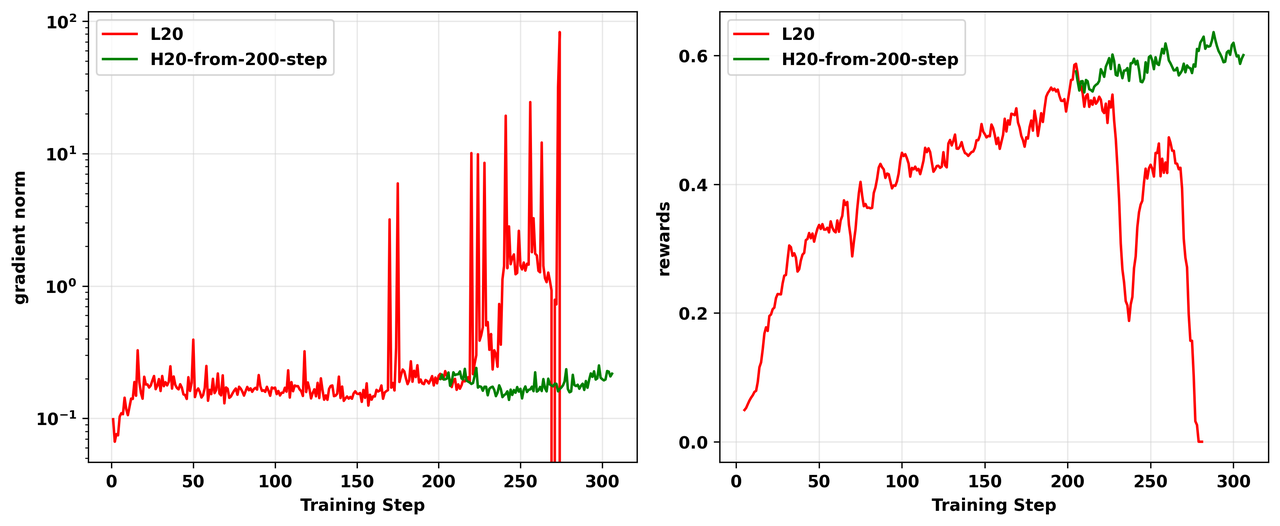
\includegraphics[width=\linewidth,height=0.64\textheight,keepaspectratio]{figures/image-14.png}
\caption*{\textbf{图 8。}L20 与 H20 上同策略 GRPO 实验的梯度范数（左）和奖励（右）。H20 实验（绿线）从失败 L20 实验（红线）的第 200 步检查点启动。}
\end{figure}


% source-block: 277211a5-58b7-8060-a17d-d48fb6c48d1e (divider; source-index: 125)

% source-block: 271211a5-58b7-8029-a918-f29c6ca7198d (sub_header; source-index: 126)

\hypertarget{src-271211a5-58b7-8029-a918-f29c6ca7198d}{}
\subsection*{3.6 不匹配并非静态：由优化驱动的恶性循环}
\phantomsection
\addcontentsline{toc}{subsection}{3.6 不匹配并非静态：由优化驱动的恶性循环}


% source-block: 271211a5-58b7-802e-a9bf-ea88ac4a7010 (text; source-index: 127)

人们可能以为，训练与推理不匹配是硬件和软件栈的静态属性。但下面的“批次过滤”（batch-filter）实验表明，\textbf{不匹配与训练动态及模型状态相互耦合。}


% source-block: 271211a5-58b7-8087-ab3d-c93b7634665c (text; source-index: 128)

在批次过滤实验中，每个训练步采用如下更新策略：若采集批次的 \code{vllm-kl} 大于阈值，则跳过该批次上的参数更新，因为这类更新容易引发训练崩溃；随后直接进入下一步，继续收集数据，直到取得 \code{vllm-kl} 低于阈值的批次，再更新模型。


% source-block: 271211a5-58b7-80ff-9032-c093eab4840b (text; source-index: 129)

该实验的逻辑是：如果不匹配程度完全独立于模型输出分布和训练动态，那么不同训练步中的 \code{vllm-kl} 应具有相同分布。然而，图 9 表明，一旦模型进入某种状态，就开始持续生成高度不匹配的批次，使训练实际上陷入停滞。再结合其他实验中 \code{vllm-kl} 与 \code{fsdp-ppl} 螺旋式攀升的现象（图 10），这些证据指向一个危险的反馈回路。


% source-block: 271211a5-58b7-80db-ad92-f9d2ded4a453 (image; source-index: 130)

\begin{figure}[H]
\centering
% source-block: 271211a5-58b7-80db-ad92-f9d2ded4a453 (image)
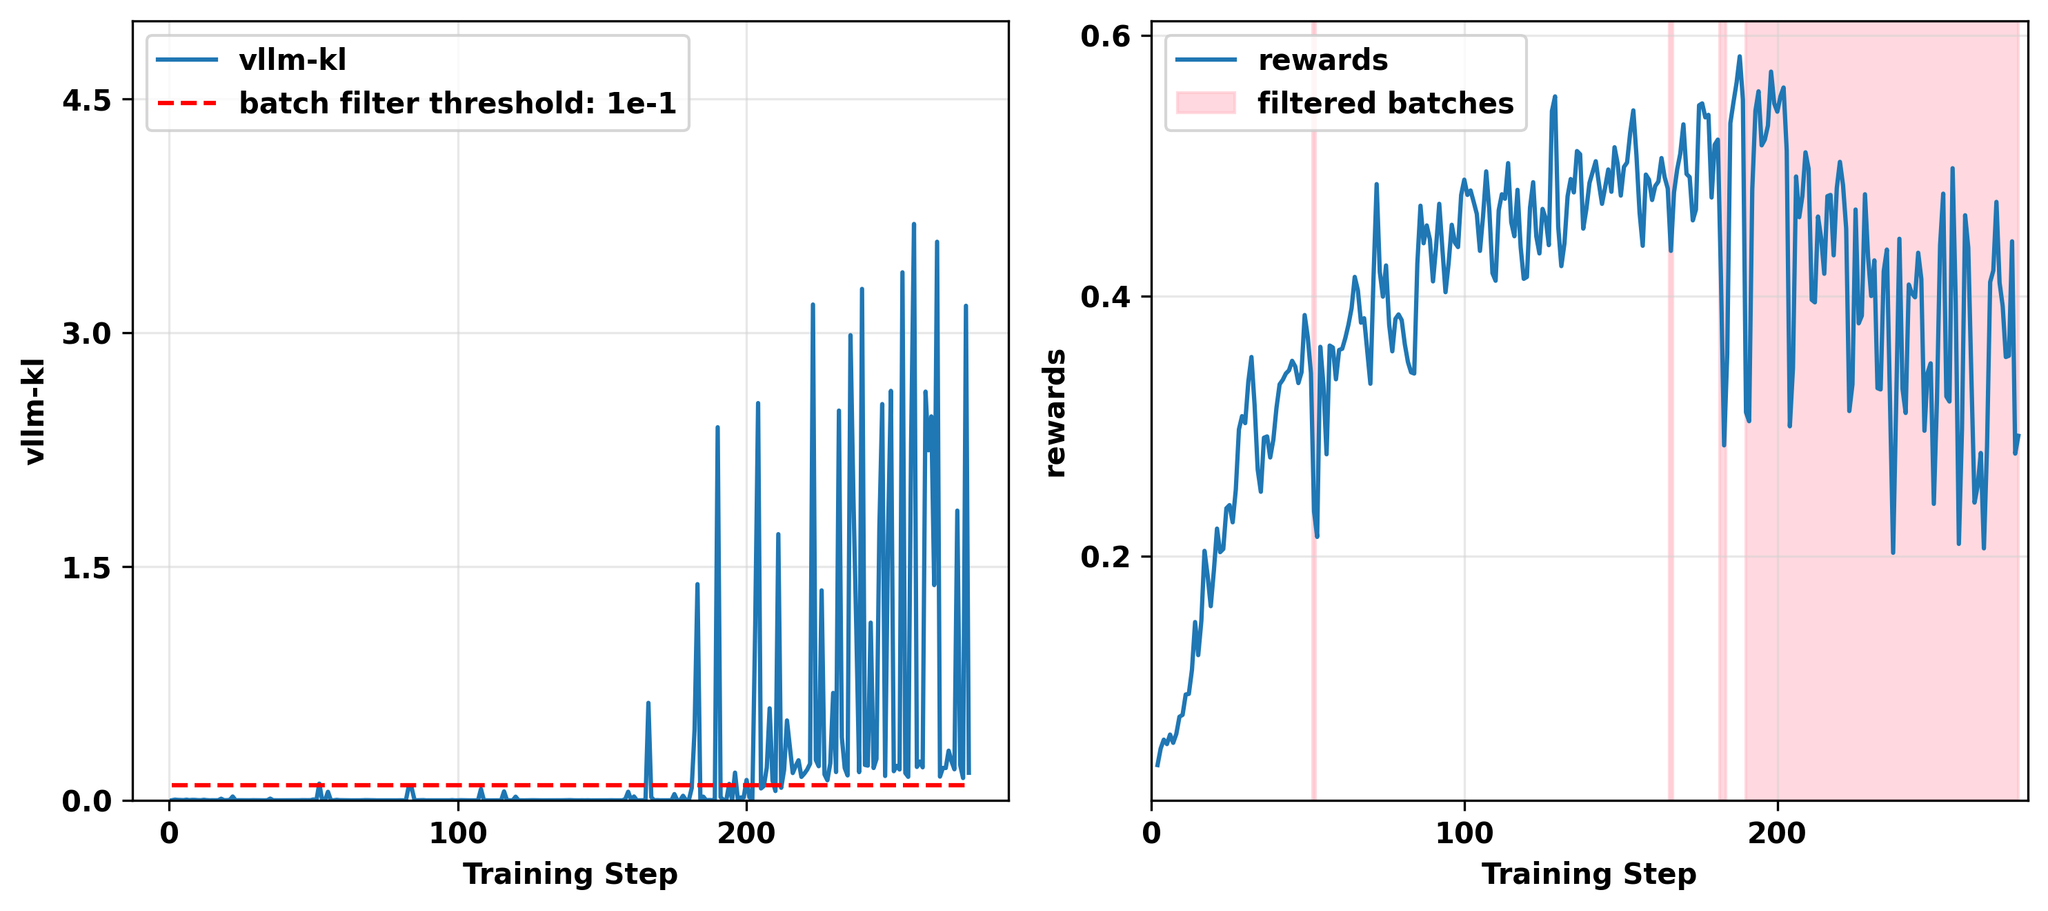
\includegraphics[width=\linewidth,height=0.64\textheight,keepaspectratio]{figures/image-15.png}
\caption*{\textbf{图 9。}同策略“批次过滤”实验的 \code{vllm-kl}（左）与奖励（右）。过滤阈值设为 0.1；批次被过滤的训练步用粉色标出。}
\end{figure}


% source-block: 271211a5-58b7-80eb-8c3c-fc81889860ed (image; source-index: 131)

\begin{figure}[H]
\centering
% source-block: 271211a5-58b7-80eb-8c3c-fc81889860ed (image)
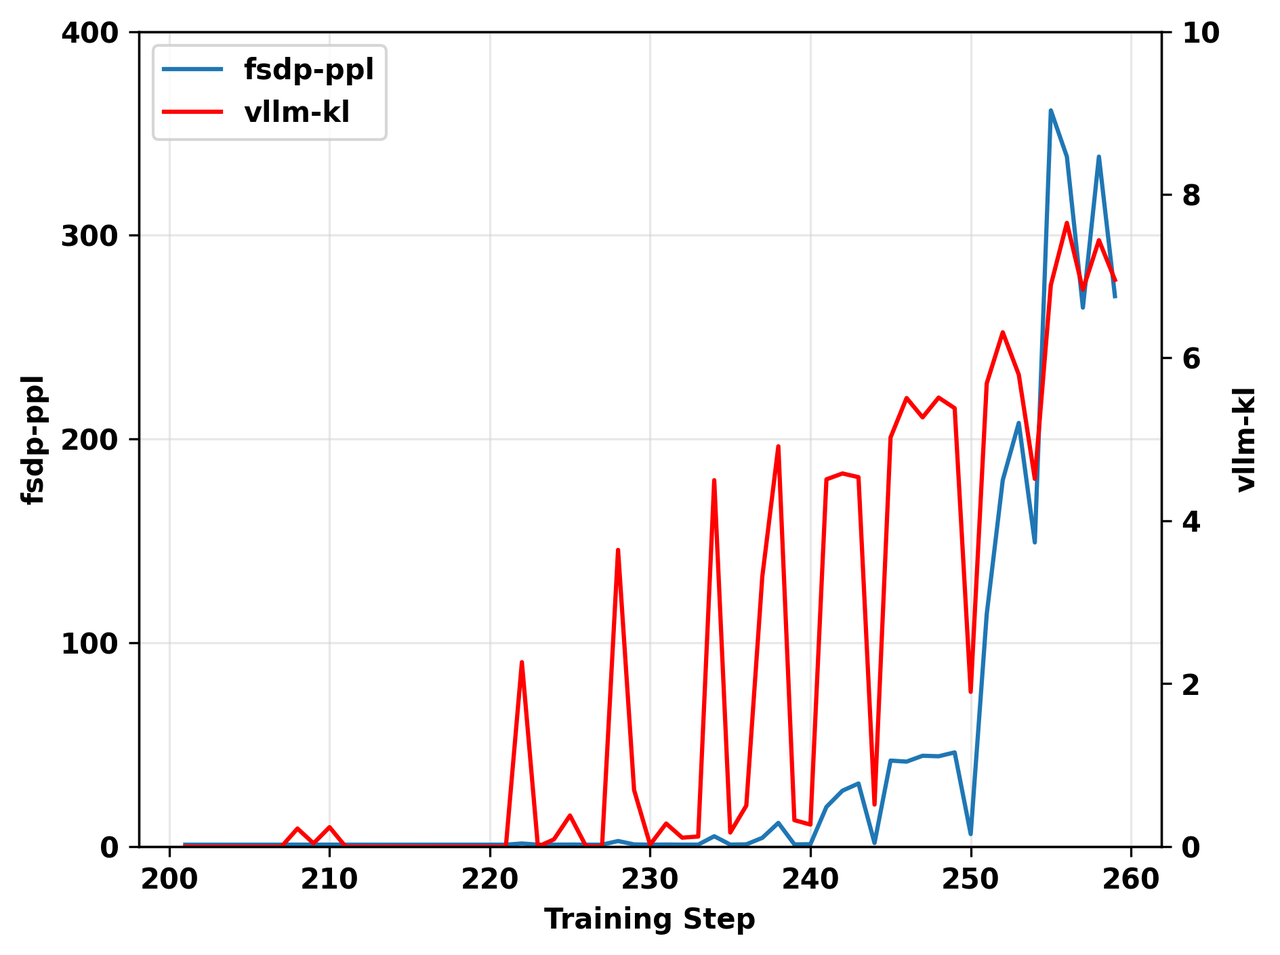
\includegraphics[width=\linewidth,height=0.64\textheight,keepaspectratio]{figures/image-16.png}
\caption*{\textbf{图 10。}一次同策略实验中，\code{vllm-kl} 与 \code{fsdp-ppl} 随训练步数的变化。两条曲线呈现相互关联、螺旋式上升的模式。}
\end{figure}


% source-block: 271211a5-58b7-8003-8533-ec98b0d66201 (text; source-index: 132)

\textbf{我们推测，这是以下两阶段级联失效造成的：}


% source-block: 271211a5-58b7-80ff-81ad-fa6e9105dbf4 (numbered_list; source-index: 133)

\begin{enumerate}

\item \textbf{阶段 1：数值敏感性增加。}强化学习优化器将模型权重推入 \code{bfloat16} 相对精度较低的数值范围，例如非常小或非常大的值。\footnote{译注：此处忠实保留作者的机制假设。对普通正规数，BF16 的相对间隔大致固定；极端值还可能涉及上溢、下溢或次正规数。因此，这段表述不应被当作已由本文实验直接验证的浮点数性质。}

% source-block: 271211a5-58b7-8080-8d52-fb6ef5e4adc4 (numbered_list; source-index: 134)

\item \textbf{阶段 2：内核驱动的误差放大。}这些初始的微小 \code{bfloat16} 量化误差进入 vLLM 与 FSDP 的不同内核实现。不同的计算顺序充当非线性放大器，使很小的初始偏差不断累积，最终造成 logits 的巨大差异。

\end{enumerate}

% source-block: 271211a5-58b7-80d5-a007-e96da4174eb1 (text; source-index: 135)

由此形成恶性反馈回路：不匹配产生有偏且噪声较大的梯度；这些梯度可能进一步将参数推向数值敏感区域；这又加剧下一次迭代的不匹配，直至系统崩溃。


% source-block: 277211a5-58b7-80cc-bdf2-edc86beb5fbc (divider; source-index: 136)

% Chinese translation assembled from source/blocks.json.

% See source/translation.py for the translation and source/build_tex.py for assembly.

% source-block: 271211a5-58b7-80b8-9a51-c4976dca1254 (header; source-index: 137)

\hypertarget{src-271211a5-58b7-80b8-9a51-c4976dca1254}{}
\section*{4. 缓解训练与推理不匹配的尝试}
\phantomsection
\addcontentsline{toc}{section}{4. 缓解训练与推理不匹配的尝试}


% source-block: 271211a5-58b7-8025-aee7-c19ceda8ac80 (text; source-index: 138)

下面列出我们尝试过的缓解方法。其中有些有效，有些没有奏效。


% source-block: 271211a5-58b7-80f7-beba-e43453ed1380 (sub_header; source-index: 139)

\hypertarget{src-271211a5-58b7-80f7-beba-e43453ed1380}{}
\subsection*{4.1 未奏效的尝试}
\phantomsection
\addcontentsline{toc}{subsection}{4.1 未奏效的尝试}


% source-block: 271211a5-58b7-80c3-96aa-ed277ca67b21 (sub_sub_header; source-index: 140)

\hypertarget{src-271211a5-58b7-80c3-96aa-ed277ca67b21}{}
\subsubsection*{4.1.1 使用 FP32 语言模型输出头}


% source-block: 271211a5-58b7-802d-a418-e2b9da375651 (text; source-index: 141)

受 \href{https://arxiv.org/abs/2506.13585}{MiniMax-M1 技术报告}和博客\href{https://fengyao.notion.site/off-policy-rl}{《高效的强化学习框架暗中将训练变成了异策略强化学习》}启发，我们修改 vLLM，将 \code{lm_head} 转为 FP32 精度。然而，修改后不匹配仍然存在，模型崩溃依旧无法避免。图 11 对比了 L20 上使用 BF16 \code{lm_head} 的失败同策略实验，以及从该失败实验第 200 步恢复、改用 FP32 \code{lm_head} 的实验。两次实验最终都崩溃了，使用 FP32 \code{lm_head} 的实验仍出现了 \code{vllm-kl} 爆炸。


% source-block: 271211a5-58b7-80d3-98ac-fe024795f621 (image; source-index: 142)

\begin{figure}[H]
\centering
% source-block: 271211a5-58b7-80d3-98ac-fe024795f621 (image)
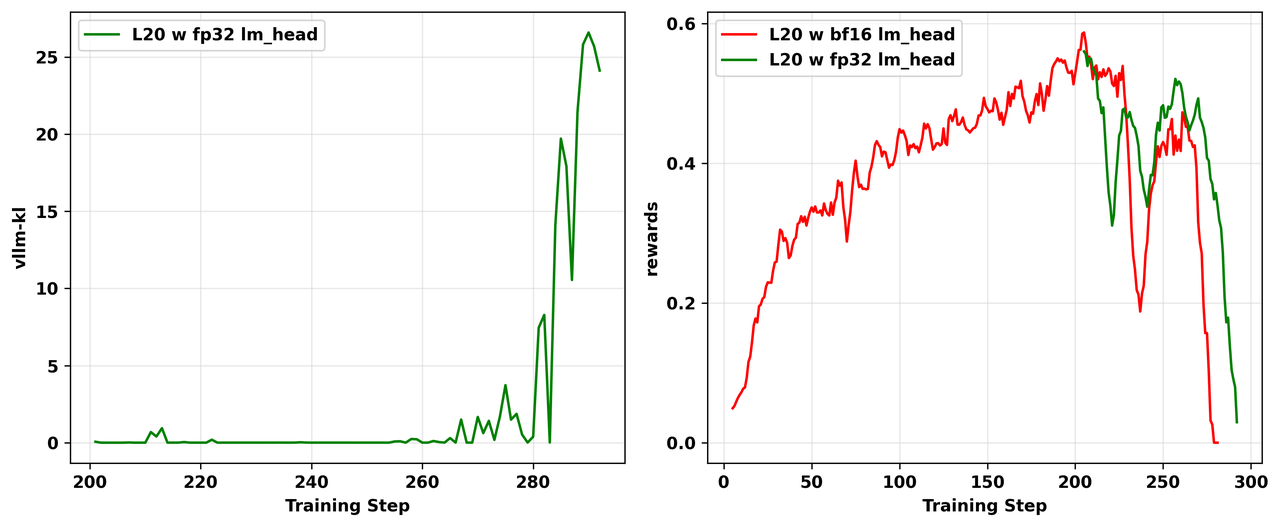
\includegraphics[width=\linewidth,height=0.64\textheight,keepaspectratio]{figures/image-17.png}
\caption*{\textbf{图 11。}vLLM 引擎中 \code{lm_head} 精度的消融实验。左：\code{vllm-kl}；右：训练奖励。使用 FP32 \code{lm_head} 的实验，从 BF16 \code{lm_head} 失败实验的第 200 步恢复。}
\end{figure}


% source-block: 277211a5-58b7-8065-8a78-def969cdd1ca (divider; source-index: 143)

% source-block: 271211a5-58b7-80ee-960c-f43a87c9177a (sub_sub_header; source-index: 144)

\hypertarget{src-271211a5-58b7-80ee-960c-f43a87c9177a}{}
\subsubsection*{4.1.2 关闭分块预填充}


% source-block: 271211a5-58b7-804e-b961-ec63fb9bf0a5 (text; source-index: 145)

我们还从第 4.1.1 节中使用 BF16 \code{lm_head} 的失败实验第 200 步恢复训练，尝试关闭\href{https://docs.vllm.ai/en/v0.4.2/models/performance.html}{分块预填充（chunked prefill）}，检验能否解决崩溃。图 12 表明，这一方法没有解决问题。


% source-block: 271211a5-58b7-8054-8c5b-d9ce67ee4d3d (image; source-index: 146)

\begin{figure}[H]
\centering
% source-block: 271211a5-58b7-8054-8c5b-d9ce67ee4d3d (image)
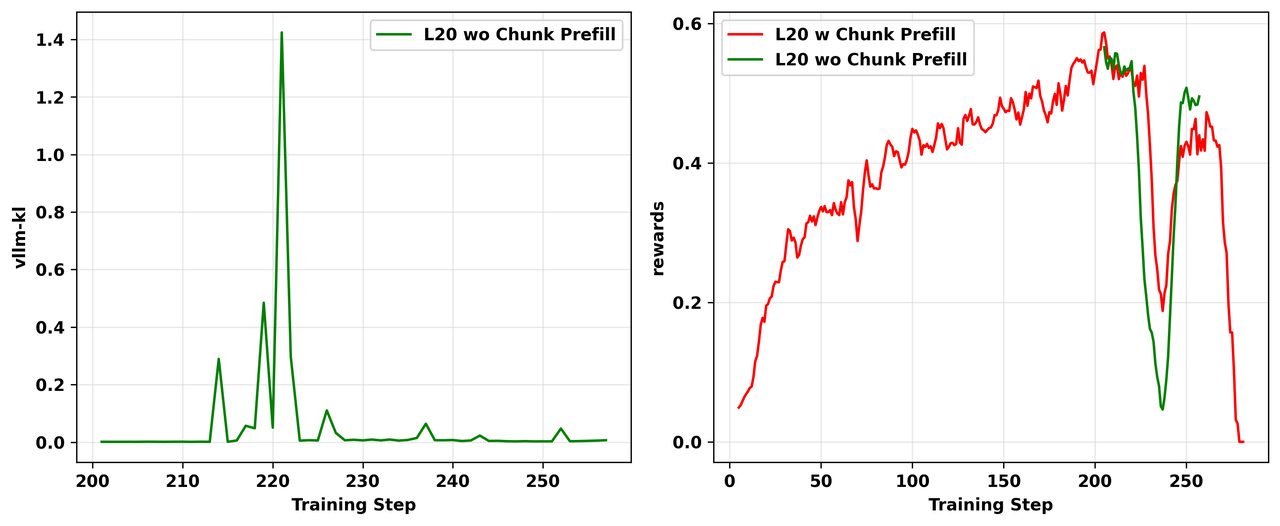
\includegraphics[width=\linewidth,height=0.64\textheight,keepaspectratio]{figures/image-18.png}
\caption*{\textbf{图 12。}分块预填充的消融实验。从此前启用分块预填充的失败实验第 200 步恢复训练，并关闭该功能。左：\code{vllm-kl}；右：训练奖励。}
\end{figure}


% source-block: 271211a5-58b7-8079-881a-cb3f4f1ef2c6 (sub_sub_header; source-index: 147)

\hypertarget{src-271211a5-58b7-8079-881a-cb3f4f1ef2c6}{}
\subsubsection*{4.1.3 启用 \texttt{enforce\_eager} 和 \texttt{free\_cache\_engine}}


% source-block: 271211a5-58b7-80f3-a489-f51061ca6f89 (text; source-index: 148)

\href{https://verl.readthedocs.io/en/latest/algo/dapo.html}{VeRL 的 DAPO 官方配方}提到，启用 CUDA Graph（\code{enforce_eager=False}，原文此处拼作 \code{enforce_eage}）可能导致模型性能下降。为研究它是否影响训练与推理不匹配，我们同时考虑另一个超参数 \code{free_cache_engine}，开展消融实验。

实验采用推理强化学习设置：在 H100 GPU 上，以 Qwen3-4B-Base 为基础模型运行同策略 GRPO，将 \code{enforce_eager} 与 \code{free_cache_engine} 分别设为 \code{True} 或 \code{False}，穷举四种组合，并在 AIME24 上评估。图 13 表明，调整这两个参数，对训练与推理不匹配以及测试性能均没有显著影响。


% source-block: 271211a5-58b7-8084-b459-d4cd5f78014f (image; source-index: 149)

\begin{figure}[H]
\centering
% source-block: 271211a5-58b7-8084-b459-d4cd5f78014f (image)
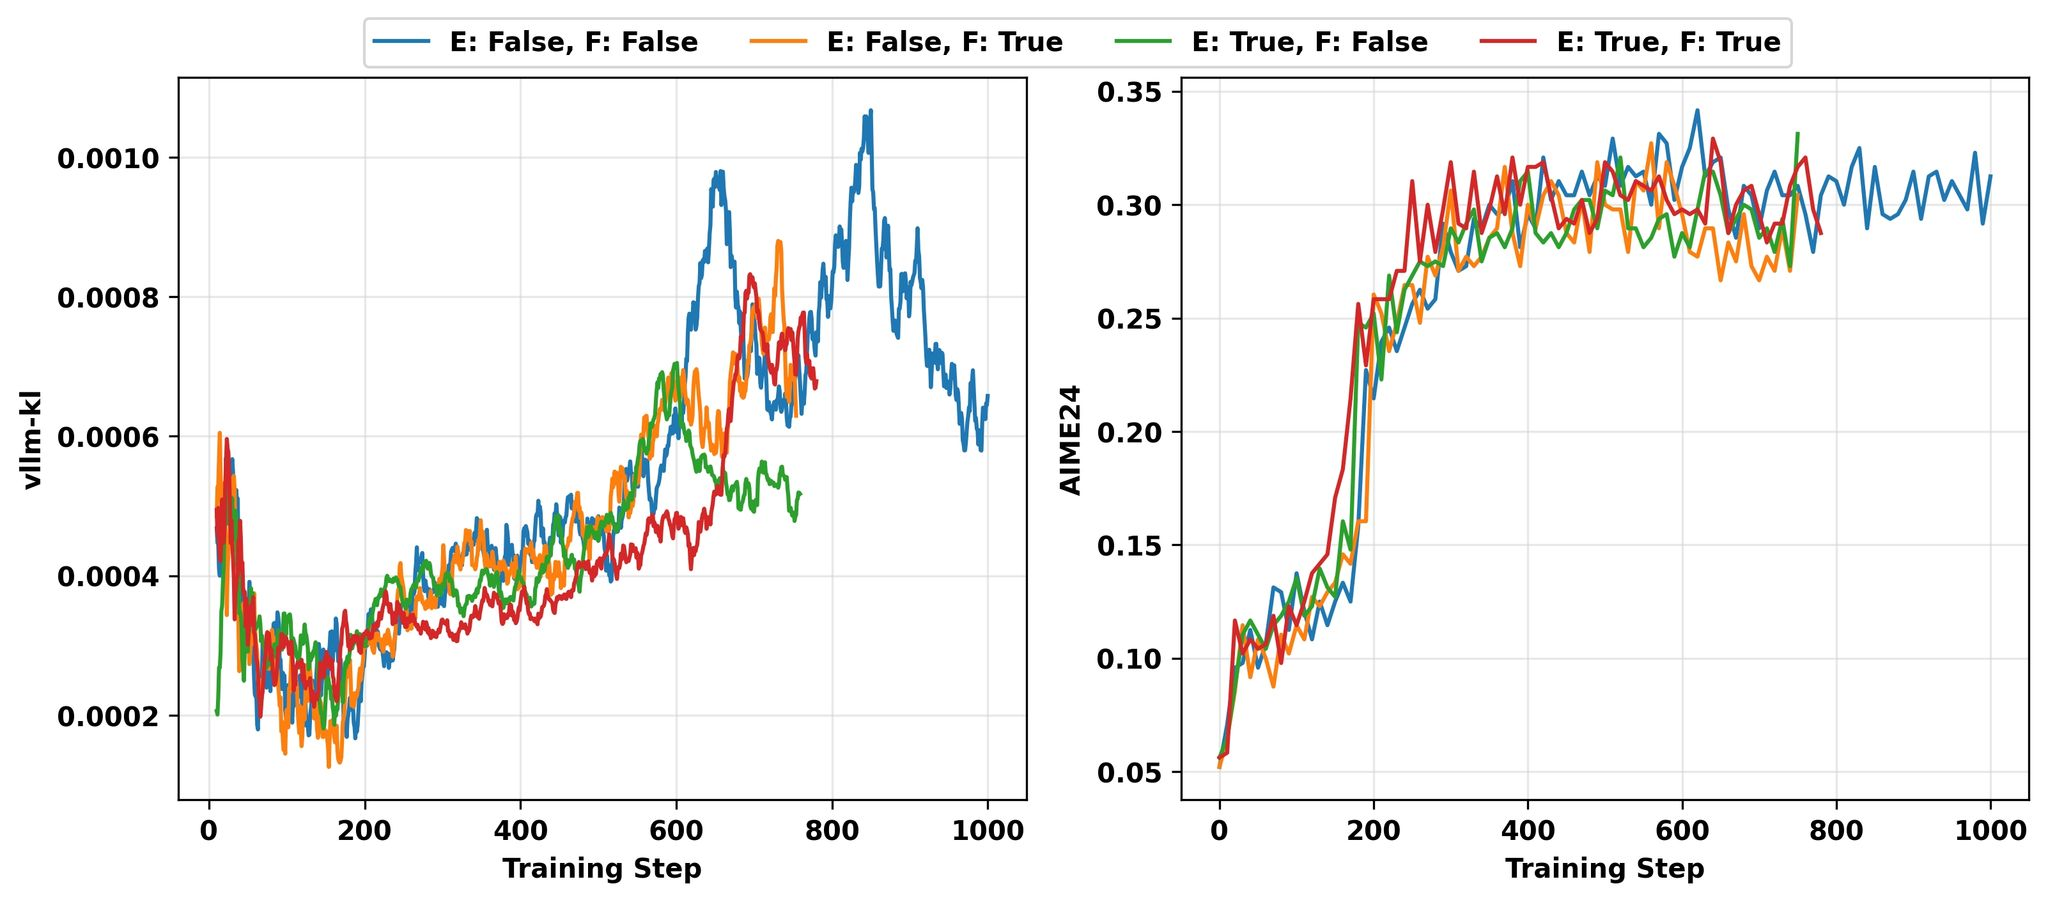
\includegraphics[width=\linewidth,height=0.64\textheight,keepaspectratio]{figures/image-19.jpg}
\caption*{\textbf{图 13。}推理强化学习中，vLLM 加速与缓存相关超参数的消融实验。在 H100 上运行同策略 GRPO，穷举 \code{enforce_eager}（E）与 \code{free_cache_engine}（F）的四种组合。左：\code{vllm-kl}；右：AIME24 准确率。}
\end{figure}


% source-block: 277211a5-58b7-8090-b5aa-dfaba7160a2c (divider; source-index: 150)

% source-block: 271211a5-58b7-801e-bd8e-d67fd96e9ee5 (sub_header; source-index: 151)

\hypertarget{src-271211a5-58b7-801e-bd8e-d67fd96e9ee5}{}
\subsection*{4.2 有效的尝试}
\phantomsection
\addcontentsline{toc}{subsection}{4.2 有效的尝试}


% source-block: 27b211a5-58b7-8099-ba48-fa8849ab54c8 (sub_sub_header; source-index: 152)

\hypertarget{src-27b211a5-58b7-8099-ba48-fa8849ab54c8}{}
\subsubsection*{4.2.1 有理论依据的方案：分布修正}


% source-block: 27b211a5-58b7-8028-a894-f39591942a0a (text; source-index: 153)

训练与推理不匹配将原本的同策略强化学习变成了异策略问题：生成 rollout 的行为策略 $\piv$ 与被训练的目标策略 $\pif$ 不同。修正这种分布偏移的一种有理论依据的方法是\textbf{重要性采样（importance sampling，IS）}。然而，重要性采样的具体形式至关重要，它决定了梯度能否保持无偏、训练能否稳定。


% source-block: 27b211a5-58b7-80ea-9015-dfe301d70459 (text; source-index: 154)

受 \href{https://fengyao.notion.site/off-policy-rl}{Yao 等人（2025）}的发现启发——该工作首先指出训练与推理不匹配导致的隐式异策略问题——我们分析两种主要形式：理论上成立的序列级重要性采样，以及常见但有偏的词元级近似。


% source-block: 289211a5-58b7-8071-b0be-e76f08be4134 (divider; source-index: 155)

% source-block: 27b211a5-58b7-80b3-8c1a-f3aee1f533e7 (sub_sub_header; source-index: 156)

\hypertarget{src-27b211a5-58b7-80b3-8c1a-f3aee1f533e7}{}
\subsubsection*{有理论依据的估计器：序列级重要性采样}


% source-block: 27b211a5-58b7-806e-ac43-e57c91c63c41 (text; source-index: 157)

正确的无偏策略梯度估计器，应当对整个生成序列（轨迹）$y$ 使用一个统一的重要性比率。这样才能将行为策略下的期望正确重加权为目标策略下的期望，得到目标函数 $J(\theta)$ 的真实梯度。


% source-block: 27b211a5-58b7-8082-aa22-de1abe0b6193 (text; source-index: 158)

下面逐步推导序列级重要性采样估计器 $g_{\mathrm{seq}}(\theta)$。


% source-block: 27b211a5-58b7-8046-af3c-d89a7eab1c3b (numbered_list; source-index: 159)

\begin{enumerate}

\item 目标是最大化目标 FSDP 策略下的期望奖励：

% source-block: 27b211a5-58b7-80d8-939a-e993347e1e33 (equation; source-index: 160)


\[
\adjustbox{max width=0.98\linewidth}{$\displaystyle J(\theta) = \mathbb{E}_{x \sim \mathcal{D}, y \sim \textcolor{blue}{\pi_{\theta}^{\mathrm{fsdp}}}(\cdot|x)}[R(x,y)]$}
\]


% source-block: 27b211a5-58b7-80d1-b104-c1de2852404a (numbered_list; source-index: 161)

\item 因此，真实策略梯度为：

% source-block: 27b211a5-58b7-80dc-8ccc-e9b652de2714 (equation; source-index: 162)


\[
\adjustbox{max width=0.98\linewidth}{$\displaystyle g(\theta) = \nabla_{\theta} J(\theta) = \mathbb{E}_{x \sim \mathcal{D}, y \sim \textcolor{blue}{\pi_{\theta}^{\mathrm{fsdp}}}(\cdot|x)}\left[R(x,y) \nabla_{\theta} \log \textcolor{blue}{\pi_{\theta}^{\mathrm{fsdp}}}(y|x)\right]$}
\]


% source-block: 27b211a5-58b7-805f-91d8-e23264b3b3e9 (numbered_list; source-index: 163)

\item 由于只能从 vLLM 策略采样，我们利用重要性采样改变期望所依据的分布：

% source-block: 27b211a5-58b7-8067-a347-c5e8224e4b20 (equation; source-index: 164)


\[
\adjustbox{max width=0.98\linewidth}{$\displaystyle g_{\mathrm{seq}}(\theta) = \mathbb{E}_{x \sim \mathcal{D}, y \sim \textcolor{red}{\pi_{\theta}^{\mathrm{vllm}}}(\cdot|x)}\left[ \frac{\textcolor{blue}{\pi_{\theta}^{\mathrm{fsdp}}}(y|x)}{\textcolor{red}{\pi_{\theta}^{\mathrm{vllm}}}(y|x)} \cdot R(x,y) \cdot \nabla_{\theta} \log \textcolor{blue}{\pi_{\theta}^{\mathrm{fsdp}}}(y|x) \right]$}
\]


\end{enumerate}

% source-block: 289211a5-58b7-8009-91d5-e73cbd4f8d0c (text; source-index: 165)

这本质上就是异策略 \href{https://doi.org/10.1007/BF00992696}{REINFORCE 算法（Williams，1992）}。该估计器与策略梯度的标准优势形式在数学上等价。关键在于证明：重要性采样比率恰好修正了期望，显露出其对应的真实同策略梯度，随后便可进一步变形。


% source-block: 289211a5-58b7-80f2-8cad-efc62fc53011 (toggle; source-index: 166)

\hypertarget{src-289211a5-58b7-80f2-8cad-efc62fc53011}{}
\paragraph*{详细推导（展开原文折叠内容）}


% source-block: 289211a5-58b7-80f7-8aed-cdffcac5b087 (sub_sub_header; source-index: 167)

\hypertarget{src-289211a5-58b7-80f7-8aed-cdffcac5b087}{}
\paragraph*{步骤 1：将期望转为同策略形式}


% source-block: 289211a5-58b7-8091-9feb-d9240d8bc783 (text; source-index: 168)

重要性采样估计器对行为策略 $\piv$ 取期望。将期望按积分展开后，行为策略密度 $p_\theta^{\mathrm{vllm}}(y\mid x)$ 可以约掉：


% source-block: 289211a5-58b7-8024-ad84-e96456fbba81 (equation; source-index: 169)


\[
\adjustbox{max width=0.98\linewidth}{$\displaystyle g_{\mathrm{seq}}(\theta) = \int \left( \frac{\pi_{\textcolor{blue}{\theta}}^{\mathrm{fsdp}}(y|x)}{\pi_{\textcolor{red}{\theta}}^{\mathrm{vllm}}(y|x)} \cdot R(x,y) \cdot \nabla_{\theta} \log \pi_{\textcolor{blue}{\theta}}^{\mathrm{fsdp}}(y|x) \right) \pi_{\textcolor{red}{\theta}}^{\mathrm{vllm}}(y|x) \,dy$}
\]

\vspace{-1em}

\[
\adjustbox{max width=0.98\linewidth}{$\displaystyle {}= \int \left( R(x,y) \cdot \nabla_{\theta} \log \pi_{\textcolor{blue}{\theta}}^{\mathrm{fsdp}}(y|x) \right) \pi_{\textcolor{blue}{\theta}}^{\mathrm{fsdp}}(y|x) \,dy$}
\]


% source-block: 289211a5-58b7-809f-a5cb-d1344b242f26 (divider; source-index: 170)

% source-block: 289211a5-58b7-808a-a07b-d1824f44cd90 (text; source-index: 171)

余下的正是真实同策略梯度，此时期望是在目标策略 $\pif$ 下计算的。这证明 $g_{\mathrm{seq}}(\theta)$ 是真实策略梯度的无偏估计器。


% source-block: 289211a5-58b7-80a7-b47e-e39882ddae36 (equation; source-index: 172)


\[
\adjustbox{max width=0.98\linewidth}{$\displaystyle g(\theta) = \mathbb{E}_{y \sim \textcolor{blue}{\pi_{\theta}^{\mathrm{fsdp}}}} \left[ R(x,y) \cdot \nabla_{\theta} \log \pi_{\textcolor{blue}{\theta}}^{\mathrm{fsdp}}(y|x) \right]$}
\]


% source-block: 289211a5-58b7-806e-b680-dfa3d1f98fe9 (sub_sub_header; source-index: 173)

\hypertarget{src-289211a5-58b7-806e-b680-dfa3d1f98fe9}{}
\paragraph*{步骤 2：按时间步分解，并应用因果性}


% source-block: 289211a5-58b7-8006-a9ea-e1305b781ddc (text; source-index: 174)

现在从更简单的同策略表达式出发，展开轨迹级各项，并应用因果性原则：第 $t$ 步动作只影响未来奖励。因此，可以把总奖励 $R(x,y)$ 替换为从当前时刻起的回报（return-to-go），$G_t=\sum_{k=t}^{|y|-1}r(s_k,a_k)$。


% source-block: 289211a5-58b7-8017-b641-f147bb98a16c (equation; source-index: 175)


\[
\adjustbox{max width=0.98\linewidth}{$\displaystyle g(\theta) = \mathbb{E}_{y \sim \textcolor{blue}{\pi_{\theta}}} \left[ \sum_{t=0}^{|y|-1} G_t \cdot \nabla_{\theta} \log \textcolor{blue}{\pi_{\theta}}(a_t|s_t) \right]$}
\]


% source-block: 289211a5-58b7-807d-936b-d5b02abe23ff (divider; source-index: 176)

% source-block: 289211a5-58b7-8086-ad70-da0fb252b068 (sub_sub_header; source-index: 177)

\hypertarget{src-289211a5-58b7-8086-ad70-da0fb252b068}{}
\paragraph*{步骤 3：引入优势函数}


% source-block: 289211a5-58b7-8004-b085-f353e303dfc3 (text; source-index: 178)

为减小方差，我们减去依赖状态的基线，即价值函数 $V^{\pi_\theta}(s_t)$。这样，未来回报就转化为优势项 $A^{\pi_\theta}(s_t,a_t)=G_t-V^{\pi_\theta}(s_t)$。\footnote{译注：原文用 $G_t-V^\pi(s_t)$ 表示优势。严格说，该量是优势的蒙特卡洛样本估计；其在给定 $(s_t,a_t)$ 下的条件期望才是 $A^\pi(s_t,a_t)=Q^\pi(s_t,a_t)-V^\pi(s_t)$。}


% source-block: 289211a5-58b7-80e2-ad00-fe5c60549689 (equation; source-index: 179)


\[
\adjustbox{max width=0.98\linewidth}{$\displaystyle g(\theta) = \mathbb{E}_{y \sim \textcolor{blue}{\pi_{\theta}}} \left[ \sum_{t=0}^{|y|-1} A^{\textcolor{blue}{\pi_{\theta}}}(s_t, a_t) \cdot \nabla_{\theta} \log \textcolor{blue}{\pi_{\theta}}(a_t|s_t) \right]$}
\]


% source-block: 289211a5-58b7-80c4-8184-f234adb21fe2 (divider; source-index: 180)

% source-block: 289211a5-58b7-8039-aa9c-faafbb089f1e (sub_sub_header; source-index: 181)

\hypertarget{src-289211a5-58b7-8039-aa9c-faafbb089f1e}{}
\paragraph*{步骤 4：转为状态级期望}


% source-block: 289211a5-58b7-805f-8306-fbcf3f39a585 (text; source-index: 182)

最后，将轨迹上的期望改写为目标策略诱导的状态访问测度 $d_{\pi_\theta}$ 上的等价形式。


% source-block: 289211a5-58b7-801b-8cb8-c5121dea3004 (toggle; source-index: 183)

\hypertarget{src-289211a5-58b7-801b-8cb8-c5121dea3004}{}
\paragraph*{从步骤 3 到步骤 4 的详细数学过程（展开原文折叠内容）}


% source-block: 289211a5-58b7-8091-8e88-d1459cd4b521 (sub_sub_header; source-index: 184)

\hypertarget{src-289211a5-58b7-8091-8e88-d1459cd4b521}{}
\paragraph*{步骤 A：从轨迹级期望出发}


% source-block: 289211a5-58b7-80f3-b219-ef5813cd4226 (equation; source-index: 185)


\[
\adjustbox{max width=0.98\linewidth}{$\displaystyle g(\theta) = \mathbb{E}_{y \sim \textcolor{blue}{\pi_{\theta}}} \left[ \sum_{t=0}^{|y|-1} A^{\textcolor{blue}{\pi_{\theta}}}(s_t, a_t) \cdot \nabla_{\theta} \log \textcolor{blue}{\pi_{\theta}}(a_t|s_t) \right]$}
\]


% source-block: 289211a5-58b7-80dd-9b6a-e71ce6012607 (sub_sub_header; source-index: 186)

\hypertarget{src-289211a5-58b7-80dd-9b6a-e71ce6012607}{}
\paragraph*{步骤 B：应用期望的线性性质}


% source-block: 289211a5-58b7-8076-af07-c38a885217b1 (text; source-index: 187)

交换期望与求和。轨迹长度 $|y|$ 有限，超过该长度的时间步对应项均为零，因此可以将求和上限扩展至无穷，这只是补上若干零项。


% source-block: 289211a5-58b7-80e4-8ae8-cdc592bf318b (equation; source-index: 188)


\[
\adjustbox{max width=0.98\linewidth}{$\displaystyle g(\theta) = \sum_{t=0}^{\infty} \mathbb{E}_{y \sim \textcolor{blue}{\pi_{\theta}}} \left[ A^{\textcolor{blue}{\pi_{\theta}}}(s_t, a_t) \cdot \nabla_{\theta} \log \textcolor{blue}{\pi_{\theta}}(a_t|s_t) \right]$}
\]


% source-block: 289211a5-58b7-8070-ba4c-ea6524d1ccaa (sub_sub_header; source-index: 189)

\hypertarget{src-289211a5-58b7-8070-ba4c-ea6524d1ccaa}{}
\paragraph*{步骤 C：将期望展开为显式求和}


% source-block: 289211a5-58b7-8021-a3a8-c6030a5f4ac6 (text; source-index: 190)

对所有可能状态 $s$ 和动作 $a$ 求和，以联合概率 $P(s_t=s,a_t=a)=P(s_t=s)\cdot\pi_\theta(a\mid s)$ 加权，从而改写内部期望。


% source-block: 289211a5-58b7-8087-9363-d6ae518b6599 (equation; source-index: 191)


\[
\adjustbox{max width=0.98\linewidth}{$\displaystyle g(\theta) = \sum_{t=0}^{\infty} \sum_{s \in \mathcal{S}} P(s_t=s | \textcolor{blue}{\pi_{\theta}}) \sum_{a \in \mathcal{A}} \textcolor{blue}{\pi_{\theta}}(a|s) \cdot \left[ A^{\textcolor{blue}{\pi_{\theta}}}(s, a) \cdot \nabla_{\theta} \log \textcolor{blue}{\pi_{\theta}}(a|s) \right]$}
\]


% source-block: 289211a5-58b7-80d3-89b0-e29d8e957a4f (sub_sub_header; source-index: 192)

\hypertarget{src-289211a5-58b7-80d3-89b0-e29d8e957a4f}{}
\paragraph*{步骤 D：引入状态占用测度}


% source-block: 289211a5-58b7-80bf-8967-f3ac6f31819b (text; source-index: 193)

重排求和，将与状态 $s$ 有关的项归并在一起。


% source-block: 289211a5-58b7-8025-8d2b-fa528388c13c (equation; source-index: 194)


\[
\adjustbox{max width=0.98\linewidth}{$\displaystyle g(\theta) = \sum_{s \in \mathcal{S}} \left( \sum_{t=0}^{\infty} P(s_t=s | \textcolor{blue}{\pi_{\theta}}) \right) \left( \sum_{a \in \mathcal{A}} \textcolor{blue}{\pi_{\theta}}(a|s) \cdot \left[ \dots \right] \right)$}
\]


% source-block: 289211a5-58b7-80fc-af18-e31010bab8fa (text; source-index: 195)

第一项 $\sum_{t=0}^{\infty}P(s_t=s)$ 定义了状态占用测度 $d_{\pi_\theta}(s)$；第二项则是动作上的期望 $\mathbb E_{a\sim\pi_\theta(\cdot\mid s)}[\dots]$。


% source-block: 289211a5-58b7-809e-84e4-f908f366ea96 (equation; source-index: 196)


\[
\adjustbox{max width=0.98\linewidth}{$\displaystyle g(\theta) = \sum_{s \in \mathcal{S}} d_{\textcolor{blue}{\pi_{\theta}}}(s) \cdot \mathbb{E}_{a \sim \textcolor{blue}{\pi_{\theta}}(\cdot|s)} \left[ A^{\textcolor{blue}{\pi_{\theta}}}(s, a) \cdot \nabla_{\theta} \log \textcolor{blue}{\pi_{\theta}}(a|s) \right]$}
\]


% source-block: 289211a5-58b7-80f8-bec6-ccdcdd2dd674 (sub_sub_header; source-index: 197)

\hypertarget{src-289211a5-58b7-80f8-bec6-ccdcdd2dd674}{}
\paragraph*{步骤 E：得到最终形式}


% source-block: 289211a5-58b7-80ea-9606-c93b801e00ea (text; source-index: 198)

按照原文的记号，对状态占用测度加权求和，写作在 $d_{\pi_\theta}$ 上取“期望”。\footnote{译注：原文定义 $d_\pi(s)=\sum_tP(s_t=s\mid\pi)$，它是未归一化的占用测度，总质量为期望轨迹长度。文中的 $\mathbb E_{s\sim d_\pi}$ 应按对该测度积分理解；若将 $d_\pi$ 归一化为概率分布，则需保留相应的总质量因子。}


% source-block: 289211a5-58b7-8075-a61a-ee89489e5bca (equation; source-index: 199)


\[
\adjustbox{max width=0.98\linewidth}{$\displaystyle g(\theta) = \mathbb{E}_{s \sim d_{\textcolor{blue}{\pi_{\theta}}}} \left[ \mathbb{E}_{a \sim \textcolor{blue}{\pi_{\theta}}(\cdot|s)} \left[ A^{\textcolor{blue}{\pi_{\theta}}}(s,a) \cdot \nabla_{\theta} \log \textcolor{blue}{\pi_{\theta}}(a|s) \right] \right]$}
\]


% source-block: 289211a5-58b7-808a-b58a-eca7e54243df (text; source-index: 200)

% source-block: 289211a5-58b7-8060-a9be-da7f35d08b75 (text; source-index: 201)

经过这些推导，得到策略梯度的最终优势形式：


% source-block: 289211a5-58b7-80b4-bcdb-da10cf597072 (equation; source-index: 202)


\[
\adjustbox{max width=0.98\linewidth}{$\displaystyle g_{\mathrm{seq}}(\theta) = \mathbb{E}_{s \sim d_{\textcolor{blue}{\pi_{\theta}^{\mathrm{fsdp}}}}} \mathbb{E}_{a \sim \textcolor{blue}{\pi_{\theta}^{\mathrm{fsdp}}}(\cdot|s)} \left[ A^{\textcolor{blue}{\pi_{\theta}^{\mathrm{fsdp}}}}(s,a) \cdot \nabla_{\theta} \log \textcolor{blue}{\pi_{\theta}^{\mathrm{fsdp}}}(a|s) \right]$}
\]


% source-block: 27b211a5-58b7-8039-a35a-d71630e066ff (text; source-index: 203)

这里，$s=(x,y_{<t})$ 是状态（前缀），$a=y_t$ 是动作（词元）。$d_{\pif}$ 是目标 FSDP 策略下的状态占用测度，其正式定义为：遵循策略 $\pi$ 时，状态 $s$ 被访问次数的期望。


% source-block: 27b211a5-58b7-80bf-99b1-cdf1930a09eb (equation; source-index: 204)


\[
\adjustbox{max width=0.98\linewidth}{$\displaystyle \textcolor{blue}{d_{\pi}(s) := \mathbb{E}_{x' \sim \mathcal{D}, y' \sim \pi(\cdot|x')} \left[ \sum_{t'=0}^{|y'|-1} \mathbb{I}\{ (x', y'_{<t'}) = s \} \right] = P(x) \cdot \prod_{k=0}^{t-1} \pi(y_k|x,y_{<k})}$}
\]


% source-block: 27b211a5-58b7-8086-a833-dbc5963166e0 (text; source-index: 205)

该估计器无偏，即 $g_{\mathrm{seq}}(\theta)=g(\theta)$。为提高数值稳定性，实际使用\textbf{截断重要性采样（truncated importance sampling，TIS）}，将序列级比率 $\rho(y\mid x)$ 在常数 $C$ 处截断。\footnote{译注：无偏结论针对未截断的重要性采样，并要求行为策略覆盖目标策略的支持集等常规条件。截断后的 TIS，以及下文掩码后的 MIS，一般都会引入偏差；原文此处保留的是对未截断估计器的无偏性陈述。}


% source-block: 27b211a5-58b7-80ea-a3f0-f3ea70b3986a (divider; source-index: 206)

% source-block: 27b211a5-58b7-80a6-9cb7-c2c0f2290efa (sub_sub_header; source-index: 207)

\hypertarget{src-27b211a5-58b7-80a6-9cb7-c2c0f2290efa}{}
\subsubsection*{常见的有偏估计器：词元级重要性采样}


% source-block: 27b211a5-58b7-804d-b908-ec1b23283224 (text; source-index: 208)

一种常见启发式方法受 PPO 等算法启发，在每个词元上施加重要性比率；\href{https://fengyao.notion.site/off-policy-rl}{Yao 等人（2025）}也采用了这种方法。虽然它通常比序列级比率的方差更低，但它是一个有偏估计器。作者认为，将其作为自回归模型的精确梯度修正，在理论上并不成立。


% source-block: 27b211a5-58b7-80cd-8895-d6444106476d (text; source-index: 209)

下面推导词元级重要性采样梯度估计器 $g_{\mathrm{tok}}(\theta)$。


% source-block: 27b211a5-58b7-80b8-80c4-cd9678148d55 (numbered_list; source-index: 210)

\begin{enumerate}

\item 该形式从把重要性采样比率放入时间步求和内部开始；作者指出，若要得到精确修正，这样处理并不正确。也就是说，$g_{\mathrm{tok}}(\theta)$ 被定义为：

% source-block: 27b211a5-58b7-80c8-913e-cbaecbb9ea8e (equation; source-index: 211)


\[
\adjustbox{max width=0.98\linewidth}{$\displaystyle \mathbb{E}_{x \sim \mathcal{D}, y \sim \textcolor{red}{\pi_{\theta}^{\mathrm{vllm}}}(\cdot|x)}\left[ R(x,y) \cdot \sum_{t=0}^{|y|-1} \frac{\textcolor{blue}{\pi_{\theta}^{\mathrm{fsdp}}}(y_t|x,y_{<t})}{\textcolor{red}{\pi_{\theta}^{\mathrm{vllm}}}(y_t|x,y_{<t})} \cdot \nabla_{\theta} \log \textcolor{blue}{\pi_{\theta}^{\mathrm{fsdp}}}(y_t|x,y_{<t}) \right]$}
\]


% source-block: 27b211a5-58b7-8092-a371-e66d97325fb6 (numbered_list; source-index: 212)

\item 可以将轨迹上的期望，改写为 vLLM 策略所访问状态上的期望：

% source-block: 27b211a5-58b7-80c6-aed3-d2e7a39e4c99 (equation; source-index: 213)


\[
\adjustbox{max width=0.98\linewidth}{$\displaystyle g_{\mathrm{tok}}(\theta) = \mathbb{E}_{s \sim d_{\textcolor{red}{\pi_{\theta}^{\mathrm{vllm}}}}} \mathbb{E}_{a \sim \textcolor{red}{\pi_{\theta}^{\mathrm{vllm}}}(\cdot|s)} \left[ \frac{\textcolor{blue}{\pi_{\theta}^{\mathrm{fsdp}}}(a|s)}{\textcolor{red}{\pi_{\theta}^{\mathrm{vllm}}}(a|s)} \cdot A^{\textcolor{red}{\pi_{\theta}^{\mathrm{vllm}}}}(s,a) \cdot \nabla_{\theta} \log \textcolor{blue}{\pi_{\theta}^{\mathrm{fsdp}}}(a|s) \right]$}
\]


% source-block: 27b211a5-58b7-80b5-bbcd-eb308ea91cba (numbered_list; source-index: 214)

\item \textit{注意：这里的 $R(x,y)$ 是由 $\piv$ 采样完整轨迹得到的经验回报，充当状态动作价值 $Q^{\piv}(s,a)$ 的蒙特卡洛估计。}引入基线并改变动作期望所依据的分布，得到最终形式：

% source-block: 27b211a5-58b7-804e-b8cf-e67c868eb617 (equation; source-index: 215)


\[
\adjustbox{max width=0.98\linewidth}{$\displaystyle g_{\mathrm{tok}}(\theta) = \mathbb{E}_{s \sim d_{\textcolor{red}{\pi_{\theta}^{\mathrm{vllm}}}}} \mathbb{E}_{a \sim \textcolor{blue}{\pi_{\theta}^{\mathrm{fsdp}}}(\cdot|s)} \left[ A^{\textcolor{red}{\pi_{\theta}^{\mathrm{vllm}}}}(s,a) \cdot \nabla_{\theta} \log \textcolor{blue}{\pi_{\theta}^{\mathrm{fsdp}}}(a|s) \right]$}
\]


\end{enumerate}

% source-block: 2bd211a5-58b7-8072-a024-ffc02a8003bb (text; source-index: 216)

最终表达式清楚揭示了词元级重要性采样的梯度偏差。只有当 $\piv$ 保持在 $\pif$ 的信赖域内，使 $d_{\piv}\approx d_{\pif}$ 且 $A^{\piv}\approx A^{\pif}$ 时，才能利用 $g_{\mathrm{tok}}(\theta)$ 优化 $J(\theta)$。


% source-block: 2bd211a5-58b7-8050-9776-f66576f19645 (text; source-index: 217)

% source-block: 27b211a5-58b7-80e8-8fa5-f1881eebd895 (divider; source-index: 218)

% source-block: 27b211a5-58b7-807b-88a0-ed3abb1a0eea (sub_sub_header; source-index: 219)

\hypertarget{src-27b211a5-58b7-807b-88a0-ed3abb1a0eea}{}
\subsubsection*{词元级重要性采样的偏差来源}


% source-block: 27b211a5-58b7-8033-9d71-f60621840386 (text; source-index: 220)

将 $g_{\mathrm{tok}}(\theta)$ 与真实梯度 $g_{\mathrm{seq}}(\theta)$ 比较，可以发现两个不同且显著的误差来源，它们使词元级估计器产生偏差。


% source-block: 27b211a5-58b7-80fd-a20c-f07a56e3a9a9 (sub_sub_header; source-index: 221)

\hypertarget{src-27b211a5-58b7-80fd-a20c-f07a56e3a9a9}{}
\subsubsection*{来源 1：状态占用不匹配}


% source-block: 27b211a5-58b7-806a-9a0f-ed068ec37364 (text; source-index: 222)

合理的异策略修正必须同时处理两种分布偏移：动作概率的偏移，以及状态访问概率的偏移。词元级方法只修正了前者。


% source-block: 27b211a5-58b7-806a-839d-d5acc2f507c9 (bulleted_list; source-index: 223)

\begin{itemize}

\item \textbf{真实梯度（$g_{\mathrm{seq}}$）：}对正确的目标 FSDP 分布下访问的状态取期望，即 $\mathbb E_{s\sim d_{\pif}}$。

% source-block: 27b211a5-58b7-8059-bc47-d7971240e2a0 (bulleted_list; source-index: 224)

\item \textbf{有缺陷的梯度（$g_{\mathrm{tok}}$）：}仍对行为 vLLM 分布下访问的状态取期望，即 $\mathbb E_{s\sim d_{\piv}}$。

\end{itemize}

% source-block: 27b211a5-58b7-809f-8db5-d3c658a36d34 (text; source-index: 225)

这相当于隐含假设状态占用比率为 1，即 $d_{\pi^{\mathrm{fsdp}}}(s)/d_{\pi^{\mathrm{vllm}}}(s)=1$。在自回归模型中，这一假设可能被严重违反：由于状态转移是确定性的，只要某个词元的选择不同，后续前缀状态轨迹就会完全分叉。忽略这一点，会使 $g_{\mathrm{tok}}(\theta)$ 引入很大且不受控制的偏差。


% source-block: 27b211a5-58b7-802b-83de-e69ca2d3187e (sub_sub_header; source-index: 226)

\hypertarget{src-27b211a5-58b7-802b-83de-e69ca2d3187e}{}
\subsubsection*{来源 2：奖励信号不匹配}


% source-block: 27b211a5-58b7-8041-9fcd-da1271e86d50 (text; source-index: 227)

第二个关键误差是：词元级梯度使用了另一种策略的奖励信号来加权更新。


% source-block: 27b211a5-58b7-80f4-9abe-d8309854198b (bulleted_list; source-index: 228)

\begin{itemize}

\item \textbf{真实梯度（$g_{\mathrm{seq}}$）：}更新由目标 FSDP 策略的优势函数 $A^{\pif}$ 缩放，它表示该策略下的预期未来奖励。

% source-block: 27b211a5-58b7-8034-89d9-d463f69f8565 (bulleted_list; source-index: 229)

\item \textbf{有缺陷的梯度（$g_{\mathrm{tok}}$）：}更新由行为 vLLM 策略的优势函数 $A^{\piv}$ 缩放。

\end{itemize}

% source-block: 27b211a5-58b7-8019-bbfe-e109de1671a2 (text; source-index: 230)

目标策略的梯度被属于行为策略的奖励信号缩放。状态分布与奖励信号都存在根本性不匹配，因此词元级梯度有偏，不能作为理论上精确的估计器。


% source-block: 27b211a5-58b7-8047-8961-ca6df2c07d96 (callout; source-index: 231)

% source-block: 27b211a5-58b7-8078-911a-f1aea4303053 (text; source-index: 232)

上述理论表明，尽管词元级方法可能具有更低方差，梯度偏差仍然存在，并可能导致训练不稳定；后续实验也证实了这一预测。关于词元级与序列级方法的详细偏差、方差分析，见系列博客\href{https://richardli.xyz/rl-collapse-1}{第一篇}和\href{https://richardli.xyz/rl-collapse-2}{第二篇}。


% source-block: 27b211a5-58b7-80f0-9e0e-c6e4cf2f846f (divider; source-index: 233)

% source-block: 27b211a5-58b7-8081-8192-d3f2dc686da4 (sub_sub_header; source-index: 234)

\hypertarget{src-27b211a5-58b7-8081-8192-d3f2dc686da4}{}
\subsubsection*{实验验证}


% source-block: 27b211a5-58b7-80b4-aa84-c1f173bd3842 (text; source-index: 235)

我们的理论分析预测：有偏的词元级重要性采样会不稳定并最终失败，而无偏的序列级重要性采样会更稳健。我们的实验支持这一判断。


% source-block: 27b211a5-58b7-80cc-860e-d7fb96fdf309 (sub_sub_header; source-index: 236)

\hypertarget{src-27b211a5-58b7-80cc-860e-d7fb96fdf309}{}
\subsubsection*{重要性采样避免了梯度爆炸，但词元级方法仍然失败}


% source-block: 27b211a5-58b7-8019-8075-f3f7b3a8354d (text; source-index: 237)

我们从 L20 上一个崩溃实验的第 200 步恢复训练，分别加入词元级 TIS 和序列级 TIS（$C=2$）。如图 14 所示，两种方法起初都避免了原始实验中的梯度爆炸，但词元级 TIS 实验随后仍然崩溃；序列级 TIS 实验则保持稳定。这支持了我们的理论：词元级方法的有偏梯度最终可能导致失败。


% source-block: 271211a5-58b7-8008-aab6-ca175a776bdd (image; source-index: 238)

\begin{figure}[H]
\centering
% source-block: 271211a5-58b7-8008-aab6-ca175a776bdd (image)
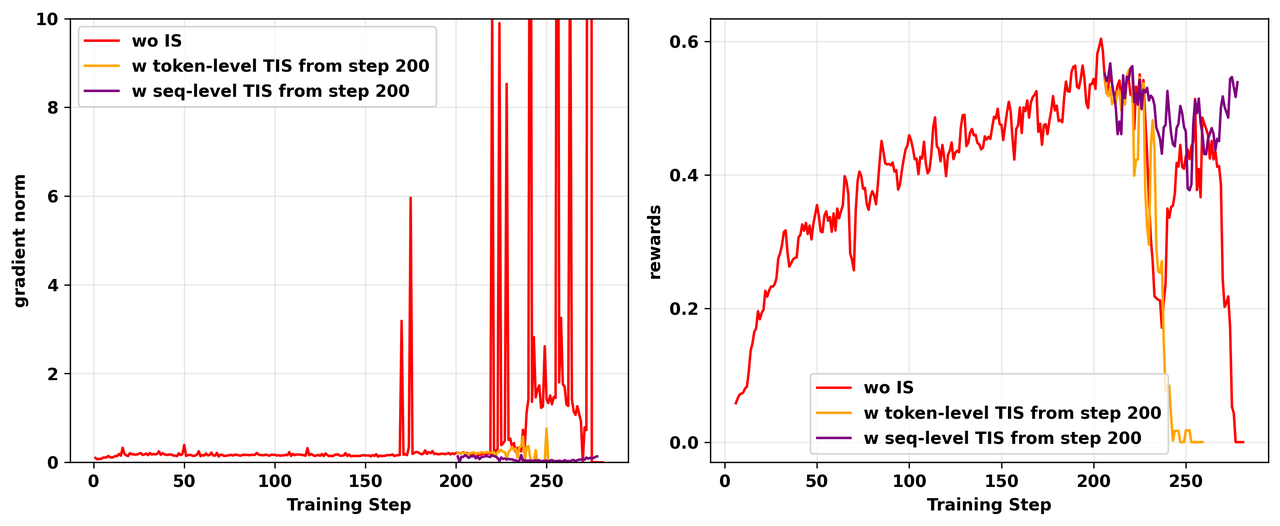
\includegraphics[width=\linewidth,height=0.64\textheight,keepaspectratio]{figures/image-20.png}
\caption*{\textbf{图 14。}不同 TIS 策略的消融实验。未使用重要性采样的原始同策略实验在 200 步后崩溃并出现梯度爆炸；另外两次实验分别从第 200 步恢复，并加入词元级 TIS 或序列级 TIS。左：梯度范数；右：训练奖励。}
\end{figure}


% source-block: 27b211a5-58b7-8016-9cb8-ff6f0de98a30 (sub_sub_header; source-index: 239)

\hypertarget{src-27b211a5-58b7-8016-9cb8-ff6f0de98a30}{}
\subsubsection*{推理强化学习中的词元级 TIS}


% source-block: 27b211a5-58b7-8039-9112-d72fa45bb16d (text; source-index: 240)

虽然词元级 TIS 在复杂 TIR 实验中失败，但对于不匹配较小的简单推理强化学习，它可以帮助防止崩溃。在同策略 GRPO 和 RLOO 实验中（图 15），词元级 TIS 避免了梯度爆炸；不过训练依然不稳定，也没有取得更好的最终性能，其潜在原因可能仍是梯度偏差。


% source-block: 271211a5-58b7-80a6-89b2-f5313ed260bf (image; source-index: 241)

\begin{figure}[H]
\centering
% source-block: 271211a5-58b7-80a6-89b2-f5313ed260bf (image)
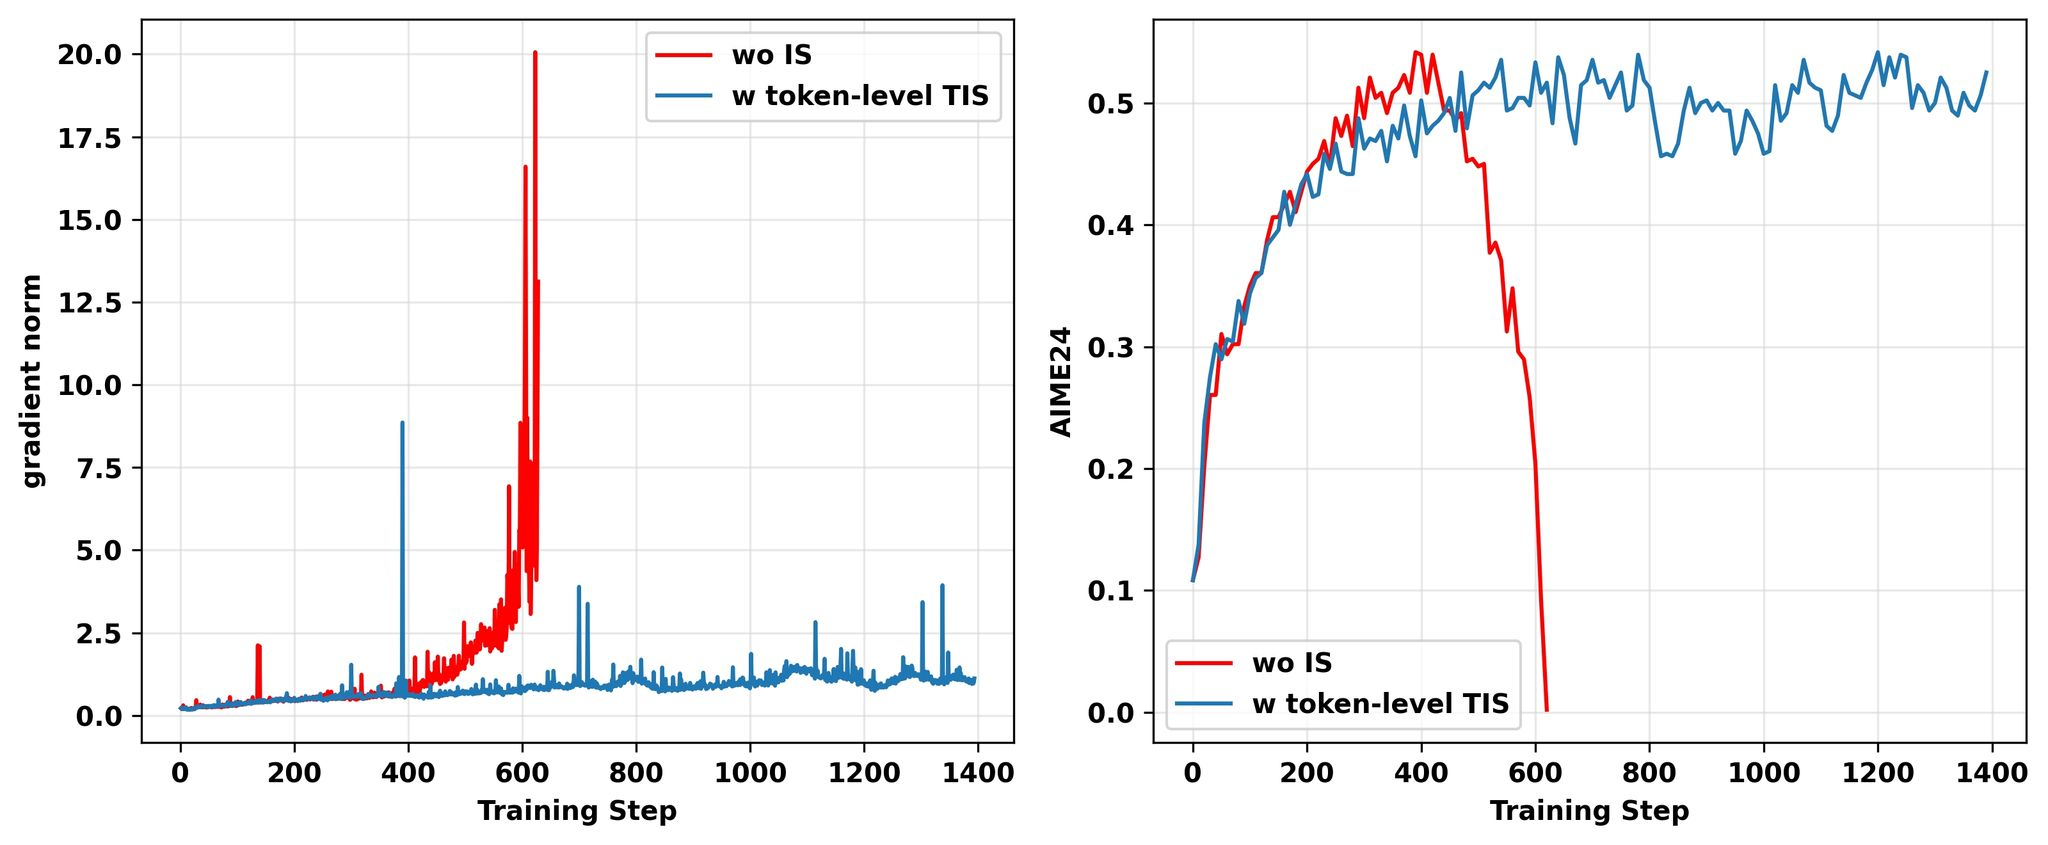
\includegraphics[width=\linewidth,height=0.64\textheight,keepaspectratio]{figures/image-21.jpg}
\caption*{\textbf{图 15(a)。}H100 上推理强化学习的同策略 GRPO 实验：不使用重要性采样，与使用词元级重要性采样（$C=2$）的比较。左：梯度范数；右：AIME24 准确率。词元级 TIS 避免了训练崩溃，但没有取得更好的测试性能。}
\end{figure}


% source-block: 27b211a5-58b7-80b6-8007-d80f67c22b85 (image; source-index: 242)

\begin{figure}[H]
\centering
% source-block: 27b211a5-58b7-80b6-8007-d80f67c22b85 (image)
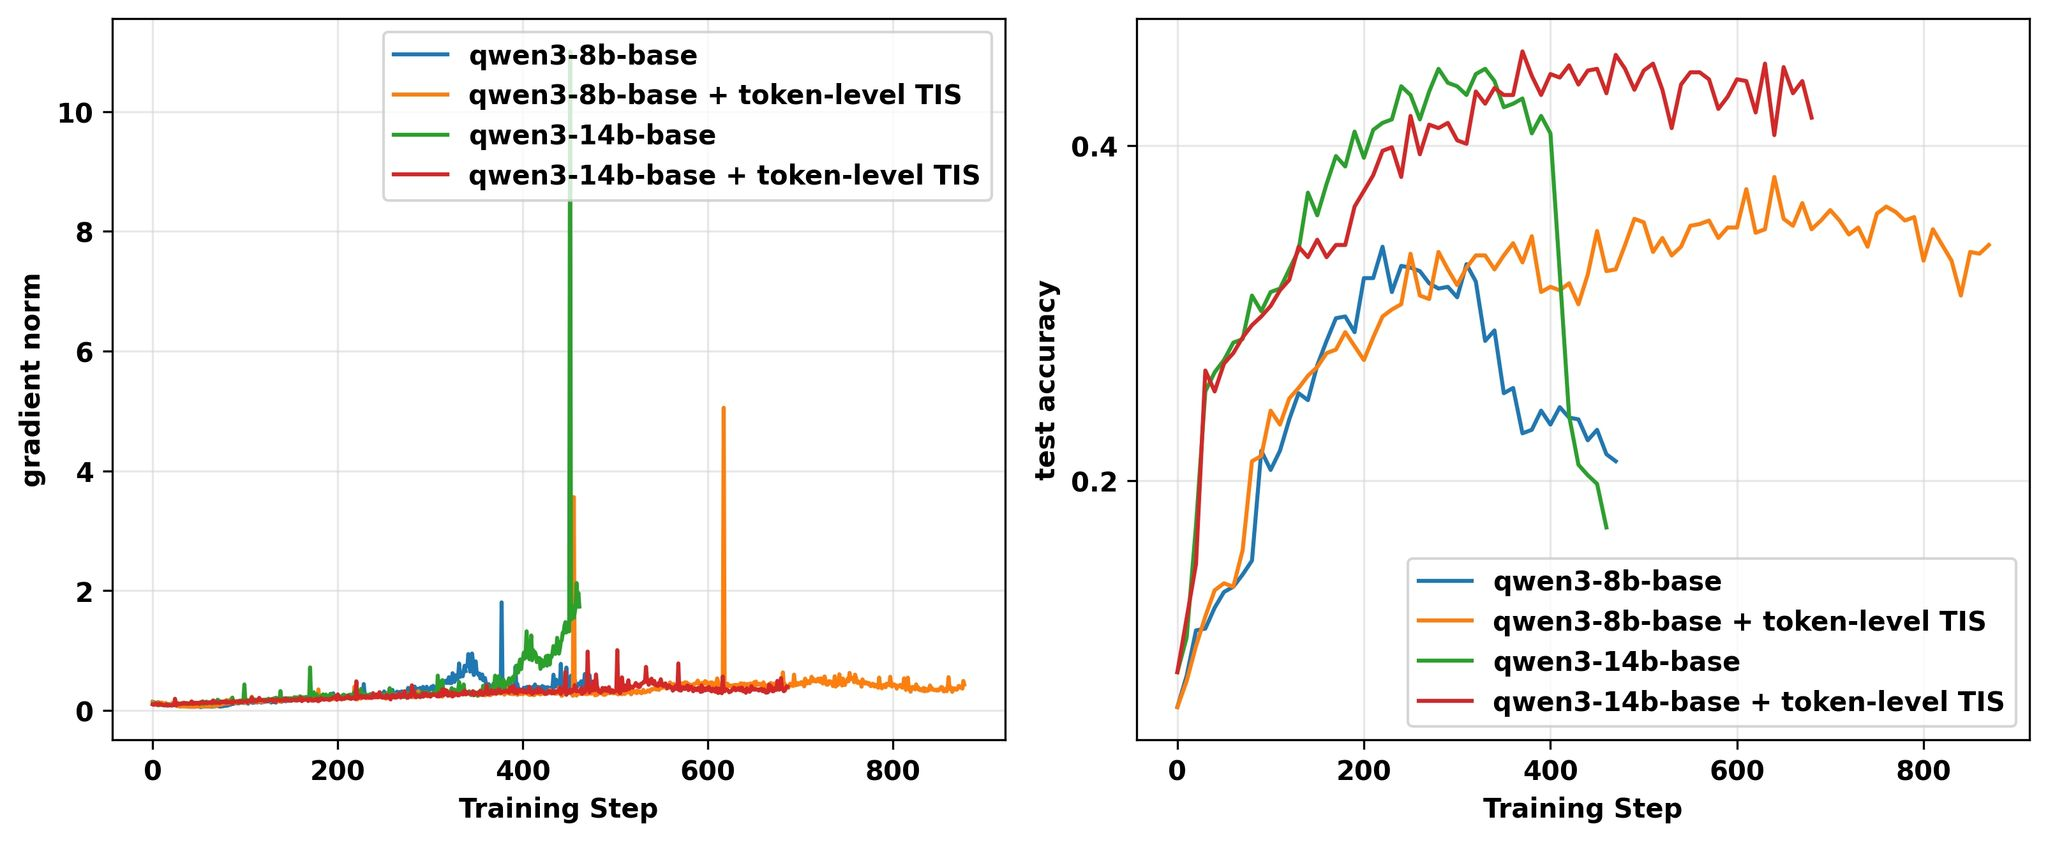
\includegraphics[width=\linewidth,height=0.64\textheight,keepaspectratio]{figures/image-22.jpg}
\caption*{\textbf{图 15(b)。}H100 上推理强化学习的同策略 RLOO 实验：不使用重要性采样，与使用词元级重要性采样（$C=2$）的比较。左：梯度范数；右：AIME24/AIME25 平均准确率。词元级 TIS 缓解了崩溃，但没有取得更好的测试性能，后期还有性能下降趋势。}
\end{figure}


% source-block: 27b211a5-58b7-809c-95f3-c38299424cb3 (sub_sub_header; source-index: 243)

\hypertarget{src-27b211a5-58b7-809c-95f3-c38299424cb3}{}
\subsubsection*{TIS 延长了训练，但仍可能不稳定}


% source-block: 27b211a5-58b7-8074-8280-d60a1f521829 (text; source-index: 244)

我们在 L20 GPU 上，从头开展使用序列级 TIS（$C=2$）的同策略 TIR 实验。如图 16 所示，虽然该方法避免了彻底崩溃，但奖励达到平台期后持续波动，测试性能也没有超过原始实验崩溃前达到的峰值。


% source-block: 27b211a5-58b7-80aa-abaf-e901a524bca8 (image; source-index: 245)

\begin{figure}[H]
\centering
% source-block: 27b211a5-58b7-80aa-abaf-e901a524bca8 (image)
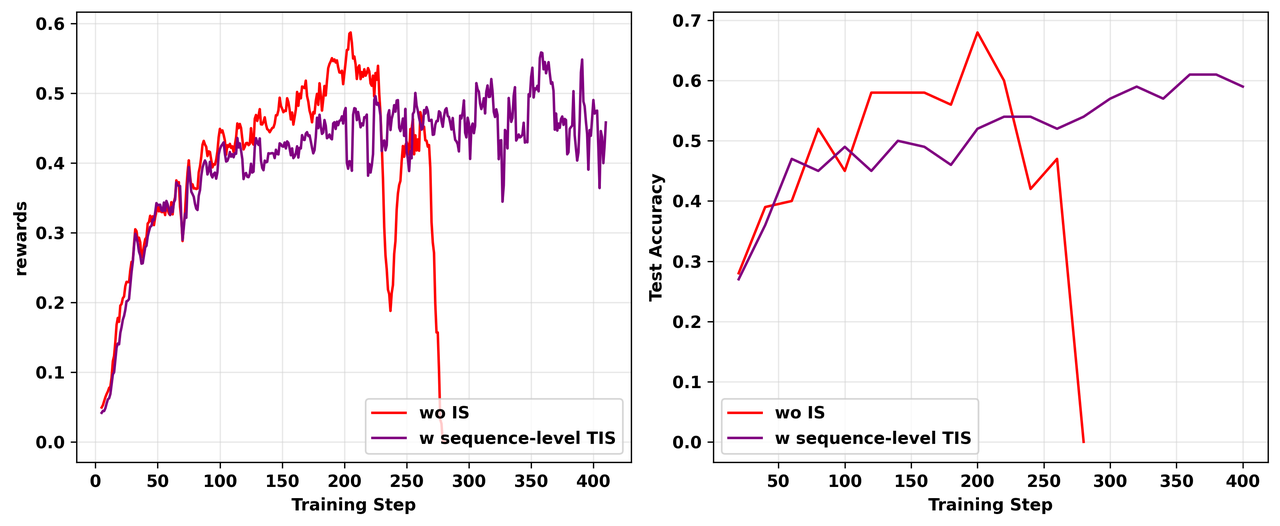
\includegraphics[width=\linewidth,height=0.64\textheight,keepaspectratio]{figures/image-23.png}
\caption*{\textbf{图 16。}不同 TIS 策略的进一步消融。未使用重要性采样的原始同策略实验在 200 步后崩溃；另一实验从头运行，配置相同，但加入 $C=2$ 的序列级 TIS。左：训练奖励；右：测试准确率。}
\end{figure}


% source-block: 27b211a5-58b7-8018-a714-c70402ddf952 (sub_sub_header; source-index: 246)

\hypertarget{src-27b211a5-58b7-8018-a714-c70402ddf952}{}
\subsubsection*{掩码重要性采样（MIS）}


% source-block: 27b211a5-58b7-80d0-a036-ddcfbe517351 (text; source-index: 247)

为改进 TIS，我们提出\textbf{掩码重要性采样（masked importance sampling，MIS）}：对重要性采样比率超过阈值 $C$ 的序列，将其策略损失掩掉，即 $\rho(y\mid x)\gets\rho(y\mid x)\mathbb I\{\rho(y\mid x)\le C\}$。图 17 表明，MIS 提高了训练稳定性，并在训练奖励和测试准确率上都超过了原始实验与 TIS 实验的峰值。\footnote{译注：原文正文强调稳定性的改善，而图 17 图注同时指出，MIS 和 TIS 在后期都仍存在不稳定性。译文保留两处表述，不能据此理解为 MIS 保证所有阶段稳定。}


% source-block: 27b211a5-58b7-808b-92f0-f53e0439f9d6 (image; source-index: 248)

\begin{figure}[H]
\centering
% source-block: 27b211a5-58b7-808b-92f0-f53e0439f9d6 (image)
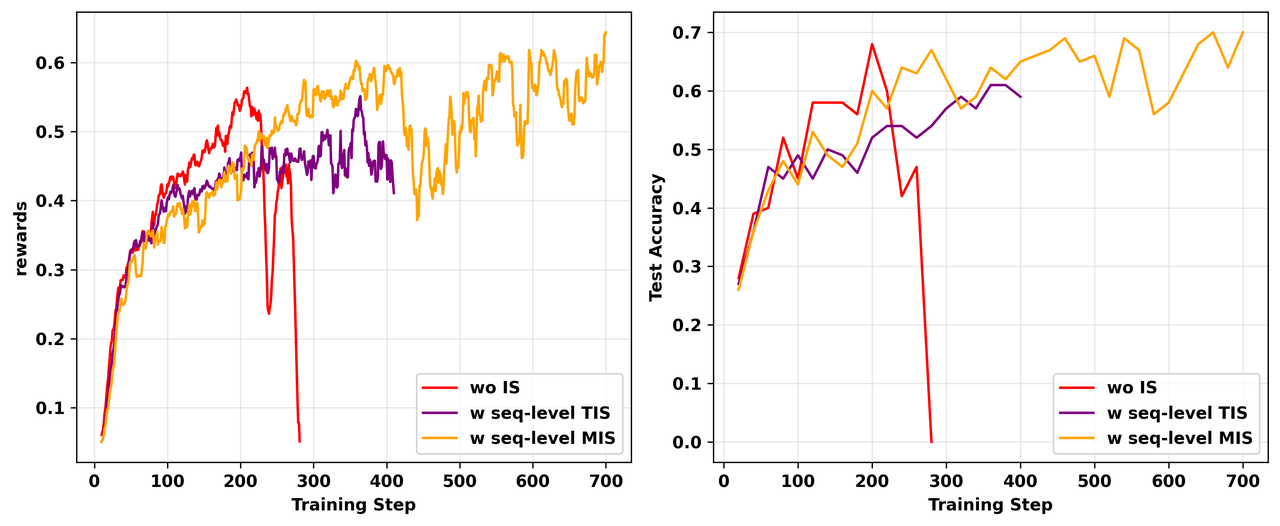
\includegraphics[width=\linewidth,height=0.64\textheight,keepaspectratio]{figures/image-24.png}
\caption*{\textbf{图 17。}L20 上同策略 GRPO 的序列级 MIS、序列级 TIS 与未使用重要性采样的原始版本对比。MIS 与 TIS 均延长了训练时间，但后期仍存在不稳定性。MIS 在训练奖励和测试准确率上均优于 TIS，并超过原始实验的峰值。左：训练奖励；右：测试准确率。}
\end{figure}


% source-block: 27b211a5-58b7-8051-a317-d40175e29b7a (sub_sub_header; source-index: 249)

\hypertarget{src-27b211a5-58b7-8051-a317-d40175e29b7a}{}
\subsubsection*{词元级 MIS 与序列级 MIS}


% source-block: 27b211a5-58b7-80c5-aac5-c904c8662cee (text; source-index: 250)

最后，我们比较了词元级和序列级 MIS。如预期，图 18 表明，虽然两者都避免了初期梯度爆炸，但词元级 MIS 实验仍然崩溃。这再次支持我们的结论：对于复杂、长时域的自回归任务，有理论依据的序列级修正更加可靠。


% source-block: 27b211a5-58b7-80a9-9837-dc6b5f980e1b (image; source-index: 251)

\begin{figure}[H]
\centering
% source-block: 27b211a5-58b7-80a9-9837-dc6b5f980e1b (image)
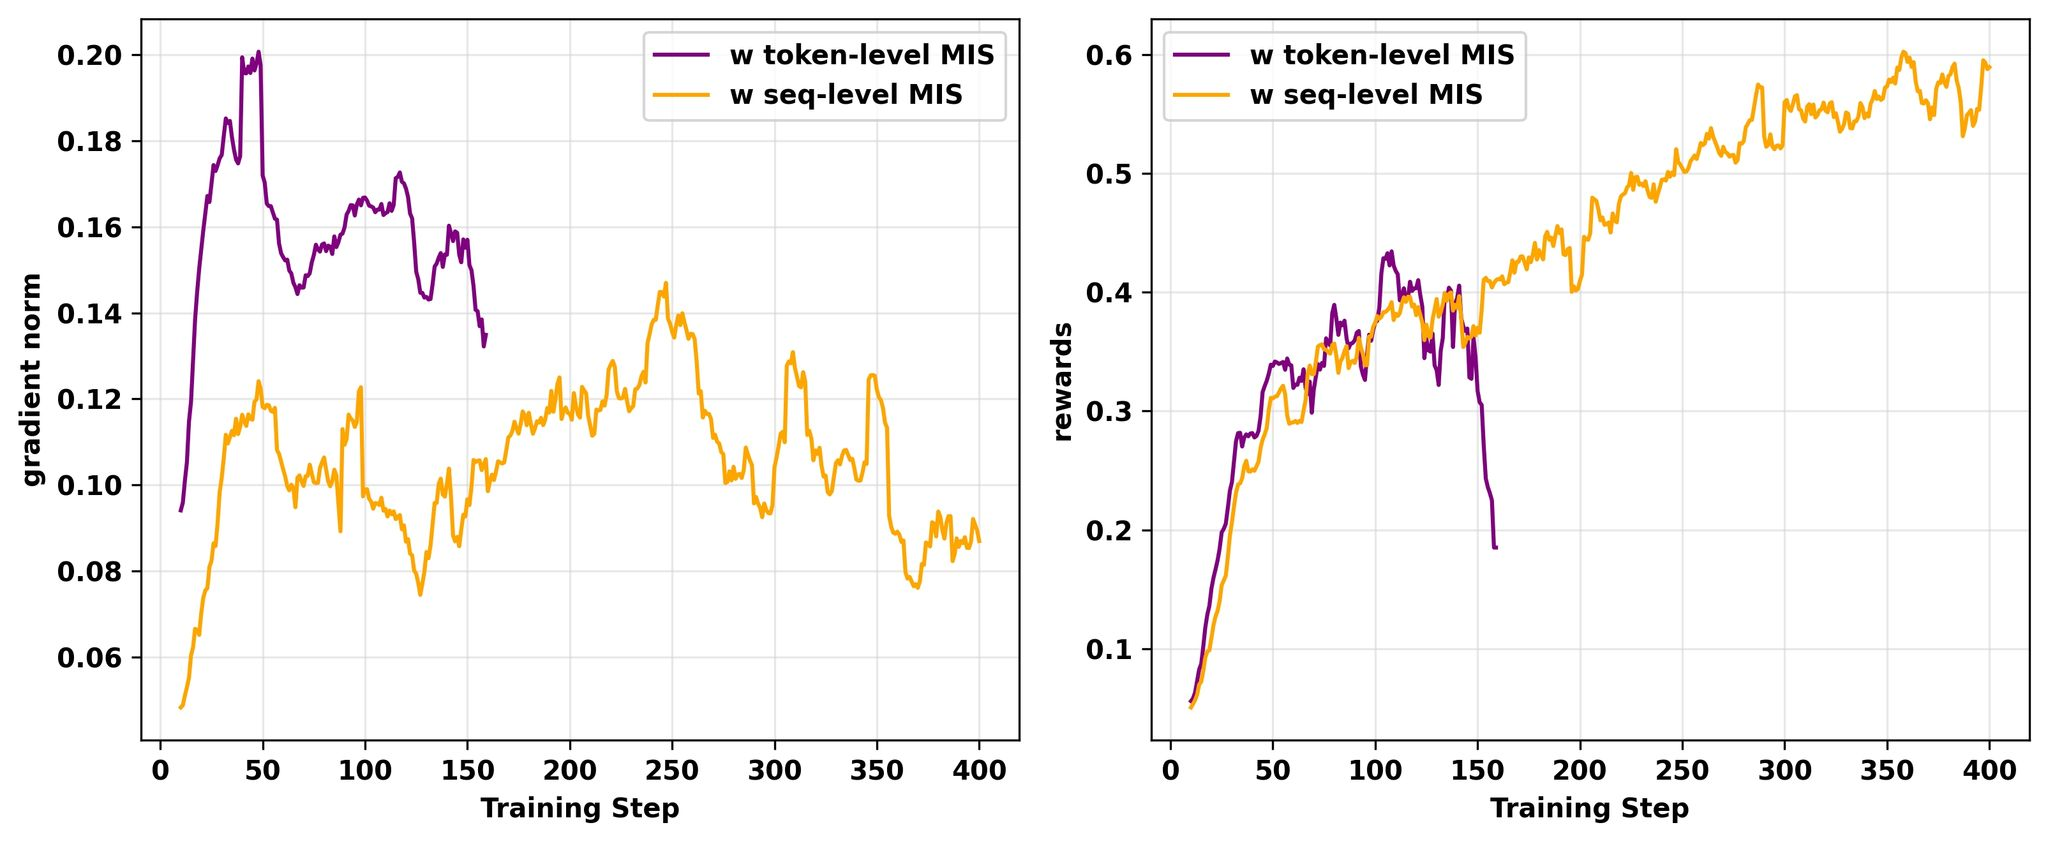
\includegraphics[width=\linewidth,height=0.64\textheight,keepaspectratio]{figures/image-25.jpg}
\caption*{\textbf{图 18。}L20 上同配置的同策略 GRPO：词元级 MIS 与序列级 MIS 的比较。左：梯度范数；右：训练奖励。}
\end{figure}


% source-block: 271211a5-58b7-80f8-a38a-dae34f381bef (sub_sub_header; source-index: 252)

\hypertarget{src-271211a5-58b7-80f8-a38a-dae34f381bef}{}
\subsubsection*{4.2.2 Top-$p$ 采样}


% source-block: 271211a5-58b7-809c-9cf7-ce530f69f705 (text; source-index: 253)

如前所述，vLLM 策略的低概率词元更容易遭受严重的训练与推理不匹配，使 FSDP 策略为其赋予极低概率。为进一步验证这一点，我们开展了 top-$p$ 消融实验。在 L20 GPU 上运行同策略 GRPO，将 vLLM 采样策略的 \code{top-p} 分别设为 0.98、0.99 和 0.999；这里没有使用重要性采样进行梯度修正。

通过减小 \code{top-p}，我们希望降低推理阶段出现极低 vLLM 概率词元的频率，从而缓解训练与推理不匹配。图 19 与预期一致：更小的 \code{top-p} 减少了 \code{vllm-kl} 尖峰。不过，更小的 \code{top-p} 也会增大 vLLM 策略 $\piv$ 与 FSDP 策略 $\pif$ 的分布差异。因此，在没有使用 TIS 时，梯度偏差增大，\code{top-p} 越小，奖励提升越慢。


% source-block: 271211a5-58b7-80a0-9f28-d37a3e81825e (image; source-index: 254)

\begin{figure}[H]
\centering
% source-block: 271211a5-58b7-80a0-9f28-d37a3e81825e (image)
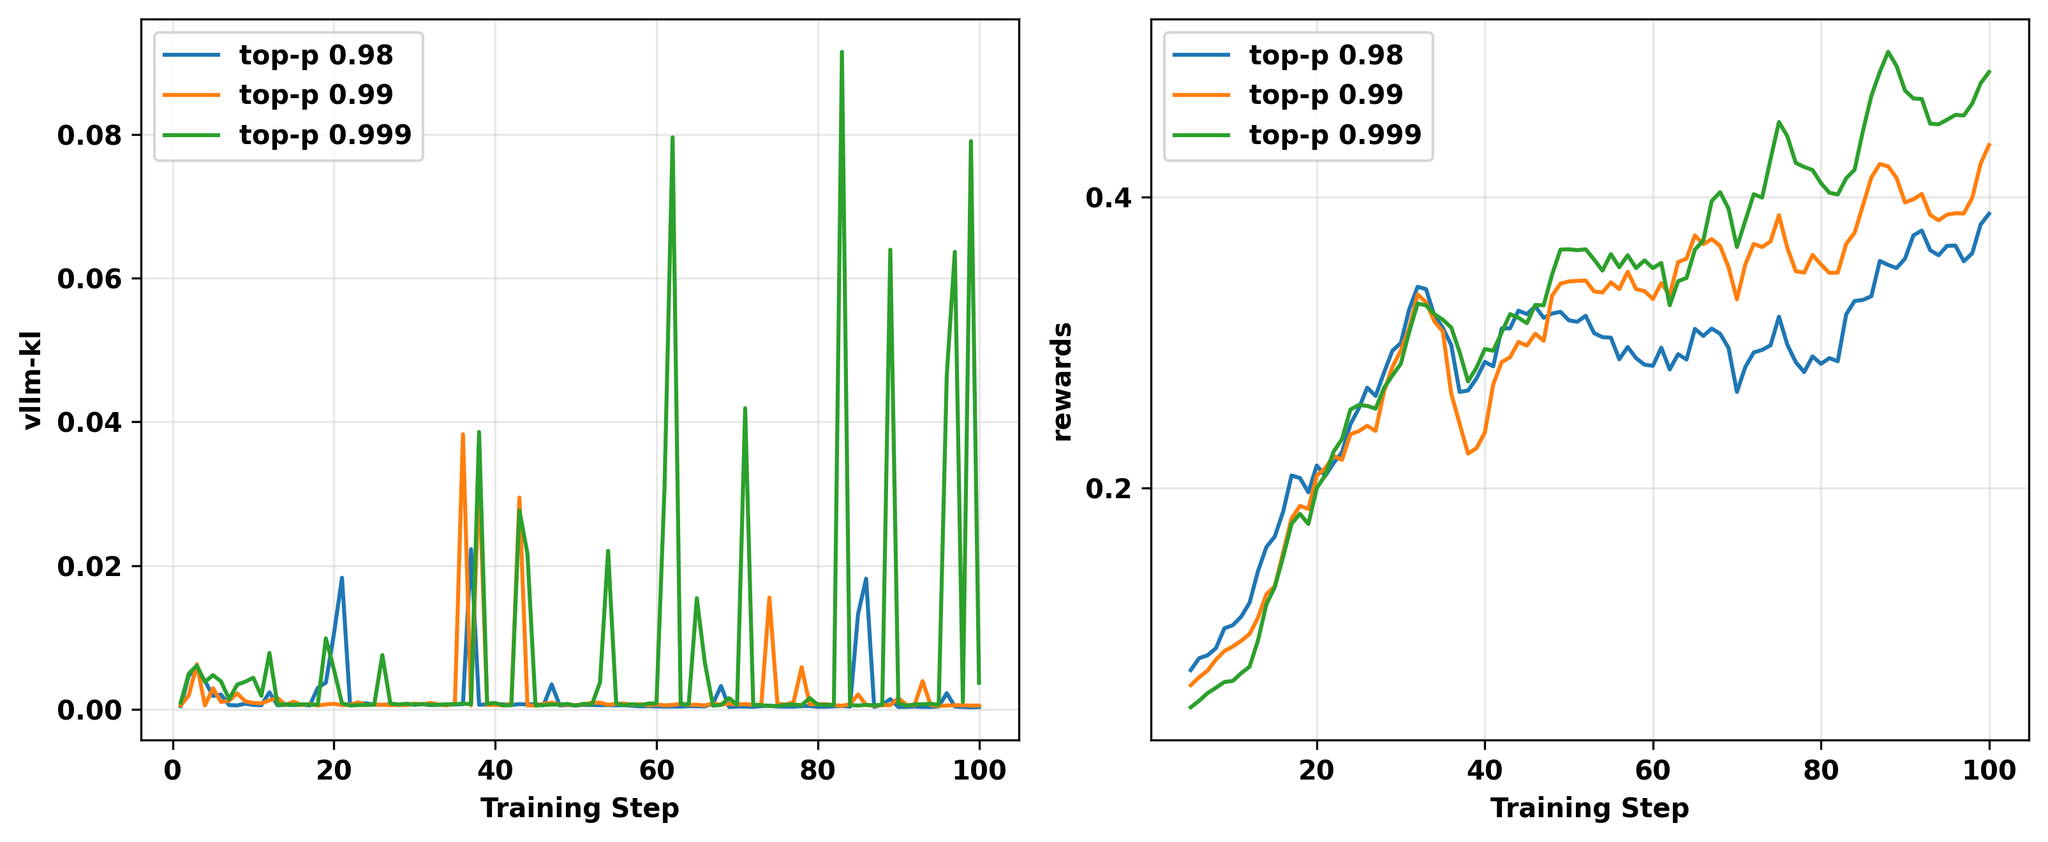
\includegraphics[width=\linewidth,height=0.64\textheight,keepaspectratio]{figures/image-26.png}
\caption*{\textbf{图 19。}强化学习中 vLLM 采样策略的 \code{top-p} 消融。同策略 GRPO 的 \code{top-p} 分别为 0.98、0.99 和 0.999。更小的 \code{top-p} 通常对应更小的 \code{vllm-kl}，但奖励提升也更慢。左：\code{vllm-kl}；右：训练奖励。}
\end{figure}


% source-block: 271211a5-58b7-8013-9729-e1f74e6c65ae (sub_sub_header; source-index: 255)

\hypertarget{src-271211a5-58b7-8013-9729-e1f74e6c65ae}{}
\subsubsection*{4.2.3 使用其他 GPU 系列}


% source-block: 271211a5-58b7-8099-83b6-cfe6b0b5c1e7 (text; source-index: 256)

发现 H20 上的训练与推理不匹配显著小于 L20 后，我们将所有 TIR 实验迁移到 H20，大幅减少了训练崩溃。图 20 展示了在完全相同配置下，分别使用 L20 与 H20 从头训练的两个同策略 GRPO 实验。H20 上的实验显著延长了稳定训练时间，并取得了更好的性能。


% source-block: 271211a5-58b7-8095-9c63-f3bcc7bbef56 (image; source-index: 257)

\begin{figure}[H]
\centering
% source-block: 271211a5-58b7-8095-9c63-f3bcc7bbef56 (image)
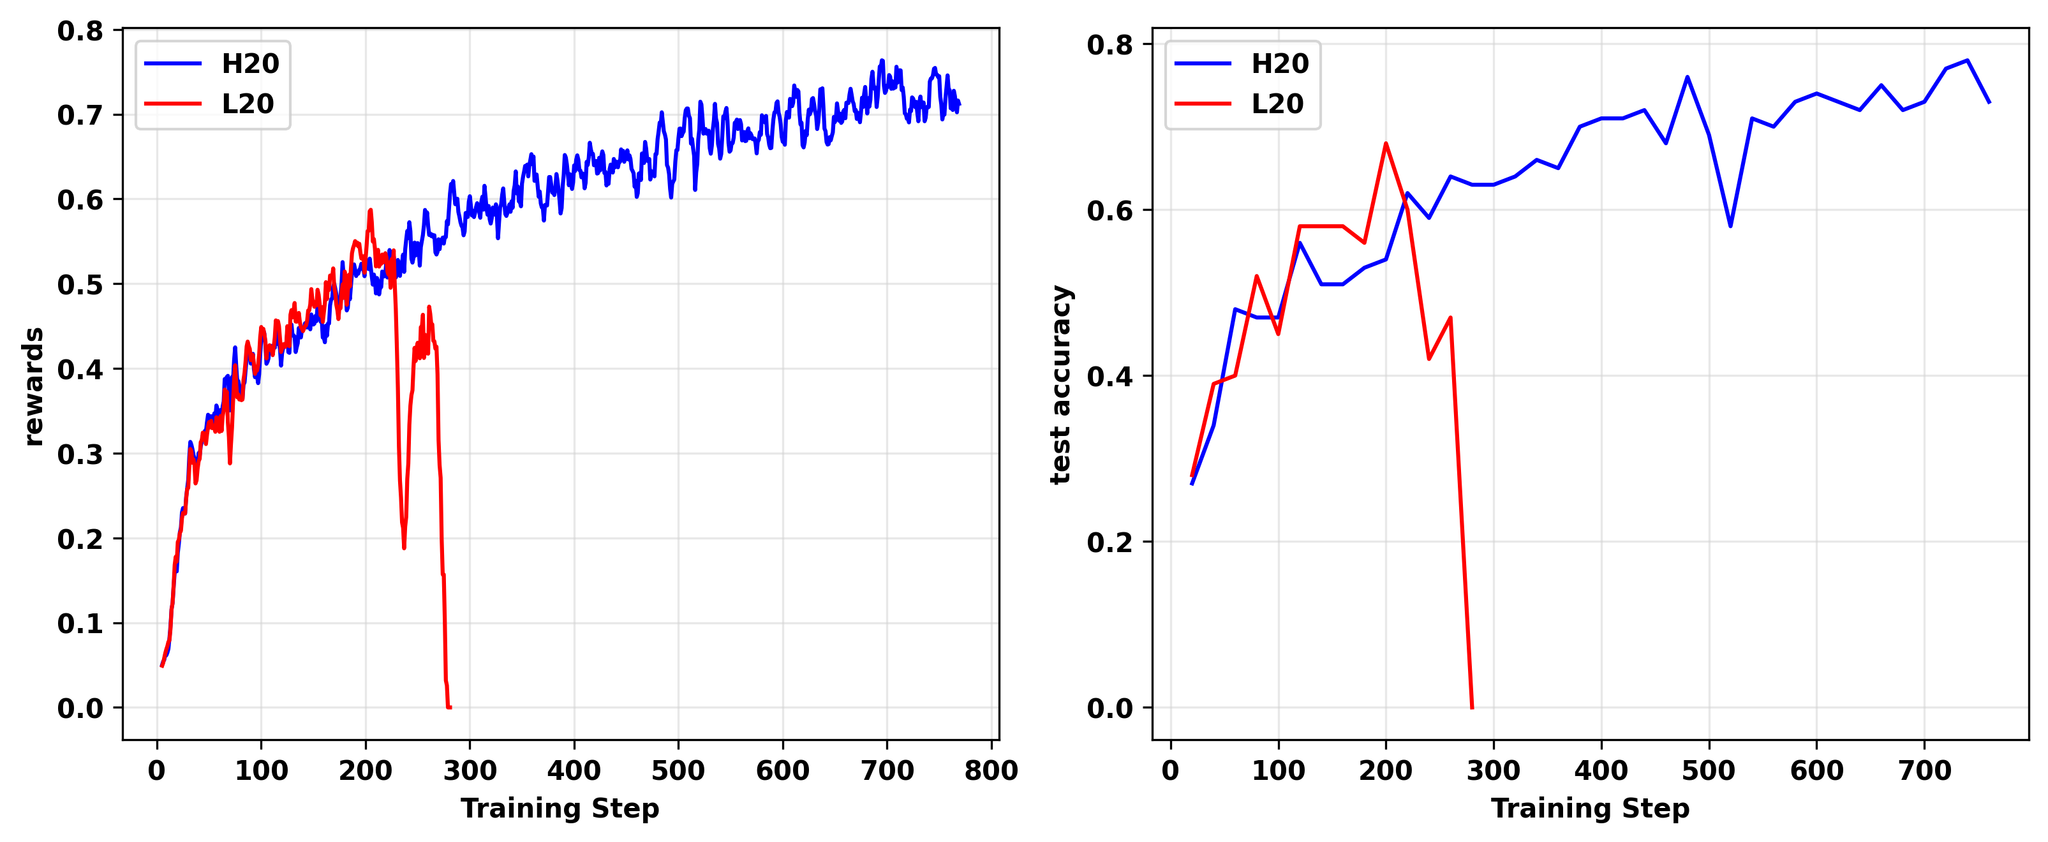
\includegraphics[width=\linewidth,height=0.64\textheight,keepaspectratio]{figures/image-27.png}
\caption*{\textbf{图 20。}分别在 L20 与 H20 上运行的两个同策略 GRPO 实验。左：训练奖励；右：测试准确率。}
\end{figure}


% source-block: 27a211a5-58b7-80fa-b2d9-d85708b21084 (sub_sub_header; source-index: 258)

\hypertarget{src-27a211a5-58b7-80fa-b2d9-d85708b21084}{}
\subsubsection*{4.2.4 关闭 vLLM 的级联注意力}


% source-block: 27a211a5-58b7-8064-b138-d3309bc466a0 (text; source-index: 259)

根据这个 \href{https://github.com/vllm-project/flash-attention/pull/87}{GitHub 讨论}，我们在初始化 vLLM 时设置 \code{disable_cascade_attn=True}，发现它能显著减小 A100 实验中的训练与推理不匹配。我们在 A100 上，以 Qwen3-14B-Base 为基础模型进行两个同策略 GRPO 实验，分别将 \code{disable_cascade_attn} 设为 \code{True} 和 \code{False}。图 21 表明，关闭级联注意力后，\code{vllm-kl} 从 $5\times10^{-2}$ 至 $10^{-1}$ 降至约 $10^{-3}$，不匹配大幅减小；训练集上的奖励也相应提高。


% source-block: 27a211a5-58b7-8082-b200-d1681ccb6ceb (image; source-index: 260)

\begin{figure}[H]
\centering
% source-block: 27a211a5-58b7-8082-b200-d1681ccb6ceb (image)
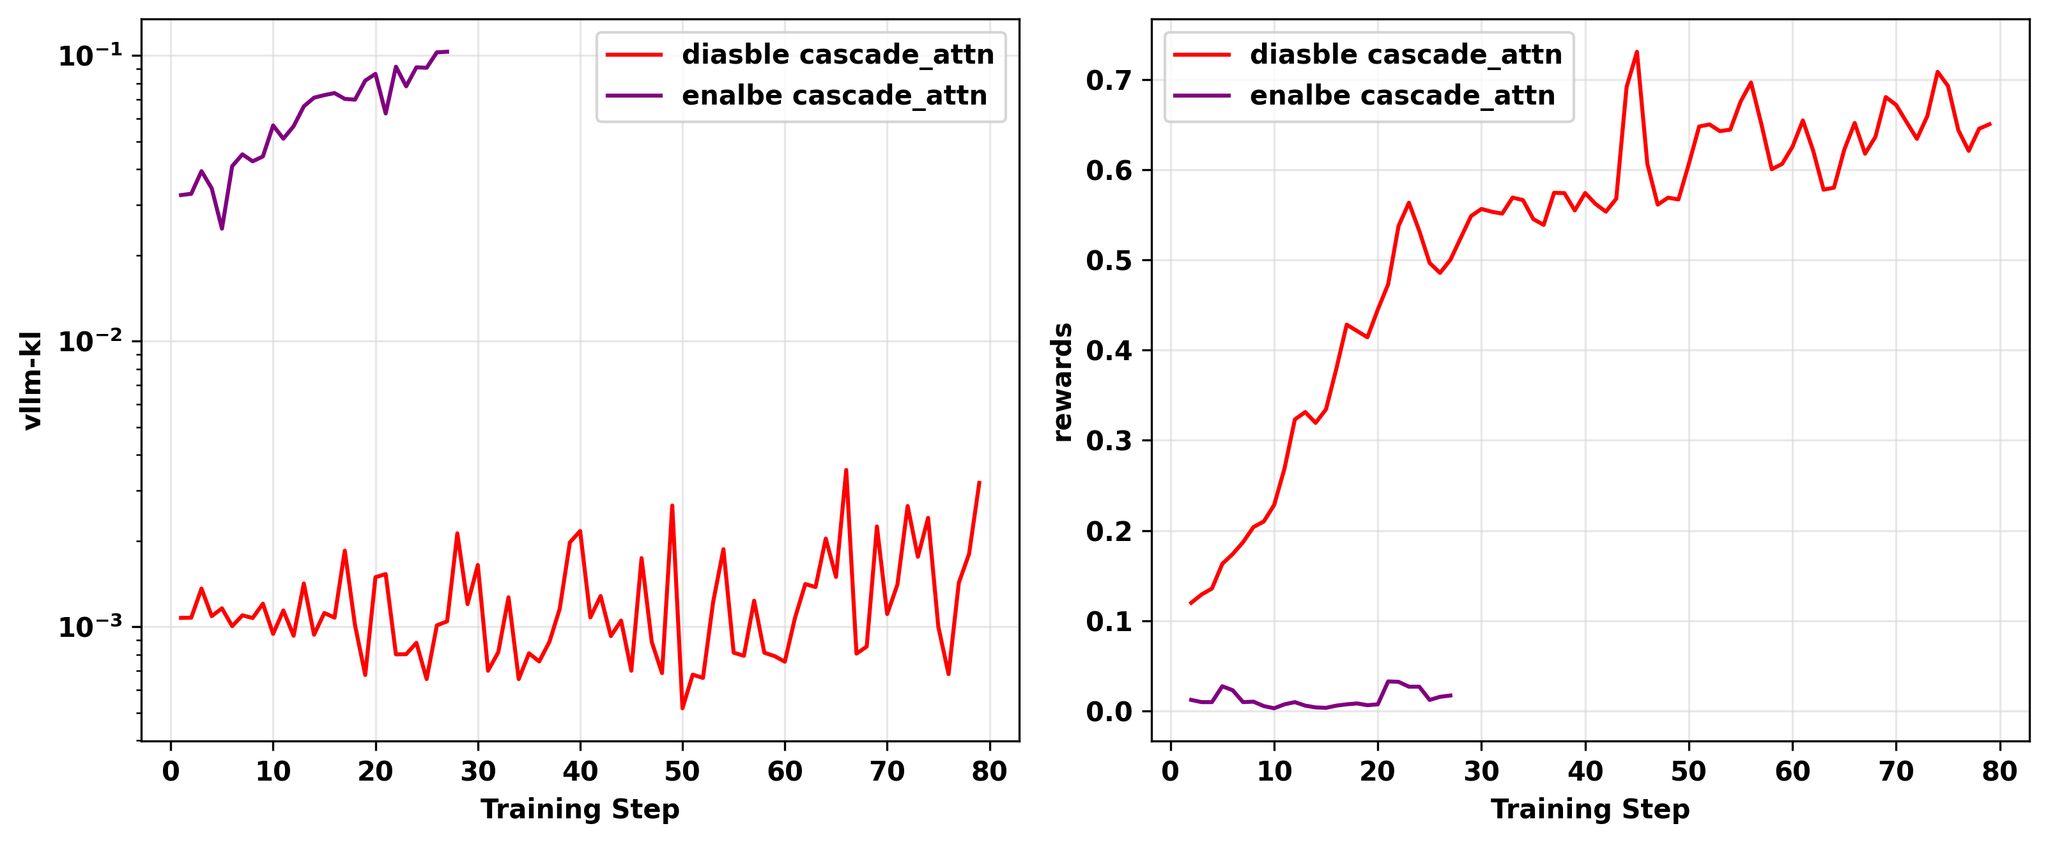
\includegraphics[width=\linewidth,height=0.64\textheight,keepaspectratio]{figures/image-28.png}
\caption*{\textbf{图 21。}级联注意力的消融实验。在 A100 上运行两个同策略实验：一个启用级联注意力，另一个使用相同配置但关闭级联注意力。左：\code{vllm-kl}；右：训练奖励。}
\end{figure}


% source-block: 277211a5-58b7-806a-8461-c2c69bf1c100 (divider; source-index: 261)

% Chinese translation assembled from source/blocks.json.

% See source/translation.py for the translation and source/build_tex.py for assembly.

% source-block: 271211a5-58b7-807d-aec4-ddd7af54a0b0 (header; source-index: 262)

\hypertarget{src-271211a5-58b7-807d-aec4-ddd7af54a0b0}{}
\section*{5. 结论与实践要点}
\phantomsection
\addcontentsline{toc}{section}{5. 结论与实践要点}


% source-block: 277211a5-58b7-8082-b87c-f9ff4d540628 (text; source-index: 263)

训练与推理不匹配是现代推理强化学习与智能体强化学习中一个基础性且不断加剧的挑战，其背后是对性能的持续追求。我们的研究为诊断与缓解这一问题提供了清晰路径。


% source-block: 277211a5-58b7-801f-9a04-c7a042c03742 (bulleted_list; source-index: 264)

\begin{itemize}

\item \textbf{不匹配是一种不可避免的权衡。}应当接受高速推理与训练计算之间总会存在差异；这是一项核心权衡。

% source-block: 277211a5-58b7-80b9-b4fd-f9f021aa562d (bulleted_list; source-index: 265)

\item \textbf{监控训练健康状况。}\code{vllm-kl} 是重要的早期预警指标。应将它与困惑度和梯度范数一起追踪，以便在崩溃之前预测、诊断不稳定性。

% source-block: 277211a5-58b7-804c-8ba9-f871c1bc24de (bulleted_list; source-index: 266)

\item \textbf{识别真正的触发因素。}问题并非随机发生，而是由低概率词元系统性触发。当模型处理分布外输入时，这些词元出现得更频繁；工具使用和多轮应用中，这种场景十分常见。

% source-block: 277211a5-58b7-805e-b7ee-f6c68cdddf4b (bulleted_list; source-index: 267)

\item \textbf{硬件是关键变量。}同样的代码可能在一种 GPU 架构上崩溃，却在另一种架构上正常训练。应始终在目标硬件上验证配置，因为实验结果未必能完全迁移。

% source-block: 277211a5-58b7-8092-8fb5-d43746fdd375 (bulleted_list; source-index: 268)

\item \textbf{采用有理论依据的修正。}更换硬件或调整采样器可以提供帮助，而最稳健、有原理支撑的方案仍在算法层面。我们的工作表明，有理论偏差的词元级修正并不充分，在实验中仍可能失败。相比之下，序列级截断重要性采样（Seq-TIS）和掩码重要性采样（Seq-MIS）通过修正完整状态轨迹，直接处理梯度偏差。作者认为，这些方法对于维持稳定性至关重要，应作为严肃 LLM-RL 训练栈的默认考虑。

\end{itemize}

% source-block: 277211a5-58b7-8013-b186-f5d0c4c4b315 (text; source-index: 269)

我们推测，推理引擎（如 vLLM）与训练框架（如 Megatron-LM）之间的不匹配，也将成为混合专家模型（MoE）强化学习的重要问题。这是未来值得研究的关键方向。


% source-block: 278211a5-58b7-807a-b606-fa0c8a6818f8 (text; source-index: 270)

\end{document}
